% This is a LaTeX thesis template for Adam Mickiewicz University.
% to be used with quarto
% This template was produced by Jakub Nowosad
% Version: 22 July 2023

% Inspired by:
% This is a LaTeX thesis template for Monash University.
% to be used with Rmarkdown
% This template was produced by Rob Hyndman
% Version: 6 September 2016

\documentclass{amuthesis}
\usepackage{polski}
%\usepackage[polish]{babel}
%\addto\captionspolish{\renewcommand{\figurename}{Rycina}}
%\addto\captionspolish{\renewcommand{\tablename}{Tabela}}
\renewcommand{\figurename}{Rycina} % Redefine default figure caption %
\renewcommand{\tablename}{Tabela} % Redefine default table caption %
%%%%%%%%%%%%%%%%%%%%%%%%%%%%%%%%%%%%%%%%%%%%%%%%%%%%%%%%%%%%%%%
% Add any LaTeX packages and other preamble here if required
%%%%%%%%%%%%%%%%%%%%%%%%%%%%%%%%%%%%%%%%%%%%%%%%%%%%%%%%%%%%%%%
\usepackage{booktabs,tabularx} % Allows kableExtra to work %
\usepackage{indentfirst} % Adds indent in the first paragraph %
\usepackage{bookmark} % Adds indent in the first paragraph %

\author{Mateusz Rydzik}
\title{Ocena wpływu tworzenia nowych lądów na jakość wód przy
wykorzystaniu danych teledetekcyjnych}
\def\titleeng{Assessment of the impact of land reclamation on water
quality using remote sensing data}
\def\degreetitle{Praca magisterska}
\def\major{Geoinformacja}
\def\albumid{455820}
\def\thesisyear{2024}

% Add subject and keywords below
\hypersetup{
     %pdfsubject={The Subject},
     %pdfkeywords={Some Keywords},
     pdfauthor={Mateusz Rydzik},
     pdftitle={Ocena wpływu tworzenia nowych lądów na jakość wód przy
wykorzystaniu danych teledetekcyjnych},
     pdfproducer={quarto with LaTeX}
}

\bibliography{thesis.bib, packages.bib}

\begin{document}

\pagenumbering{arabic}

\titlepage

\bookmarksetup{startatroot}

\hypertarget{streszczenie}{%
\chapter*{Streszczenie}\label{streszczenie}}
\addcontentsline{toc}{chapter}{Streszczenie}

\markboth{Streszczenie}{Streszczenie}

\textbf{Abstrakt}

Tworzenie nowych lądów polega na sztucznym przekształcaniu obszarów
wodnych w tereny lądowe. Procesy te wpływają na ekosystemy wodne,
stanowiąc potencjalne zagrożenie dla występujących w nich organizmów.
Wzrost liczby ludności, zamieszkującej wybrzeża może doprowadzić do
nasilenia się procesów tworzenia nowych lądów. Celem pracy jest ocena
potencjalnego wpływu procesów tworzenia nowych obszarów lądowych na
jakość pobliskich wód. Do oceny jakości wód wykorzystane zostały
wskaźniki spektralne, obliczone przy wykorzystaniu zdjęć satelitarnych.
Wskaźniki te opisują zmiany dwóch parametrów jakości wód: stężęń
chlorofilu a i zawiesiny. Badania przeprowadzono dla pięciu obszarów, na
których powstały nowe lądy: Dubaj (Zjednoczone Emiraty Arabskie), Lagos
(Nigeria), Limon (Kostaryka), Singapur i Szanghaj (Chiny). Wskaźniki
spektralne wykryły znaczące zmiany jakości wód na obszarach badań w
trakcie tworzenia nowych lądów. Konstrukcja nowych lądów doprowadziła do
spadku stężenia chlorofilu a w Dubaju, Limon i Singapurze. Wzrost
stężęnia chlorofilu a odnotowano w Lagos i Szanghaju. Podczas trwania
budowy nowych obszarów lądowych, w Dubaju, Limon i Szanghaju
zaobserwowano wzrost stężenia zawiesiny w wodzie. W Lagos i Singapurze
wykryto długookresowy spadek stężenia zawiesiny.

Słowa kluczowe: (wskaźniki spektralne, obrazy satelitarne, jakość wód,
tworzenie lądów)

\textbf{Abstract}

Land reclamation involves the artificial transformation of water areas
into land areas. These processes affect water ecosystems, posing
potential threats to the organisms living within them. The increase in
coastal population may lead to an intensification of land reclamation
processes. The aim of this study is to assess the potential impact of
land reclamation processes on the quality of nearby waters. Spectral
indices, calculated using satellite images, were used to assess water
quality. These indices describe changes in two water quality parameters:
chlorophyll-a concentration and suspended matter concentration. The
study was conducted in five areas where new lands have been created:
Dubai (United Arab Emirates), Lagos (Nigeria), Limon (Costa Rica),
Singapore, and Shanghai (China). Spectral indices detected significant
changes in water quality in the study areas during the land reclamation.
The construction of new lands led to a decrease in chlorophyll-a
concentration in Dubai, Limon, and Singapore. An increase in
chlorophyll-a concentration was observed in Lagos and Shanghai. During
the construction of new land areas, an increase in suspended matter
concentration in the water was observed in Dubai, Limon, and Shanghai.
In Lagos and Singapore, a long-term decrease in suspended matter
concentration was detected.

Keywords: (spectral indices, satellite images, water quality, land
reclamation)

\newpage

\setstretch{1.2}\sf\tighttoc\doublespacing

\bookmarksetup{startatroot}

\hypertarget{sec-wprowadzenie}{%
\chapter{Wprowadzenie}\label{sec-wprowadzenie}}

Wzrost liczby ludności jest zjawiskiem, które znacząco wpływa na wiele
aspektów społeczno-gospodarczych. Wymusza ono utworzenie nowych obszarów
mieszkalnych, zwiększenia produkcji żywności oraz pozostałych dóbr,
usprawnienie infrastruktury transportowej i wszystkich innych elementów
pośrednich. Każda z tych czynności oddziaływuje w różnych stopniach na
środowisko przyrodnicze \autocite{cropper1994interaction}.

Jednym z elementów środowiska szczególnie narażonym na negatywne
zjawiska związane ze wzrostem populacji jest środowisko wodne. Ponad
połowa ludności na świecie zamieszkuje obszary przybrzeżne
\autocite{seto2011meta}. Jednocześnie wykazywany jest trend migracji
ludności do miast znajdujących się na wybrzeżu
\autocite{hugo2011future}, który może przyczynić się do zwiększenia
udziału populacji zamieszkującej miasta nadmorskie w ogólnej sumie
populacji na świecie \autocite{mcgranahan2007rising}. Oznacza to, że
wszystkie czynności służące przygotowaniu miast do przyjęcia nowych
mieszkańców będą wpływały również na morza i oceany.

Do metod dostosowywania miast do nowych mieszkańców można zaliczyć
przekształcanie istniejących form wykorzystania terenu na obszary
mieszkalne lub usługowe. Może to w pewnym momencie spowodować brak
dostępnych obszarów lądowych do osiedlenia w nadmorskich miastach. Jedną
z alternatyw pozyskiwania nowych lądów może być proces tworzenia nowych
lądów.

Jednym z krajów, zaliczanych do pionierów pozyskiwania nowych lądów,
jest Holandia, na obszarze której już w 1533 roku przekształcono jezioro
w nowe tereny do zagospodarowania \autocite{ven1993man}. Operacja ta nie
została jednak podyktowana zapotrzebowaniem na nowe tereny, a wymuszona
przez ciągłe rozrastanie się jeziora i zalewanie pobliskich
miejscowości. Proces tworzenia nowego lądu polegał na wypompowaniu wody
z jeziora do wybudowanej wokół niego sieci kanałów, i odprowadzenia jej
do jeziora Zuiderzee. Dna zbiorników, nazywanych polderami,
wykorzystywane były przede wszystkim do rolnictwa. W celu konserwacji
nowo pozyskanych terenów, ziemie podzielone zostały sieciami kanałów,
ułatwiających odprowadzanie wody poza poldery. Rowy te jednocześnie
wykorzystano jako granice działek, dzieląc nowy ląd na siatkę parceli o
charakterystycznych, regularnych kształtach
\autocite{hoeksema2007three}. Wraz z upływem lat, procesy tworzenia
nowych lądów w Holandii były stale rozwijane. Punktem kulminacyjnym była
seria konstrukcji nowych prowincji w XX wieku, których rezultatem było
pozyskanie dla Holandii lądów o łącznej powierzchni 1650 kilometrów
kwadratowych. Stanowił to wzrost powierzchni kraju o 5\%
\autocite{hoeksema2007three}.

Współcześnie, stosowane są inne metody konstrukcji terenów lądowych.
Oprócz polderów, stosowane są techniki usypywania materiału na dnie
zbiornika do momentu wydobycia się go ponad powierzchnię wody.
Najczęściej stosowanym materiałem jest piasek, często mieszany z
większymi skałami czy cementem \autocite{martin2016review}. Piasek może
być usypywany przy wybrzeżu, poszerzając go wgłąb morza. Innym
rozwiązaniem jest usypywanie materiału z dala od lądu, tworząc sztuczne
wyspy. Oprócz tworzenia nowych stref mieszkalnych, nowe lądy tworzone są
do: rozbudowy portów i lotnisk, pozyskiwania terenów rolniczych czy
tworzenia nowych stref wojskowych \autocite{martin2016review}. Procesy
te są szczególnie widoczne w megamiastach, czyli ogromnych miastach o
populacji przekraczającej osiem milionów mieszkańców
\autocite{wenzel2007megacities}. W 16 wybranych megamiastach przez
ostatnie 40 lat utworzono 1249 kilometrów kwadratowych nowych lądów
\autocite{sengupta2018building}. Aż 587 kilometrów kwadratowych nowych
ziem z tej sumy utworzono w Szanghaju, które w tym okresie powiększyło
swoją powierzchnię o 6,5\% \autocite{sengupta2018building}. Biorąc pod
uwagę prognozy wzrostu liczby ludności zamieszkującej wybrzeża, możliwe
jest przypuszczenie o zwiększeniu natężenia tworzenia nowych lądów.
Procesy te mogą okazać się jedyną możliwą decyzją dla obszarów, które
mają ograniczoną ilość dostępnych obszarów. Ograniczenie obszarów można
rozumieć jako fizyczny brak terenów, albo jako restrykcje, nałożone w
ramach programów ochrony środowiska. Powoduje to powstawanie wielu pytań
odnośnie bezpieczeństwa tych procesów w kontekście ochrony środowiska.
Współczesne metody tworzenia nowych lądów wymagają pozyskania dużej
ilości piasku, najczęściej z dna zbiorników wodnych lub istniejących
wysp. Konieczne jest ustalenie relacji między procesami tworzenia nowych
lądów a ich wpływem na środowisko. W tej pracy, nacisk został położony
na jeden z aspektów jakości wody.

Jakość wód badana jest przeważnie na podstawie trzech grup parametrów:
fizycznych, chemicznych i biologicznych \autocite{summers2020water}. Do
fizycznych parametrów przynależą takie własności jak temperatura, kolor,
smak wody, czy występowanie zawiesiny \autocite{summers2020water}.
Chemiczne parametry badają występowanie metali ciężkich, substancji
toksycznych lub sam odczyn wody \autocite{summers2020water}. Do
biologicznych parametrów zalicza się występowanie bakterii, alg, oraz
wirusów \autocite{summers2020water}. Podstawowym sposobem badania
jakości wód jest wykonywanie pomiarów w terenie. Jest to jednak proces
kosztowny oraz czasochłonny, wymagający ręcznego pobierania próbek na
obszarze badań i ich transportu do laboratorium
\autocite{glasgow2004real}. Manualne pomiary coraz częściej są
zastępowane przez mierniki, które automatycznie albo poprzez zdalne
wywołanie dokonują pomiarów. Taka automatyzacja umożliwia
przeprowadzanie ciągłego monitoringu stanu wód, bez konieczności
fizycznego przebywania nad zbiornikiem \autocite{glasgow2004real}.
Dodatkowym źródłem cennych informacji o stanie jakości wód są zdjęcia
satelitarne. Pozwalają one na ocenę wybranych parametrów, w
szczególności fizycznych. Dużą zaletą zdjęć satelitarnych jest także ich
rozdzielczość przestrzenna. Zdjęcie jest w stanie dostarczyć informacji
dla większego obszaru badań niż pojedyncze pomiary punktowe.

Mając na uwadze potencjalny wzrost zapotrzebowania na tereny w miastach
nadmorskich, konieczne jest zbadanie wpływu konstrukcji nowych ziem na
środowisko. Celem pracy było zbadanie potencjalnego wpływu tworzenia
nowych lądów na zmiany jakości pobliskich wód. Wybranych zostało pięć
obszarów badań, na terenie których dokonano konstrukcji nowych lądów w
przeciągu ostatnich 30 lat. Stan wód był badany w trzech etapach: przed,
w trakcie i po zakończeniu prac konstrukcyjnych. Jakości wód zostały
porównane między obszarami badań, w celu wykrycia potencjalnych
przestrzennych lub czasowych trendów. Do wykonania oceny jakości wód
korzystano dane teledetekcyjne w postaci zdjęć satelitarnych, przy
pomocy których obliczono wskaźniki spektralne.

\bookmarksetup{startatroot}

\hypertarget{sec-lit}{%
\chapter{Przegląd literatury}\label{sec-lit}}

Badania odnośnie wpływu konstrukcji lądów na jakość wód są istotne przez
stale rosnącą liczbę ludności, w szczególności w obszarach na wybrzeżach
\autocite{mcgranahan2007rising}. Nowe lądy znajdują zastosowania w
poszerzaniu granic przybrzeżnych miast, dostarczając tereny pod strefy
mieszkalne i przemysłowe \autocite{wang2014development}. Ocena wpływu
konstrukcji nowych lądów na stan jakości wód jest tematem wielu badań,
których wyniki wykorzystano w tej pracy. Jakość wody rozumiana jest jako
opis charakterystyki wody, określających jej przydatność do
wykorzystywania w wielu dziedzinach. Jakość wody jest oceniana na
podstawie fizycznych, chemicznych i biologicznych parametrów
\autocite{tyagi2013water}.

Zaletą danych teledetekcyjnych w ocenie jakości wód jest zasięg, którym
obejmują ciągły obszar badań \autocite{gholizadeh2016comprehensive}.
Pozwala to na obserwacje przestrzennego rozkładu stanu wód, w
przeciwieństwie do punktowych pomiarów w terenie, które dostarczają
informacje jedynie o stanie konkretnego punktu w przestrzeni.
Wykorzystanie zdjęć satelitarnych jako danych teledetekcyjnych ogranicza
jednak liczbę właściwości wody, jaką można ocenić. Pozwalają one głównie
na badanie fizycznych właściwości wód, takich jak ich kolor czy mętność
\autocite{glasgow2004real}. Stacje pomiarowe w terenie pozwalają na
pozyskanie większej ilości informacji, opisujących chemiczne i
biologiczne własności wody \autocite{summers2020water}. Znaczna liczba
badań zbiorników wodnych przy wykorzystaniu danych teledetekcyjnych
skupia się na ocenie występowania chlorofilu a oraz stężenia
zawieszonego materiału \autocite{gholizadeh2016comprehensive}.

Zespół \textcite{zhang2017assessment} prowadził badania na obszarze
zatoki Jiaozhou w Chinach. Wybrzeże tej zatoki ulegało przekształceniom,
będących wynikiem wielu prac konstrukcji nowych lądów. Część z nowych
terenów wykorzystano do rozwoju przemysłu. Wraz ze wzrostem natężenia
konstrukcji nowych lądów, odnotowano wzrost stężenia nieorganicznego
azotu, rozpuszczonego w wodach zatoki Jiaozhou. W ramach tej pracy,
zdecydowano się zbadać wpływ wybranych czynników na zmiany stężenia
nieorganicznego azotu w zatoce Jiaozhou, które mogła doprowadzić do
zmian jakości wody. Do oceny jakości wód, zespół pozyskał zbiory danych
pochodzące z pomiarów w terenie. Dane te opisują właściwości wody,
których zmiany w stężeniu występowania w wodzie mogą świadczyć o
potencjalnym pogorszeniu lub polepszeniu jakości wód. Do zbioru danych,
oprócz stężenia azotu odprowadzanego przez rzeki do zbiornika, zaliczono
również informacje o: stężeniu chlorofilu a, zasadowości i temperaturze
wody, zasoleniu czy ilości rozpuszczonego tlenu. Dane następnie
podzielono na dwie grupy: czynniki wpływu antropogenicznego
(przedostawanie się azotu i innych związków do zbiorników wodnych
bezpośrednio przez strefy przemysłowe, lub odprowadzone do rzek
uchodzących w zatoce) oraz przyrodnicze czynniki strefy przybrzeżnej
(stężenie chlorofilu a i zawiesiny w wodzie, temperatura i zasolenie
wody, oraz zjawiska przyrodnicze). W pracy wykorzystano metody
statystyczne, między innymi regresję liniową, analizę czynnikową oraz
numeryczne modele jakości wód, do zbadania wpływu poszczególnych
elementów zbioru danych na zmiany stężenia rozpuszczonego azotu w
zatoce. Praca wskazała, że głównymi czynnikami pogorszenia jakości wód w
zatoce Jiaozhou był wzrost stężenia nieorganicznego azotu odprowadzanego
przez rzeki do zatoki, oraz jednoczesne zmniejszanie powierzchni
zbiornika wodnego. Tworzenie nowych lądów w zatoce skutkowało
przekształcaniem powierzchni zatoki Jiaozhou między innymi w obszary
przemysłowe, które zwiększały stężenie nieorganicznego azotu w wodach
zatoki. Autorzy wskazali na konieczność wprowadzenia programów
uzdatniania wody z rzek, czy przenoszenia stref przemysłowych z dala od
wybrzeża w celu poprawienia jakości wód w zbiorniku.

Praca \textcite{hao2021effects} skupia się na określeniu wpływu
konstrukcji nowych terenów w mieście Ningbo na stan jakości wód w zatoce
Hangzhou w Chinach. Do oceny jakości wód wybrano cztery metale ciężkie:
miedź, ołów, cynk i kadm. Wzrost stężenia tych metali w wodzie został
utożsamiony z pogorszeniem jakości wody. Dane pozyskano z próbek,
pobranych w trzech okresach: przed rozpoczęciem prac (2007 rok), tuż po
zakończeniu prac (2016 rok) i dłuższy czas po zakończeniu prac (2018
rok). Próbkowanie stężenia metali ciężkich w trzech oddzielnych etapach
pozwoliło na ocenę wpływu tworzenia nowych lądów na stan jakości wód,
porównując ilość metali ciężkich po zakończeniu prac z ilością przed
rozpoczęciem prac. Badania wskazały na najwyższe wartości trzech z
czterech metali ciężkich w 2016 roku, czyli tuż po zakończeniu prac.
Jedynym metalem ciężkim, którego ilość była większa przed rozpoczęciem
prac niż tuż po zakończeniu prac był kadm. Największy wzrost tuż po
zakończeniu prac, w porównaniu do stanu przed rozpoczęciem prac,
odnotowały miedź oraz cynk. Obserwując stężenia metali ciężkich w 2018
roku, czyli dwa lata po zakończeniu prac, zauważyć można spadek ich
stężenia do stanu przed rozpoczęciem prac. W przypadku ołowiu, stężenie
metali wykryte w zbiorniku było mniejsze w 2018 roku niż w 2007 roku.
Trend spadku stężenia metali po zakończeniu prac nie został odnotowany
dla kadmu, którego stężenie w wodzie wzrosło dwa lata po zakończeniu
prac. Wyniki badań wskazują na wpływ tworzenia nowych lądów na stan
jakości wody. Tuż po zakończeniu prac, stężenie metali ciężkich w wodach
było większa niż przed rozpoczęciem prac. Wraz z upływem czasu po
zakończeniu prac, stężenie metali w wodzie stopniowo malało.

Praca \textcite{wang2023observations} skupiona jest na badaniu wpływu
budowy lotniska w Hongkongu na jakość pobliskich wód. Jako, że Hongkong
dysponuje ograniczoną ilością terenu, lotnisko zdecydowano się zbudować
na nowo utworzonym lądzie. Do oceny jakości wód autorzy wykorzystali
zdjęcia satelitarne Landsat oraz dane, pochodzące z monitoringu
terenowego. Jakość wód została oceniona głównie przy pomocy parametrów
stężenia zawiesiny i nieorganicznego azotu w wodzie. Po wstępnym
przetworzeniu zdjęć satelitarnych, wartości poszczególnych kanałów
zestawiono z danymi terenowymi. Pozwoliło to na wybór kanałów
widzialnych i bliskiej podczerwieni, na podstawie których obliczono
algorytm estymacji parametrów jakości wody. Algorytmy wykorzystano do
stworzenia modeli, pozwalających na oszacowanie stężenia zawiesiny i
nieorganicznego azotu na podstawie obrazów satelitarnych. Modele te były
trenowane na podstawie danych terenowych. Badania wykazały wzrost
stężenia zawiesiny i nieorganicznego azotu w pobliżu nowego lądu, na
którym znajdowało się lotnisko. Autorzy potwierdzili wpływ tworzenia
nowego lądu, a w szczególności jego wykorzystywania, na stan jakości
wód.

\bookmarksetup{startatroot}

\hypertarget{sec-metody}{%
\chapter{Metody}\label{sec-metody}}

Rozdział ten podzielony jest na podrozdziały, odpowiadające każdemu z
trzech głównych etapów prac: wybór obszarów badań, pozyskiwanie danych
teledetekcyjnych w postaci zdjęć satelitarnych, oraz obliczanie
wskaźników spektralnych i interpretacja wyników.
Rycina~\ref{fig-flowchart} przedstawia schemat prac i wykonywanych
kroków. Wszystkie etapy pozyskiwania danych, ich przetwarzania oraz
prezentowania wyników zostały przeprowadzone przy wykorzystaniu języka
programowania \textbf{R} \autocite{R-base}. Podrozdziały zawierają
odniesienia do wykorzystywanych pakietów R, ułatwiających i
automatyzujących poszczególne etapy prac.

\begin{figure}[t]

{\centering 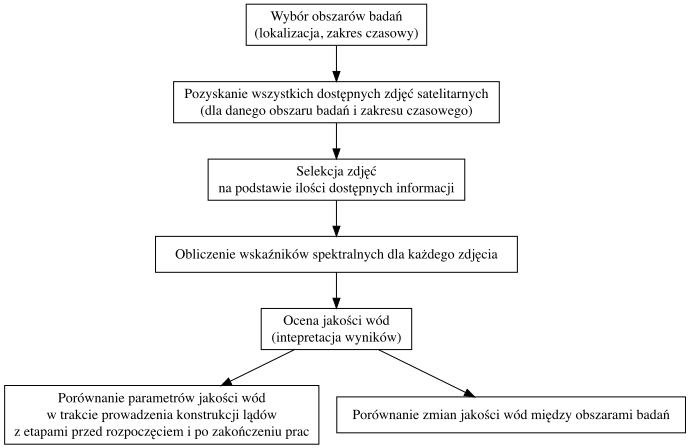
\includegraphics[width=5.20833in,height=\textheight]{figures/flowchart.png}

}

\caption{\label{fig-flowchart}Schemat działań, wykonywanych w ramach
pracy.}

\end{figure}

\hypertarget{wybuxf3r-obszaruxf3w-badaux144}{%
\section{Wybór obszarów badań}\label{wybuxf3r-obszaruxf3w-badaux144}}

Obszary badań obejmowały przybrzeżne tereny lądowe oraz przylegające
zbiorniki wodne, Jako obszar badań rozumiane są granice przestrzenne,
wyznaczone przez cztery pary współrzędnych. Zostały one wybrane na
podstawie przeglądu literatury i artykułów oraz wcześniejszej wiedzy
autora.

Obszar badań musiał spełniać postawione wymagania, żeby został wybrany.
Najważniejszym warunkiem był rok rozpoczęcia prac. Jako, iż praca bazuje
na zdjęciach satelitarnych ze zbiorów Microsoft Planetary Computer,
obszar badań musiał obejmować nowy ląd, którego konstrukcję rozpoczęto
po 1982 roku \autocite{microsoft_open_source_2022_7261897}. Dodatkowo, w
celu porównania stanu jakości wód w trakcie trwania prac ze stanem przed
rozpoczęciem prac i po zakończeniu, konieczne jest uwzględnienie w
badaniach również przedziału czasowego przed i po okresie prowadzenia
prac. W ramach pracy przedział ten ustalono na minimum dwa lata przed i
po zakończeniu prac. Oznacza to, że wybrany obszar badań musiał
obejmować konstrukcję nowego lądu, która rozpoczęła się najwcześniej w
1984 roku. Taki sam warunek postawiono dla roku zakończenia prac. Prace
na wybranym obszarze badań mogły zakończyć się najpóźniej w 2020 roku,
co pozwoliłoby uwzględnić dodatkowe dwa -- trzy lata do porównania
wartości po zakończeniu prac. Dodatkowym warunkiem była powierzchnia
nowo utworzonego lądu. Przy wyborze obszarów badań do pracy skupiono się
na projektach, których zmiany w przebiegu konstrukcji byłyby widoczne z
poziomu obrazów satelitarnych. Wyklucza to mniejsze projekty, których
zmiany nie byłyby zauważalne na zdjęciach satelitarnych Landsat o
rozdzielczości przestrzennej 30 metrów.

Z prac naukowych pozyskano informacje o lokalizacji obszaru, lat
prowadzenia prac oraz wykorzystaniu nowego lądu. Część publikacji
opisujących konstrukcje nowych lądów do okresu prowadzenia prac
zaliczyła również etapy przygotowawcze (badania w terenie, pozyskiwanie
zgód itd.) oraz działania po zakończeniu prac (tworzenie infrastruktury
na nowym lądzie, konstrukcja budowli). W takim przypadku, wykorzystano
serie czasowe obrazów satelitarnych w celu określenia konkretnego roku
rozpoczęcia i zakończenia prac.

\hypertarget{pozyskiwanie-zdjux119ux107-satelitarnych}{%
\section{Pozyskiwanie zdjęć
satelitarnych}\label{pozyskiwanie-zdjux119ux107-satelitarnych}}

Zdjęcia satelitarne pozyskano przy wykorzystaniu pakietu \textbf{rsi}
dla języka \textbf{R} \autocite{R-rsi}. Pakiet ten jest zbiorem
narzędzi, umożliwiającym przede wszystkim na pozyskiwanie zdjęć
satelitarnych oraz obliczanie wskaźników spektralnych udostępnionych w
ramach katalogu Awesome Spectral Indices
\autocite{montero2023standardized}. Połączenie łatwego dostępu do
zbiorów danych teledetekcyjnych i ciągle poszerzającego się katalogu
wskaźników znacząco ułatwia przeprowadzanie analiz zmian przestrzennych
i czasowych badanych wartości na podstawie wskaźników spektralnych.

\textbf{rsi} posiada wiele dedykowanych metod do pozyskiwania
konkretnych danych, udostępnianych w ramach Microsoft Planetary Computer
\autocite{microsoft_open_source_2022_7261897}. Jedną z nich jest funkcja
do pozyskiwania zdjęć satelitarnych z programów Landsat. Użytkownik,
oprócz podania wymaganych informacji takich jak zasięg przestrzenny oraz
zakres czasowy, dla którego chce pozyskać dane, otrzymuje możliwość
wprowadzenia dodatkowych konfiguracji. Możliwy jest:

\begin{itemize}
\tightlist
\item
  wybór konkretnych satelit, z których pozyskać dane,
\item
  wybór złączenia wszystkich dostępnych zdjęć w jeden obraz kompozytowy
  lub pobrania zdjęć osobno,
\item
  możliwość zamaskowania niepotrzebnych danych przy pomocy kanału oceny
  jakości.
\end{itemize}

Fragment kodu w języku \textbf{R} przedstawia przykład sposobu
pozyskania zdjęć satelitarnych przy wykorzystaniu pakietu \textbf{rsi}.
W tym przypadku, korzystając z metody \texttt{get\_landsat\_imagery()},
możliwe jest pozyskanie obrazów Landsat. Trzema wymaganymi argumentami,
koniecznymi do wywołania funkcji, są:

\begin{itemize}
\tightlist
\item
  zasięg przestrzenny, dla którego zostaną pobrane zdjęcia (zmienna
  \texttt{aoi}),
\item
  początkowa data, od której chcemy pozyskać zdjęcia (parametr
  \texttt{start\_date}),
\item
  końcowa data, do której chcemy pobrać obrazy (parametr
  \texttt{end\_date}).
\end{itemize}

\begin{Shaded}
\begin{Highlighting}[]
\NormalTok{rsi}\SpecialCharTok{::}\FunctionTok{get\_landsat\_imagery}\NormalTok{(}
\NormalTok{  aoi,}
  \AttributeTok{start\_date=}\StringTok{"27{-}04{-}2000"}\NormalTok{,}
  \AttributeTok{end\_date=}\StringTok{"04{-}04{-}2006"}\NormalTok{,}
  \AttributeTok{platforms=}\FunctionTok{c}\NormalTok{(}\StringTok{"landsat{-}5"}\NormalTok{, }\StringTok{"landsat{-}7"}\NormalTok{),}
  \AttributeTok{composite\_function=}\ConstantTok{NULL}\NormalTok{,}
  \AttributeTok{output\_filename=}\StringTok{"img/satimg.tif"}
\NormalTok{)}
\end{Highlighting}
\end{Shaded}

\texttt{rsi::get\_landsat\_imagery} posiada również opcjonalne
argumenty, pozwalające na dalszą konfigurację pobrania obrazów. W
przykładzie wykorzystano dodatkowe trzy: \texttt{platforms},
\texttt{composite\_function} i \texttt{output\_filename}.
\texttt{platforms} pozwala na wybranie satelit, z których chcemy
pozyskać zdjęcia. W tym przypadku, obrazy zostaną pozyskane z Landsat 5
i 7. \texttt{composite\_function} odpowiada za kontrolę procesu
tworzenia obrazu kompozytowego. Domyślnie, \textbf{rsi} ze wszystkich
pobranych zdjęć tworzy jeden obraz kompozytowy, którego komórki rastra
są medianą wartości ze wszystkich pozyskanych obrazów. W przypadku
ustawienia tego parametru na \texttt{NULL}, zamiast obliczenia
kompozytu, wszystkie wybrane obrazy zostaną zapisane do osobnych plików.
Lokalizacja, w której zostaną one zapisane jest wskazywana przez
argument \texttt{output\_filename}. W przypadku ustawienia argumentu
\texttt{composite\_function} na \texttt{NULL}, do nazwy plików zostaną
dołączone sufiksy z datą pozyskania zdjęcia, co umożliwi rozróżnienie
plików od siebie.

W przypadku tej pracy, przy pobieraniu danych został wykorzystany
dodatkowy argument, służący do maskowania niepotrzebnych komórek.
Zdjęcia satelitarne ze zbioru Landsat, oprócz kanałów spektralnych
zawierających ilości odbitego promieniowania, posiadają również
dodatkowe informacje. Jednym z takich metadanych jest kanał oceny
jakości (\emph{quality assessment band}). Przypisuje on każdej komórce
rastra wartość, odpowiadającą konkretnej klasie jakości danej komórki.
Kanał oceny jakości rozróżnia klasy, dzięlące komórki na obszary o
małym, niskim i dużym zachmurzeniu, oraz na obszary lądowe czy wodne.
Klasy te zostały wykorzystane do wyboru jedynie takich komórek w
zdjęciach satelitarnych, które zaklasyfikowane zostały do zbiorników
wodnych bez pokrycia chmurami. Wszystkim innym komórkom,
zaklasyfikowanym jako obszary lądowe lub obszary pokryte chmurami,
zostały przypisane braki wartości. Taki proces zapewniał obliczanie
wskaźników spektralnych jedynie na obszarach wodnych, wykluczając z
dalszych analiz obszary lądowe oraz powierzchnie zasłonięte chmurami.

Po pobraniu obrazów, zawierających jedynie dane o zbiornikach wodnych,
została wykonywana selekcja zdjęć. Wybierane zostały zdjęcia, których
stosunek liczby komórek bez wartości do wszystkich komórek obrazu jest
mniejszy od ustalonego progu. Wartość progowa była porównywana z
procentowym udziałem komórek bez wartości w całości obrazu. Jeżeli
komórek bez wartości było mniej niż ustalono w progu, zdjęcie zostało
wybierane. Próg ten różnił się dla każdego obszaru i był zależny od
udziału powierzchni obszarów lądowych w całości obszaru badań. Jako, że
podczas pobierania obrazów zachowywane zostały jedynie komórki dla
obszarów wodnych bez pokrycia chmurami, wszystkim innym obszarom
(lądowym albo zachmurzonym) przypisany został brak wartości. Dla
obszarów badań, w których udział powierzchni lądowych był wysoki,
wartość progowa również była podwyższana. Pozwalało to na uwzględnienie
w pracy obrazów satelitarnych, które w porównaniu do innych obszarów
badań zawierały mniejszą liczbę komórek wypełnionych wartościami. W
swoim obszarze badań jednak liczba ta była satysfakcjonująca. Dla
obszarów zdominowanych przez zbiorniki wodne, próg udziału komórek bez
wartości był zmniejszany. Umożliwiło to wybór jedynie obrazów, które
zawierały dużą liczbę komórek wypełnionych wartościami.

Operacje na danych rastrowych wykonywano przy wykorzystaniu pakietu
\textbf{terra} \autocite{R-terra}. Do tych operacji zaliczyć można:
selekcję obrazów satelitarnych na podstawie ilości dostępnych danych,
przygotowywanie danych do analizy, próbkowanie obrazów wzdłuż profilu,
obliczanie statystyk dla całego obrazu. Pakiety \textbf{dplyr}
\autocite{R-dplyr}, \textbf{lubridate} \autocite{R-lubridate} i
\textbf{reshape2} \autocite{R-reshape2} zostały użyte do przetwarzania
danych.

\hypertarget{obliczanie-wskaux17anikuxf3w-spektralnych}{%
\section{Obliczanie wskaźników
spektralnych}\label{obliczanie-wskaux17anikuxf3w-spektralnych}}

Główną metodą wykorzystywania zdjęć satelitarnych w badaniu jakości wody
jest analiza informacji o ilości odbitego promieniowania od powierzchni
wody \autocite{gholizadeh2016comprehensive}. Służą one przeważnie do
oceny fizycznych parametrów stanu wód, takich jak występowanie
chlorofilu a czy mętność wody \autocite{gholizadeh2016comprehensive}.
Żeby wyszczególnić sygnały wskazujące na występowanie parametrów jakości
wody, zdjęcia satelitarne przetwarzane są przy pomocy wskaźników
spektralnych \autocite{bijeesh2019comparative}. Wskaźnik spektralny może
przyjmować formę relacji między dwoma kanałami, lub formuły
wykorzystującej większą liczbę kanałów. Algorytm stosuje się dla każdej
komórki rastra, obliczając dla niej wartość wskaźnika na podstawie
wartości wybranych kanałów dla tej komórki.

Sam wybór kanałów do wskaźników zależy od właściwości spektralnych
obiektu badań \autocite{bijeesh2019comparative}. Do oceny jakości wód,
najczęściej wykorzystywanymi kanałami we wskaźnikach spektralnych są
kanały widzialne (czerwony, zielony, niebieski) i kanał bliskiej
podczerwieni. W ramach pracy, skupiono się na wykrywaniu występowania
chlorofilu a oraz zawiesiny w zbiornikach wodnych.

Jednym z wykorzystanych wskaźników w pracy jest wskaźnik zakwitu glonów
powierzchniowych (\emph{Surface Algal Bloom Index}, nazywanym dalej w
pracy SABI), opracowanym przez Fahada Alawadi. Powstał on w celu
oszacowania stężenia chlorofilu a pod powierzchnią i tuż przy
powierzchni zbiorników wodnych. Algorytm SABI przyjmuje formułę: \[
SABI = \frac{k_p - k_c}{k_n + k_z}
\] , gdzie:

\begin{itemize}
\tightlist
\item
  k\textsubscript{p} -- kanał bliskiej podczerwieni,
\item
  k\textsubscript{c} -- kanał czerwony,
\item
  k\textsubscript{n} -- kanał niebieski,
\item
  k\textsubscript{z} -- kanał zielony.
\end{itemize}

Głównym atutem SABI jest wykorzystanie czterech kanałów do obliczenia
wskaźnika. Kanał bliskiej podczerwieni ułatwia odróżnienie glonów od
zbiornika wodnego. Połączenie kanałów o krótkich falach (zielonych i
niebieskich) umożliwia wykrywanie stężenia chlorofilu a pod powierzchnią
wody \autocite{alawadi2010detection}. Dodatnie wartości SABI są
interpretowane jako wskaźnik obecności chlorofilu a w aktywnie
fotosyntetyzujących glonach. Ujemne wartości wskazują natomiast na brak
aktywności fotosyntetycznej glonów, co może wynikać z braku chlorofilu a
lub z ich głębszego położenia pod powierzchnią wody
\autocite{alawadi2010detection}.

Kolejnym wskaźnikiem, służącym do estymacji chlorofilu a w zbiornikach
wodnych jest wskaźnik wysokości linii fluorescencyjnej
(\emph{Fluorescence Line Height}), zaproponowanym między innymi przez
Richarda Becka. Autorzy opracowali dwa wskaźniki, bazujące na
korzystaniu z informacji o odbitym promieniowaniu w zakresach kanału
czerwonego i zielonego, z dodatkowym wykorzystaniem kanału niebieskiego
lub bliskiej podczerwieni (\textcite{beck2016comparison}). W pracy
wykorzystano pierwszy wskaźnik, który będzie nazywany dalej FLH Blue.
Algorytm FLH Blue oparty jest na wzorze: \[
FLH Blue = k_z - (k_c + (k_n - k_c))
\] , gdzie:

\begin{itemize}
\tightlist
\item
  k\textsubscript{z} -- kanał zielony.
\item
  k\textsubscript{c} -- kanał czerwony,
\item
  k\textsubscript{n} -- kanał niebieski.
\end{itemize}

Wyższe wartości wskaźnika FLH Blue wskazują na większe stężenie
chlorofilu a. Wykorzystanie dwóch wskaźników do estymacji chlorofilu a o
dwóch różnych formułach może posłużyć do zaobserwowania większej liczby
potencjalnych zmian i trendów, niż przy przeprowadzeniu analizy z
użyciem jednego wskaźnika.

W przypadku oceny mętności wody, wykorzystano dwa wskaźniki bazujące na
relacjach między dwoma kanałami. Wskaźnik opracowany przez Davida
Bowersa w 2006 roku (nazywany dalej Bow06) bazuje na relacji między
kanałami czerwonym i zielonym \autocite{bowers2006optical}. Drugi
wskaźnik, zaproponowany przez Jonathana Chipmana w 2009 roku (nazywany
dalej Chip09), ponownie wykorzystuje kanał zielony, jednak bada jego
związek z kanałem bliskiej podczerwieni \autocite{Chipman2009}.

Algorytmy obydwu wskaźników mają następujące formuły: \[
Bow06 = \frac{k_c}{k_z}
\] \[
Chip09 = \frac{k_p}{k_z}
\] , gdzie:

\begin{itemize}
\tightlist
\item
  k\textsubscript{z} -- kanał zielony.
\item
  k\textsubscript{p} -- kanał bliskiej podczerwieni,
\item
  k\textsubscript{c} -- kanał czerwony
\end{itemize}

Wykorzystanie dwóch wskaźników, bazujących na różnych relacjach może
pozwolić na wykrycie większej ilości potencjalnych zmian przestrzennych
czy anomalii, które byłyby niewidoczne przy wykorzystaniu jedynie
jednego wskaźnika lub jednego kanału spektralnego. Wykorzystanie
wskaźnika Bow06 popierane jest założeniem, że relacje między dwoma
kanałami widzialnymi są mniej podatne na niepoprawne korekcje
atmosferyczne \autocite{bowers2006optical}. \textcite{Chipman2009}
wskazują natomiast na zależność między stosunkiem odbicia promieniowania
elektromagnetycznego w kanałach bliskiej podczerwieni i zieleni, a
stężeniem zawiesiny w zbiorniku wodnym. Dla obydwu wskaźników, wyższe
wartości utożsamiane są z większym stężeniem zawiesiny i wzrostem
mętności wody.

Wskaźniki spektralne zostały obliczone przy wykorzystaniu pakietu
\textbf{waterquality} \autocite{R-waterquality}. Pakiet ten posiada
zbiór wyselekcjonowanych wskaźników spektralnych, służących do oceny
jakości wód. Pakiet \textbf{waterquality} dla każdego wskaźnika zawiera
informacje o: wzorze do obliczenia algorytmu, wykorzystywanych kanałach
spektralnych dla poszczególnych satelit oraz cytowanie prac naukowych, w
których zaproponowano dany wskaźnik. W przypadku zdjęć satelitarnych
Landsat, \textbf{waterquality} dostarcza wskaźniki jedynie dla danych z
satelity Landsat 8. W ramach pracy przygotowano wzory dla zdjęć z
Landsat 5 i 7.

Wszystkie ryciny w pracy zostały wygenerowane z użyciem pakietów
\textbf{ggplot2} \autocite{R-ggplot2} i \textbf{patchwork}
\autocite{R-patchwork}. Niektóre z rycin, posiadające podział obserwacji
na etapy prac i pory roku, mogą nie zawierać wszystkich pór roku. Wynika
to z braku obserwacji w danej porze roku. Palety barw, wykorzystane na
rycinach, pozyskano z pakietu \textbf{RColorBrewer}
\autocite{R-RColorBrewer} Do generowania tabel z wynikami, wykorzystano
pakiety \textbf{knitr} \autocite{R-knitr} i \textbf{kableExtra}
\autocite{R-kableExtra}.

Na średnich wartościach wskaźników przeprowadzono testy
Kruskala-Wallisa. Pozwoliło to na ocenę istotności statystycznych zmian
wartości pomiędzy etapami prac: przed, w trakcie i po zakończeniu
tworzenia nowego lądu. Testy przeprowadzono, wykorzystując wbudowaną
funkcję w \textbf{R} o nazwie \texttt{kruskal.test()}.

\bookmarksetup{startatroot}

\hypertarget{sec-obszary_badan}{%
\chapter{Obszary badań}\label{sec-obszary_badan}}

Badania przeprowadzono na pięciu obszarach, położonych na trzech
kontynentach. Rycina~\ref{fig-aois} przedstawia położenie przestrzenne
obszarów badań. Tabela~\ref{tbl-aois_info} zawiera podstawowe informacje
dla każdego obszaru. Obszary obejmują projekty, które prowadzono na
przestrzeni 23 lat. Najwcześniejszy projekt miał miejsce w Singapurze,
który rozpoczęto w 1995 roku. Najnowsze prace, w Kostaryce i Nigerii,
zakończono w 2018 roku. Obszary badań różnią się także całkowitą
pozyskaną powierzchnią lądową i jej wykorzystaniem. Najmniejszy teren
pozyskano w Kostaryce i wykorzystano go do otworzenia terminalu
kontenerowego. Projekt w Szanghaju cechował się największą pozyskaną
powierzchnią lądową, którą użyto do otwarcia nowej dzielnicy miasta.
Rycina~\ref{fig-aois_profiles} przedstawia zasięg przestrzenny każdego z
obszarów badań, dla których badano zmiany jakości wód. Rycina zawiera
także przebieg profili, wzdłuż których badano potencjalne zmiany jakości
wody wraz ze zmianą głębokości.

\begin{figure}[t]

{\centering 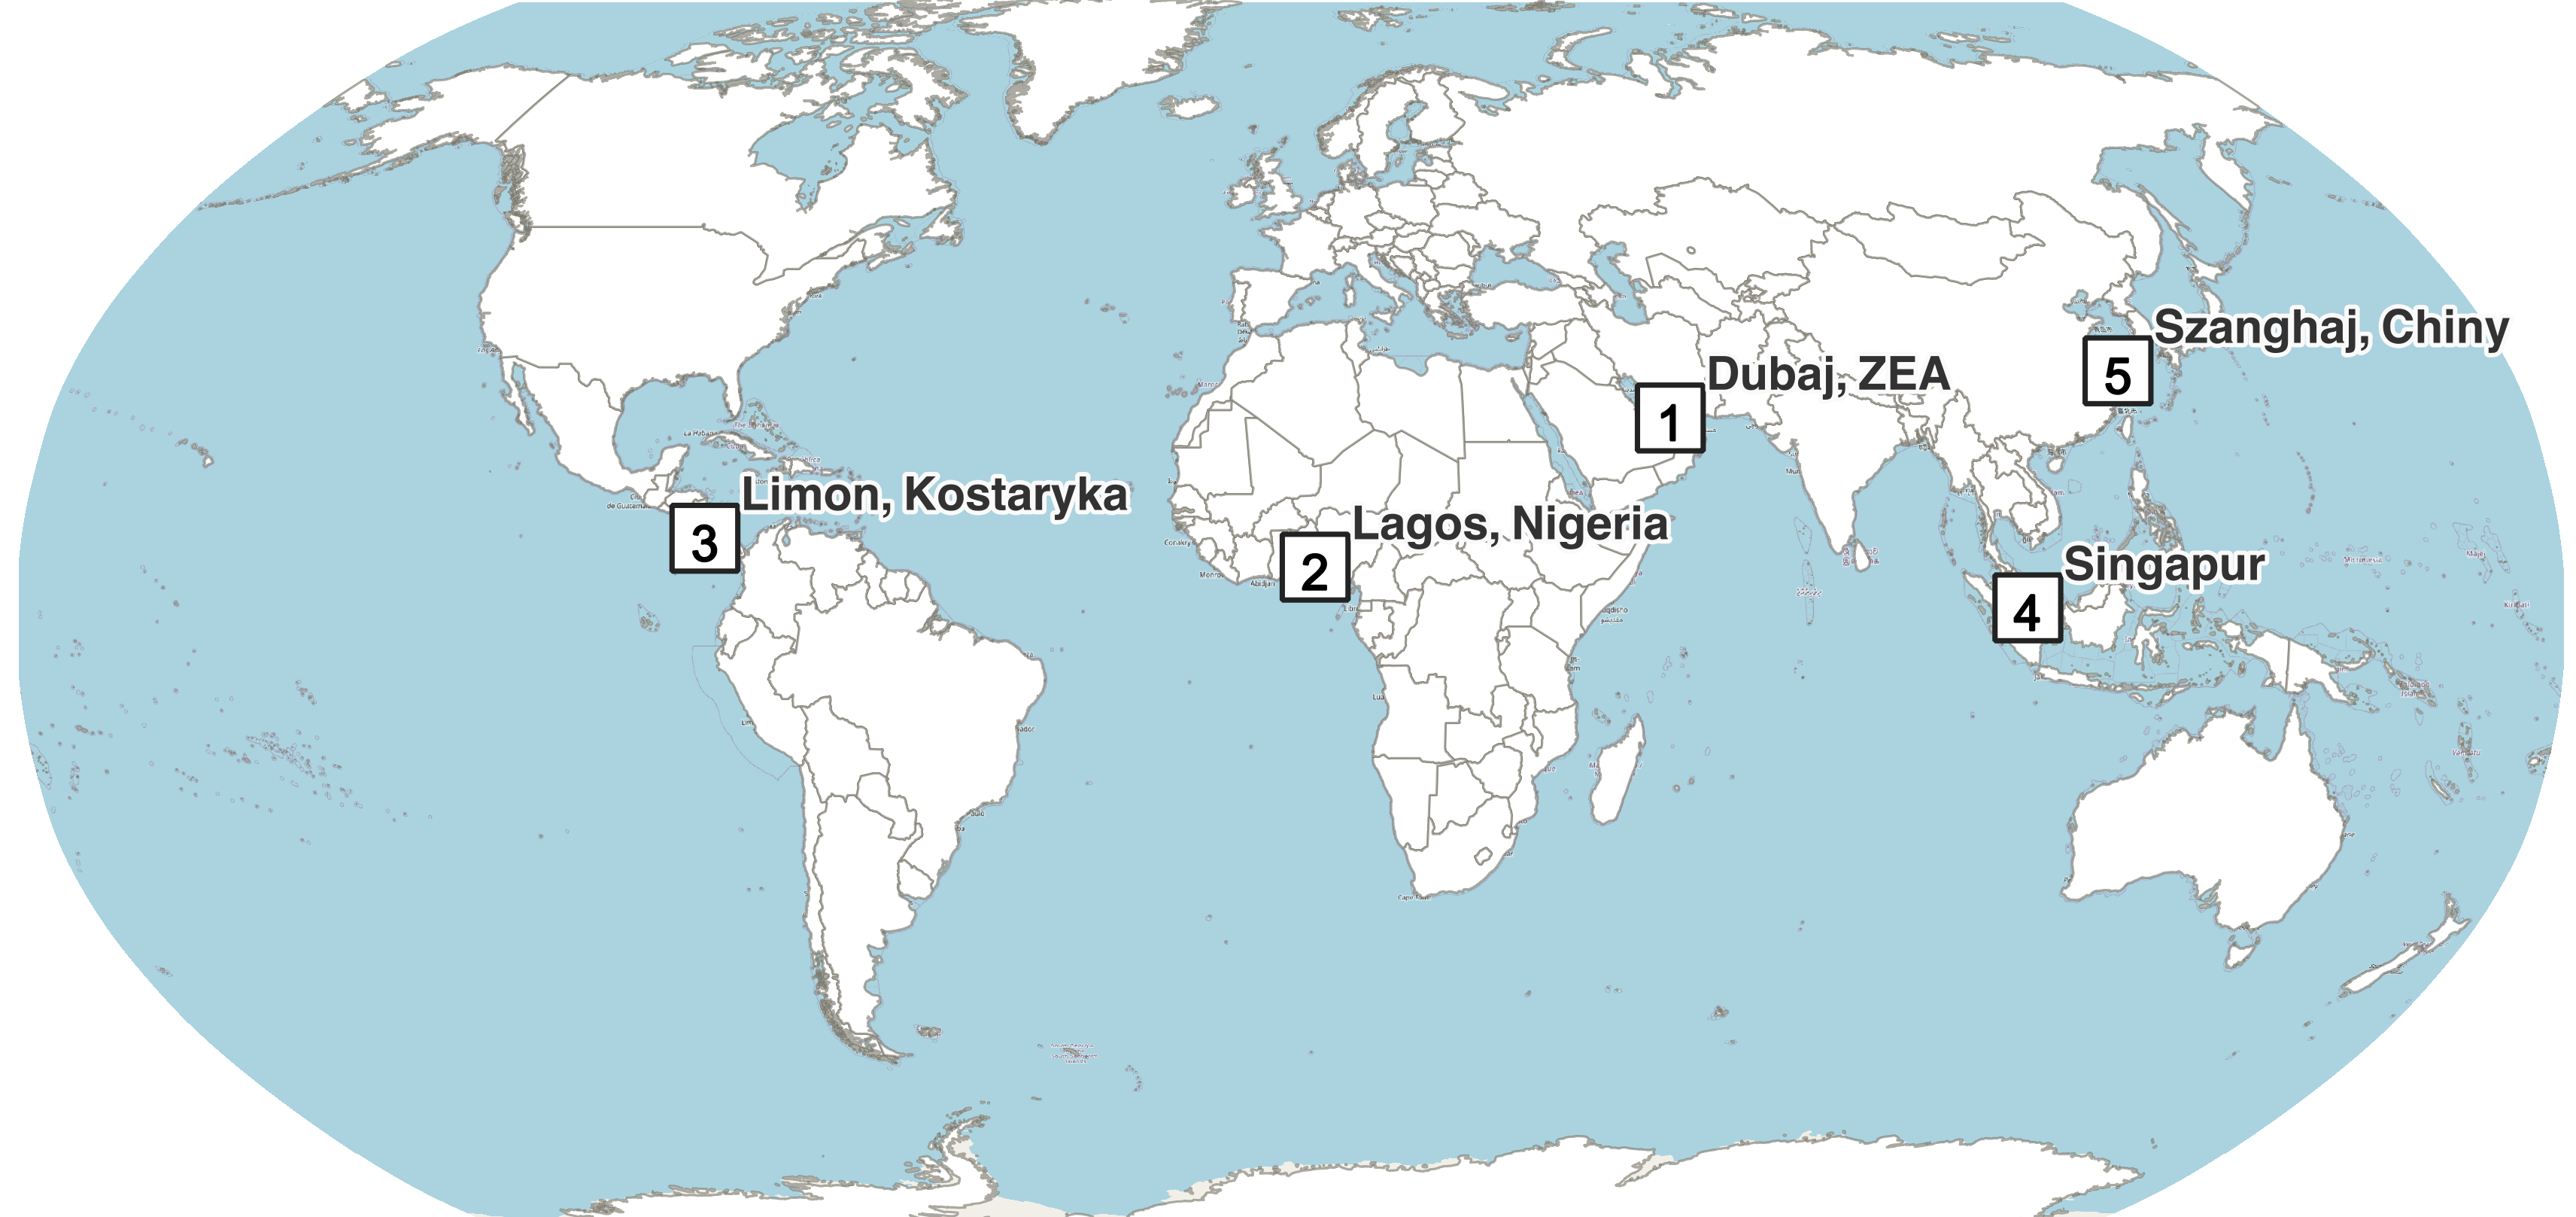
\includegraphics[width=1\textwidth,height=\textheight]{figures/aois3.png}

}

\caption{\label{fig-aois}Lokalizacja obszarów badań.}

\end{figure}

\begin{figure}[t]

{\centering 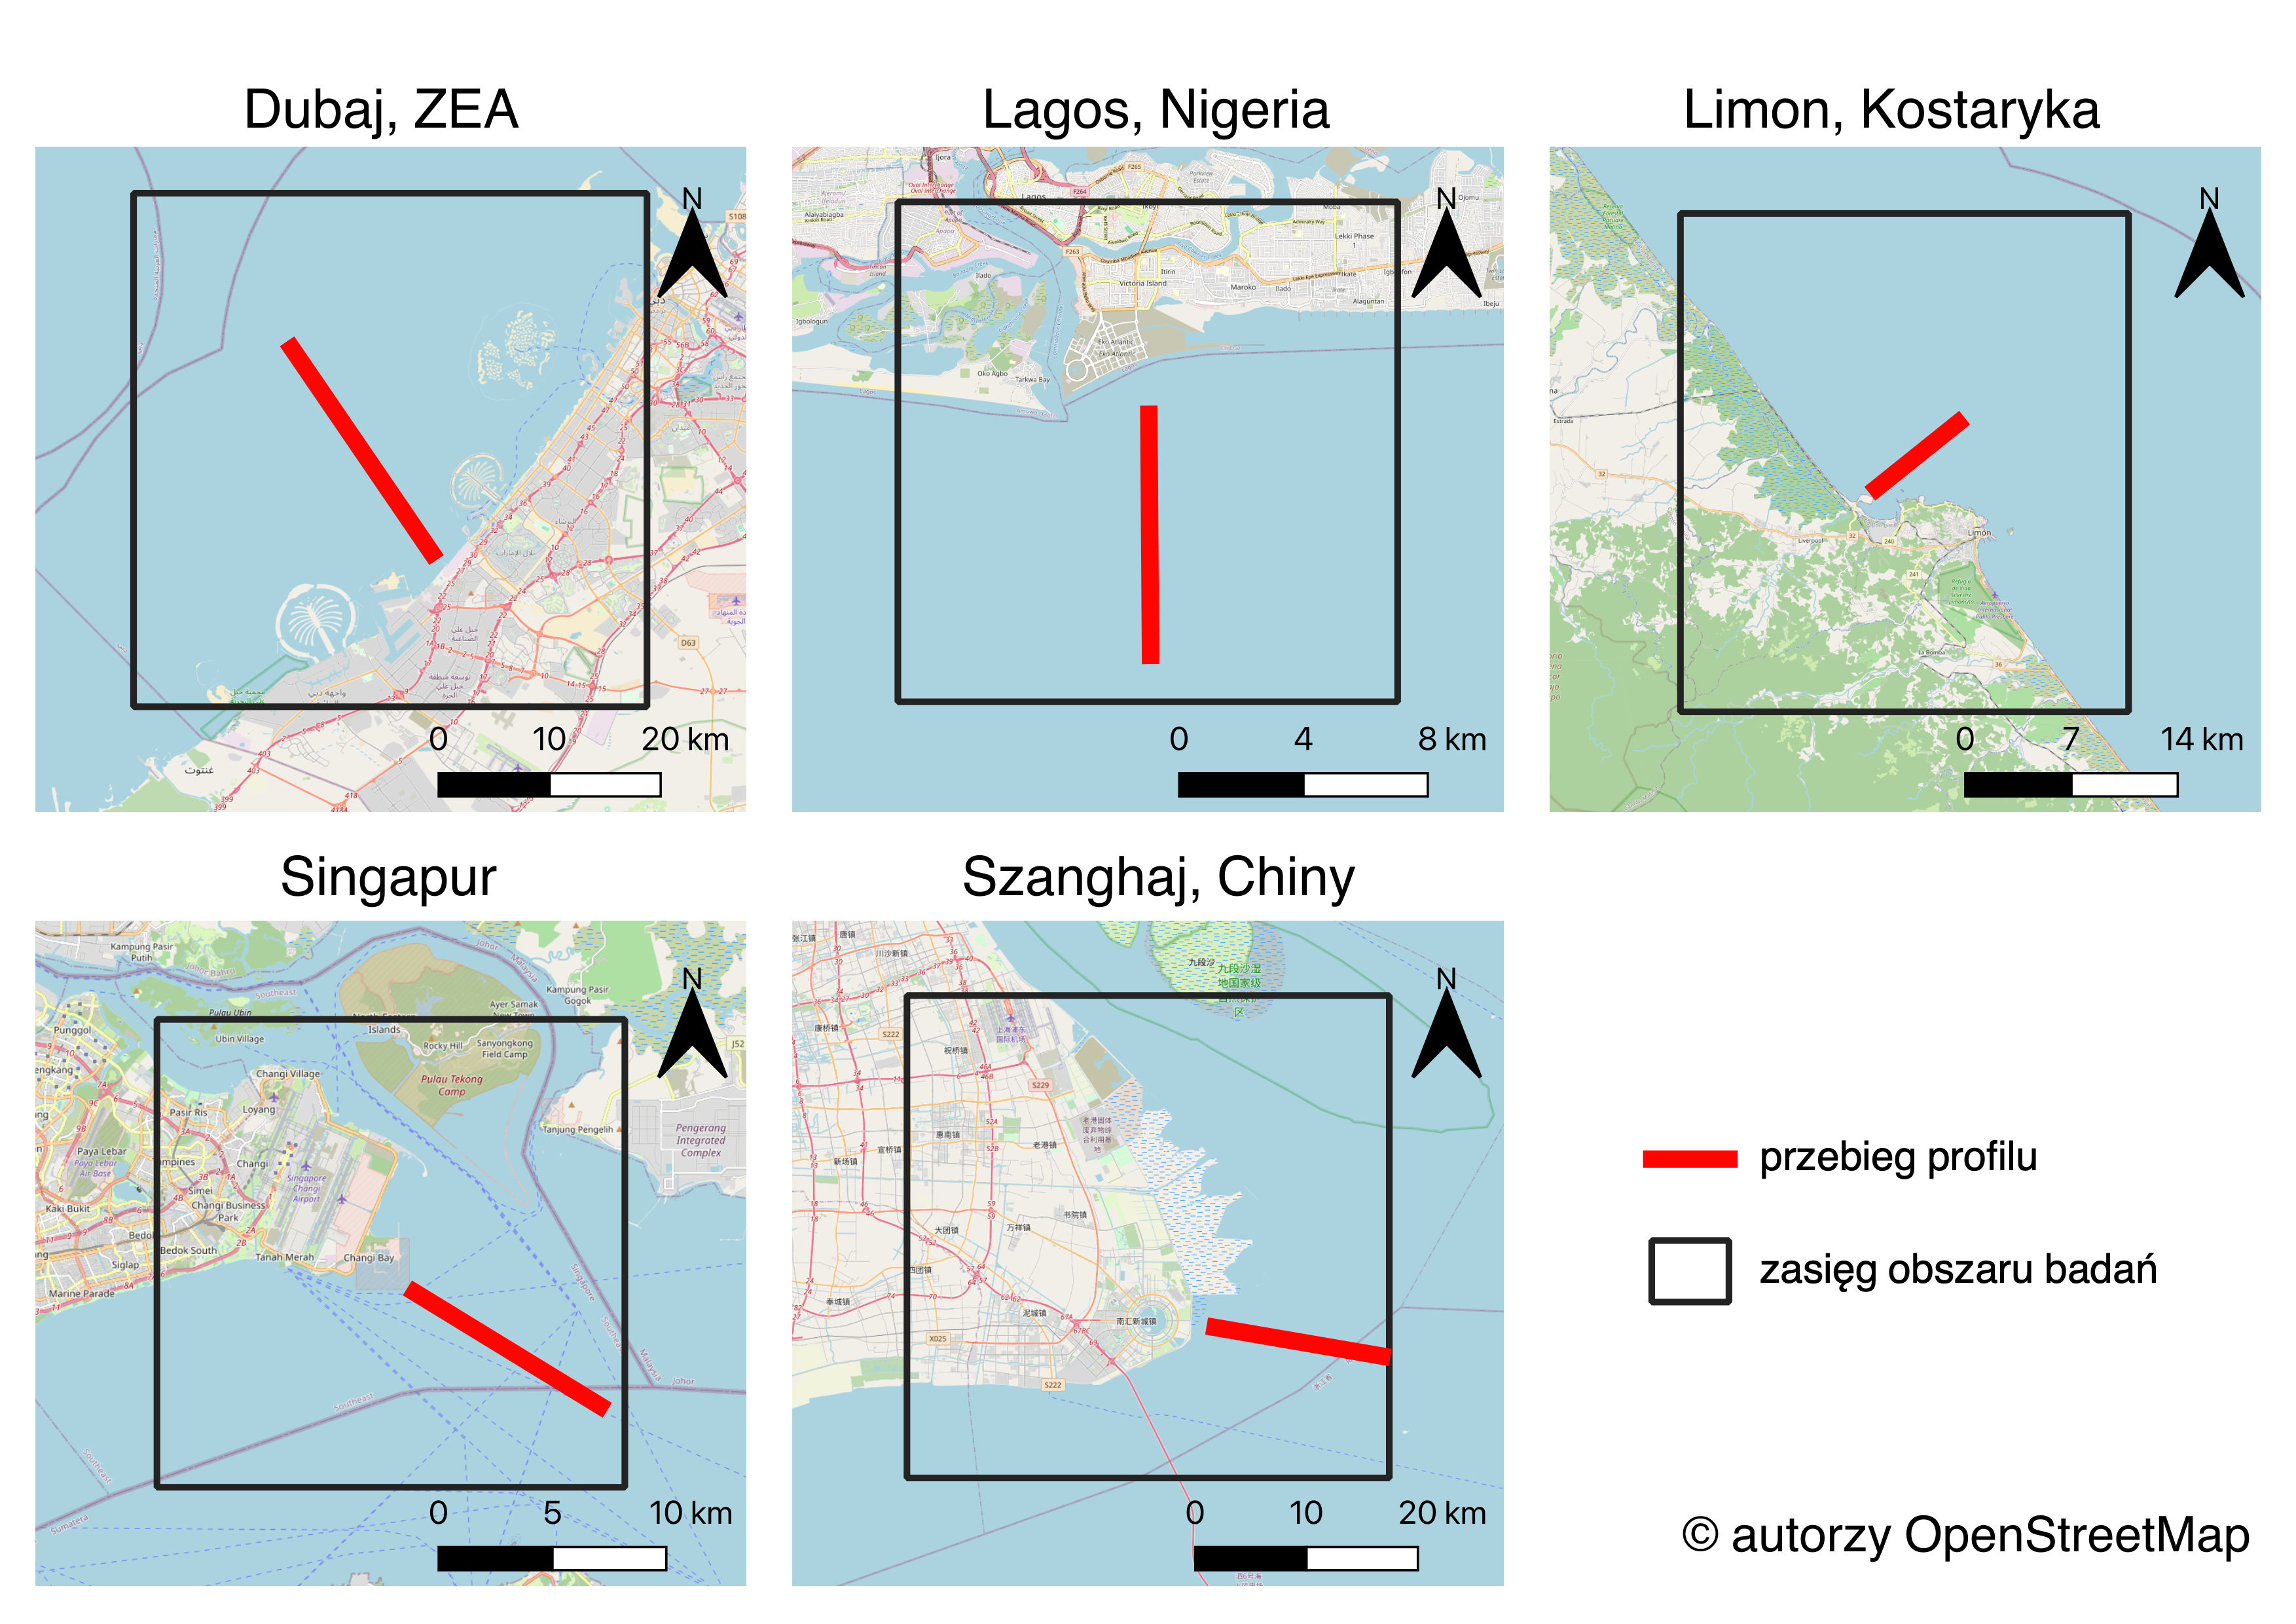
\includegraphics[width=1\textwidth,height=\textheight]{figures/aois_profiles.png}

}

\caption{\label{fig-aois_profiles}Zasięg przestrzenny obszarów badań i
przebieg profili.}

\end{figure}

\hypertarget{tbl-aois_info}{}
\begin{table}
\caption{\label{tbl-aois_info}Podstawowe informacje o obszarach badań, okresach prowadzenia prac,
wielkościach pozyskanych powierzchni i ich wykorzystaniu. }\tabularnewline

\centering
\begin{tabular}{l>{\raggedright\arraybackslash}p{2cm}>{\raggedright\arraybackslash}p{2cm}>{\raggedright\arraybackslash}p{2cm}l}
\toprule
obszar badań & początek prac & zakończenie prac & nowa powierzchnia & wykorzystanie\\
\midrule
Dubaj, ZEA & 2002 & 2010 & 20 km2 & turystyka\\
Lagos, Nigeria & 2009 & 2018 & 9 km2 & obszar mieszkalno-usługowy\\
Limon, Kostaryka & 2015 & 2018 & 0.4 km2 & terminal kontenerowy\\
Singapur & 1995 & 2003 & 30 km2 & lotnisko\\
Szanghaj, Chiny & 2003 & 2005 & 296 km2 & obszar mieszkalno-usługowy\\
\bottomrule
\end{tabular}
\end{table}

\hypertarget{dubaj-zjednoczone-emiraty-arabskie}{%
\section{Dubaj, Zjednoczone Emiraty
Arabskie}\label{dubaj-zjednoczone-emiraty-arabskie}}

\begin{figure}[t]

{\centering 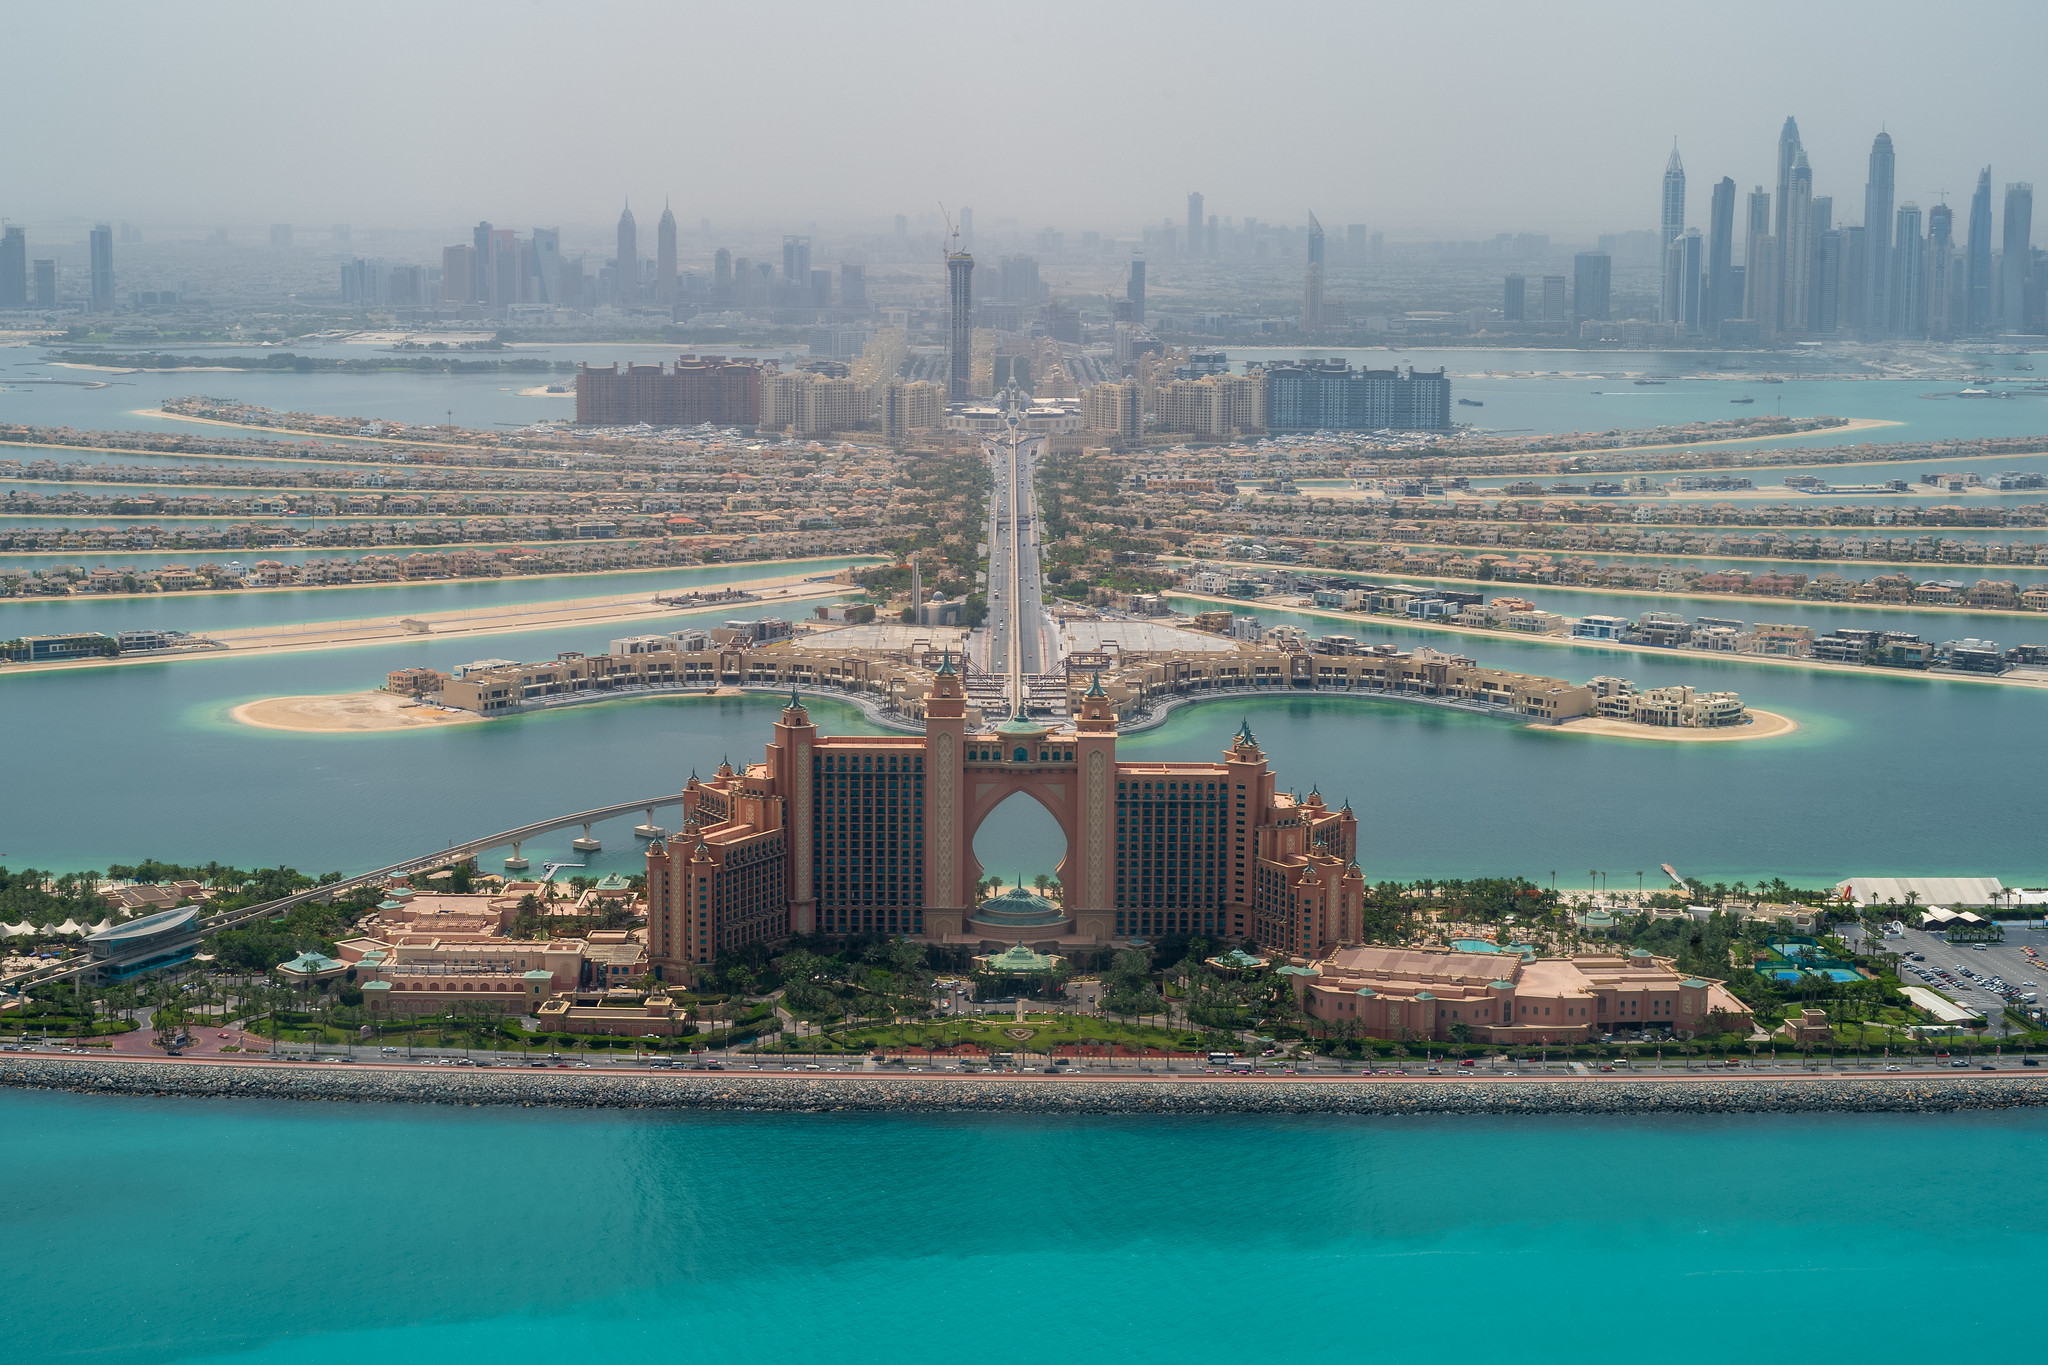
\includegraphics[width=1\textwidth,height=\textheight]{figures/dubai/dubai_aoi.jpg}

}

\caption{\label{fig-db_aoi}Hotel Atlantis, jeden z atrakcji Dubaju,
znajduje się na sztucznej wyspie Palm Jumeirah. (Źródło:
ckilger/flickr)}

\end{figure}

Na początku XX wieku rozpoczęto konstrukcje sztucznych wysp na wybrzeżu
Dubaju. Wynikało to ze wzrostu gospodarczego miasta w tym okresie
\autocite{gibling2013construction}. Nowe wyspy miały pełnić funkcje
turystyczne, będąc podłożem pod kompleksy hoteli, kurortów i atrakcji.
Do tych wysp zaliczyć można: Palm Jebel Ali, Palm Jumeirah, The World
Islands (Rycina~\ref{fig-db_aoi}). Łączna powierzchnia wysp wynosi 20
kilometrów kwadratowych. Mimo iż większość wysp udało się ukończyć, ich
dalszy rozwój został zahamowany w 2008 roku na skutek kryzysu
ekonomicznego \autocite{gupta2015futures}. W ramach pracy, badania na
obszarze Dubaju przeprowadzono w okresie od 2000 do 2012 roku.

\hypertarget{lagos-nigeria}{%
\section{Lagos, Nigeria}\label{lagos-nigeria}}

\begin{figure}[t]

{\centering 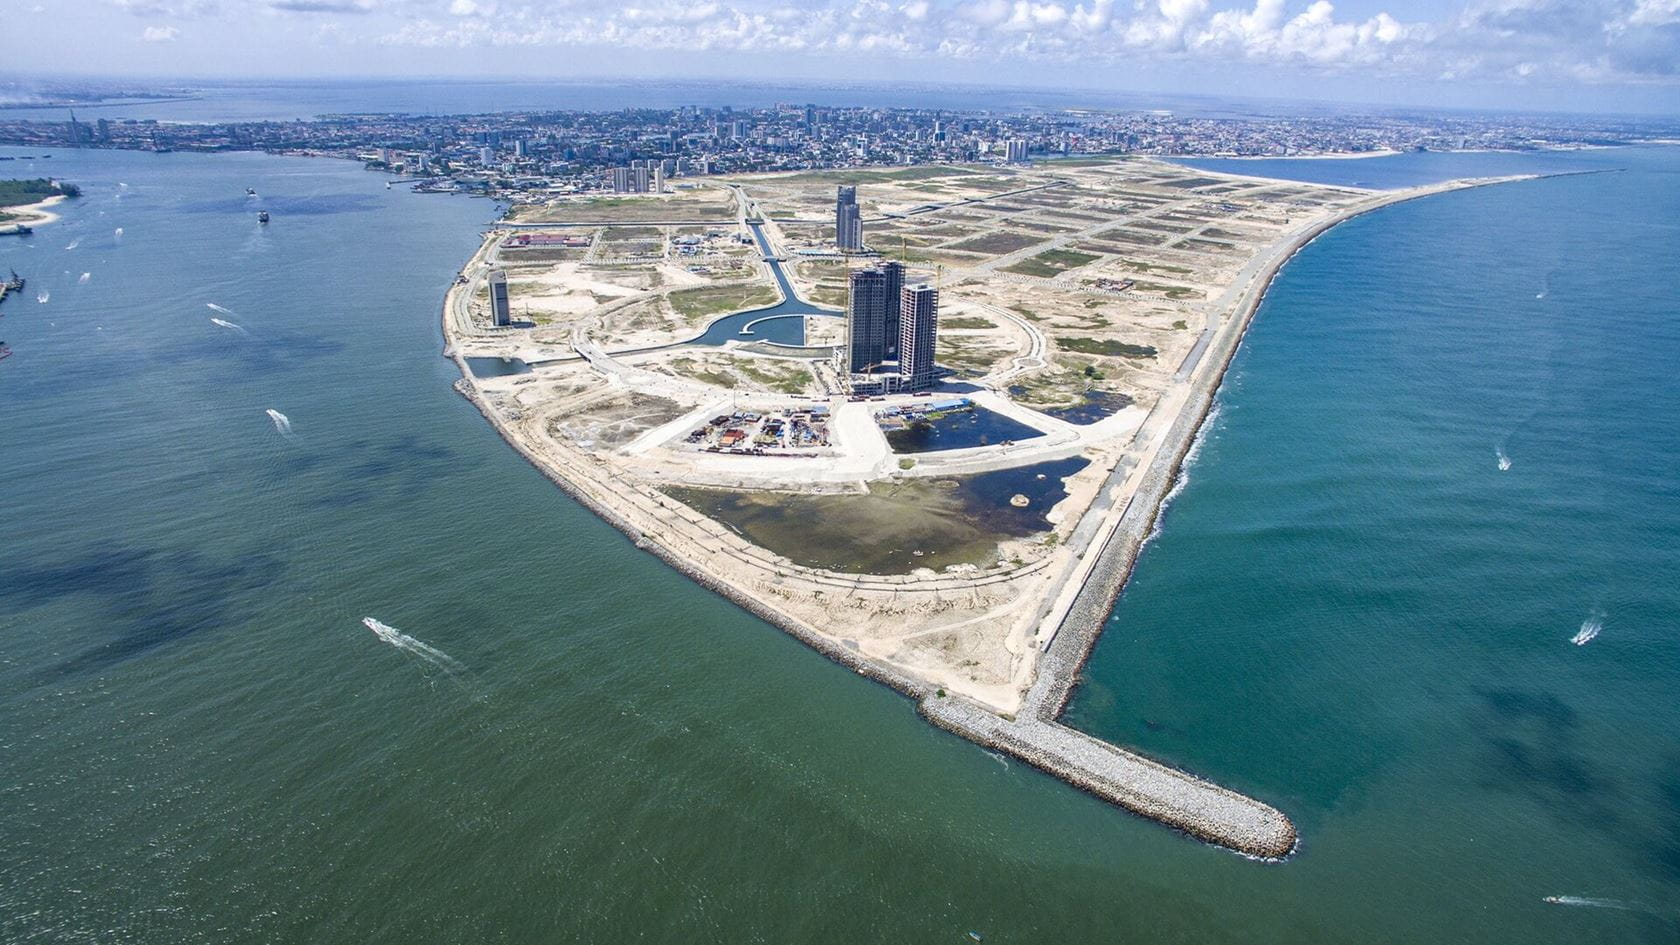
\includegraphics[width=1\textwidth,height=\textheight]{figures/nigeria/nigeria_aoi.jpeg}

}

\caption{\label{fig-lg_aoi}Eko Atlantic w 2020 roku na tle Lagosu.
(Źródło: South Energyx Nigeria Limited (SENL))}

\end{figure}

Lagos zmagał się z problemem wypłukiwania wybrzeża i wdzierania się
Zatoki Gwinejskiej wgłąb lądu. Rozwiązaniem problemu miał być projekt
Eko Atlantic, rozpoczęty w 2009 roku. Polegał on na konstrukcji nowego
lądu na wybrzeżu Lagosu. Pozwoliło to na odzyskanie 9 kilometrów
kwadratowych utraconej ziemi przez Nigerię, oraz jednoczesną konstrukcję
pasa umocnień \autocite{van2012lagos}. Mimo, iż konstrukcję nowego lądu
dla Eko Atlantic zakończono w 2018 roku, obszar ten nie jest dalej
zamieszkany. Cały czas mają miejsce prace nad budową infrastruktury,
budynków mieszkalnych i innych niezbędnych obiektów do funkcjonowania
Eko Atlantic. Eko Atlantic ma pełnić rolę nowego miasta oraz centrum
biznesowego, w którym mogłoby mieszkać 250 tysięcy mieszkańców
\autocite{omotosho2013new}. W ramach pracy, badania na obszarze Lagos
przeprowadzono od 2007 do 2020 roku (Rycina~\ref{fig-lg_aoi}).

\hypertarget{limon-kostaryka}{%
\section{Limon, Kostaryka}\label{limon-kostaryka}}

\begin{figure}[t]

{\centering 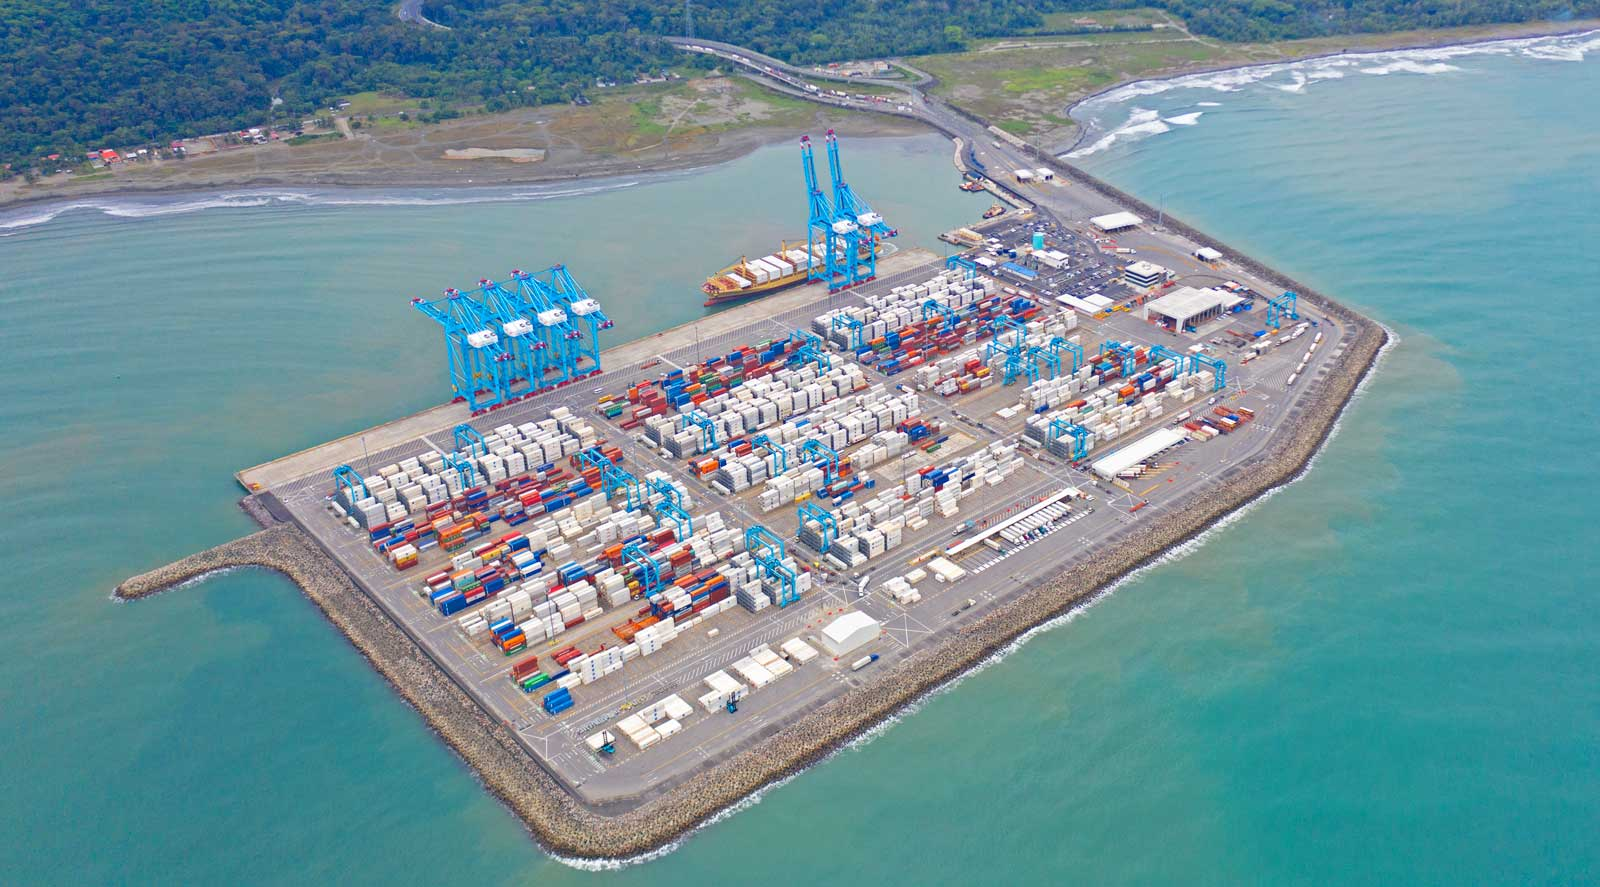
\includegraphics[width=1\textwidth,height=\textheight]{figures/costarica/costarica_aoi.jpg}

}

\caption{\label{fig-cr_aoi}Terminal kontenerowy Moin, Kostaryka, otwarty
w 2019 roku. (Źródło: APM Terminals)}

\end{figure}

Limon jest drugim największym miastem Kostaryki, pełniącym jednocześnie
rolę głównego portu morskiego kraju na Oceanie Atlantyckim. Kostaryka
posiada mocną pozycję na rynku eksportowym, będąc liderem na świecie w
ilości eksportowanych ananasów, oraz zajmując czwarte miejsce w ilości
eksportowanych bananów \autocite{notteboom2022port}. W celu rozwoju
gospodarki kraju i umocnienia pozycji na rynku Ameryki Łacińskiej, w
2015 roku rozpoczęto pracę nad budową nowego terminalu kontenerowego.
Terminal miał powstać na nowo utworzonej sztucznej wyspie obok miasta.
Prace ukończono w 2019 roku, oddając do użytku terminal kontenerowy Moin
o powierzchni 0.4 kilometra kwadratowego (Rycina~\ref{fig-cr_aoi}). W
przyszłości planowane są dalsze etapy rozbudowy terminalu, pozwalające
na obsługę większych kontenerowców i większej ilości towarów.
Wykorzystanie nowego terenu jest przemysłowe, służące jedynie obsłudze
terminalu portowego. W ramach pracy, badania na obszarze Limon
przeprowadzono w okresie od 2014 do 2020 roku.

\hypertarget{singapur}{%
\section{Singapur}\label{singapur}}

\begin{figure}[t]

{\centering 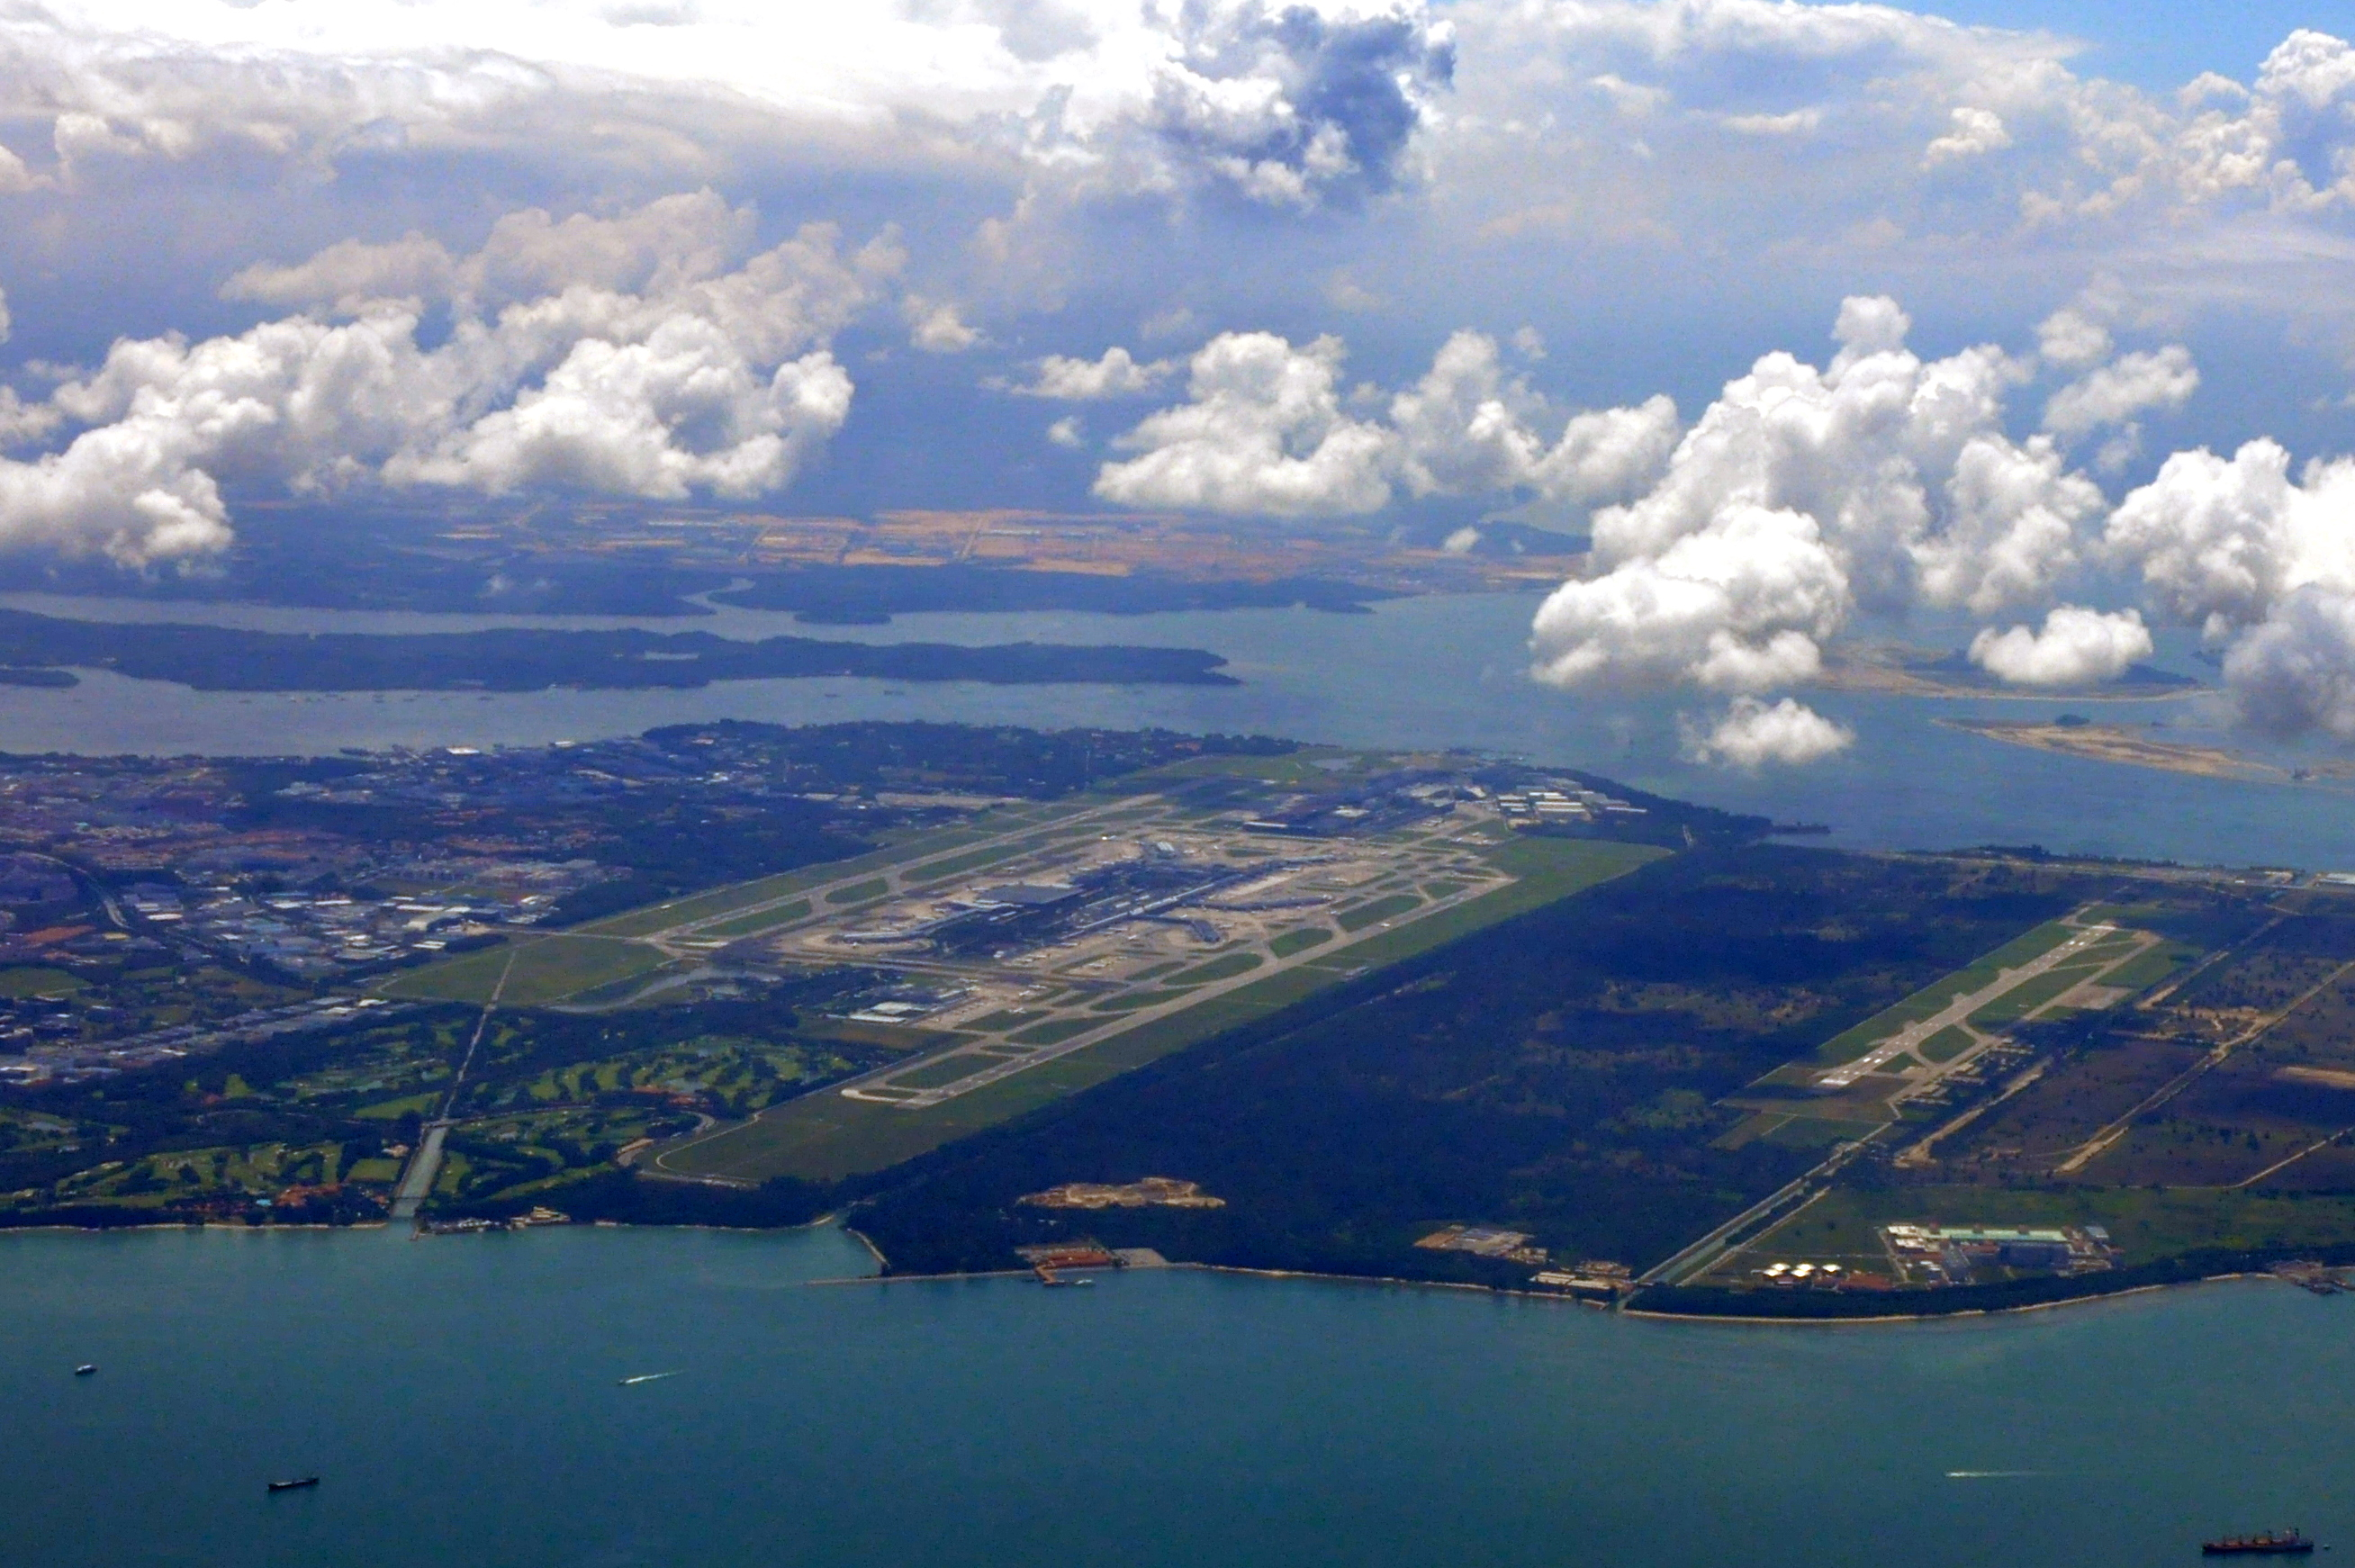
\includegraphics[width=1\textwidth,height=\textheight]{figures/singapore/singapore_aoi.jpeg}

}

\caption{\label{fig-sp_aoi}Utworzony ląd w Singapurze, na którym
znajdują się lotnisko Changi (lewo) i baza powietrzna Changi (prawo).
(Źródło: Pulkitsangal/Wikipedia)}

\end{figure}

Lotnisko Changi w Singapurze zostało otwarte w 1981 i pozwalało na
obsługę 12 milionów pasażerów rocznie \autocite{phang2003strategic}. W
1993 roku rozpoczęto w Singapurze Changi East Reclamation Project.
Projekt ten obejmował rozbudowę lotniska Changi o dodatkowe 30
kilometrów kwadratowych powierzchni (Rycina~\ref{fig-sp_aoi}). Nowy ląd
wykorzystano do rozbudowy infrastruktury lotniska oraz do zbudowania
nowych obiektów: baz powietrznych i morskich, oraz muzeum marynarki
wojennej kraju \autocite{arulrajah2009instrumentation}. W 2003 roku, w
którym zakończono projekt, lotnisko Changi w Singapurze było w stanie
obsłużyć rocznie 28 milionów pasażerów \autocite{phang2003strategic}. W
ramach pracy, badania na obszarze Singapuru przeprowadzono w okresie od
1991 do 2005 roku.

\hypertarget{szanghaj-chiny}{%
\section{Szanghaj, Chiny}\label{szanghaj-chiny}}

\begin{figure}[t]

{\centering 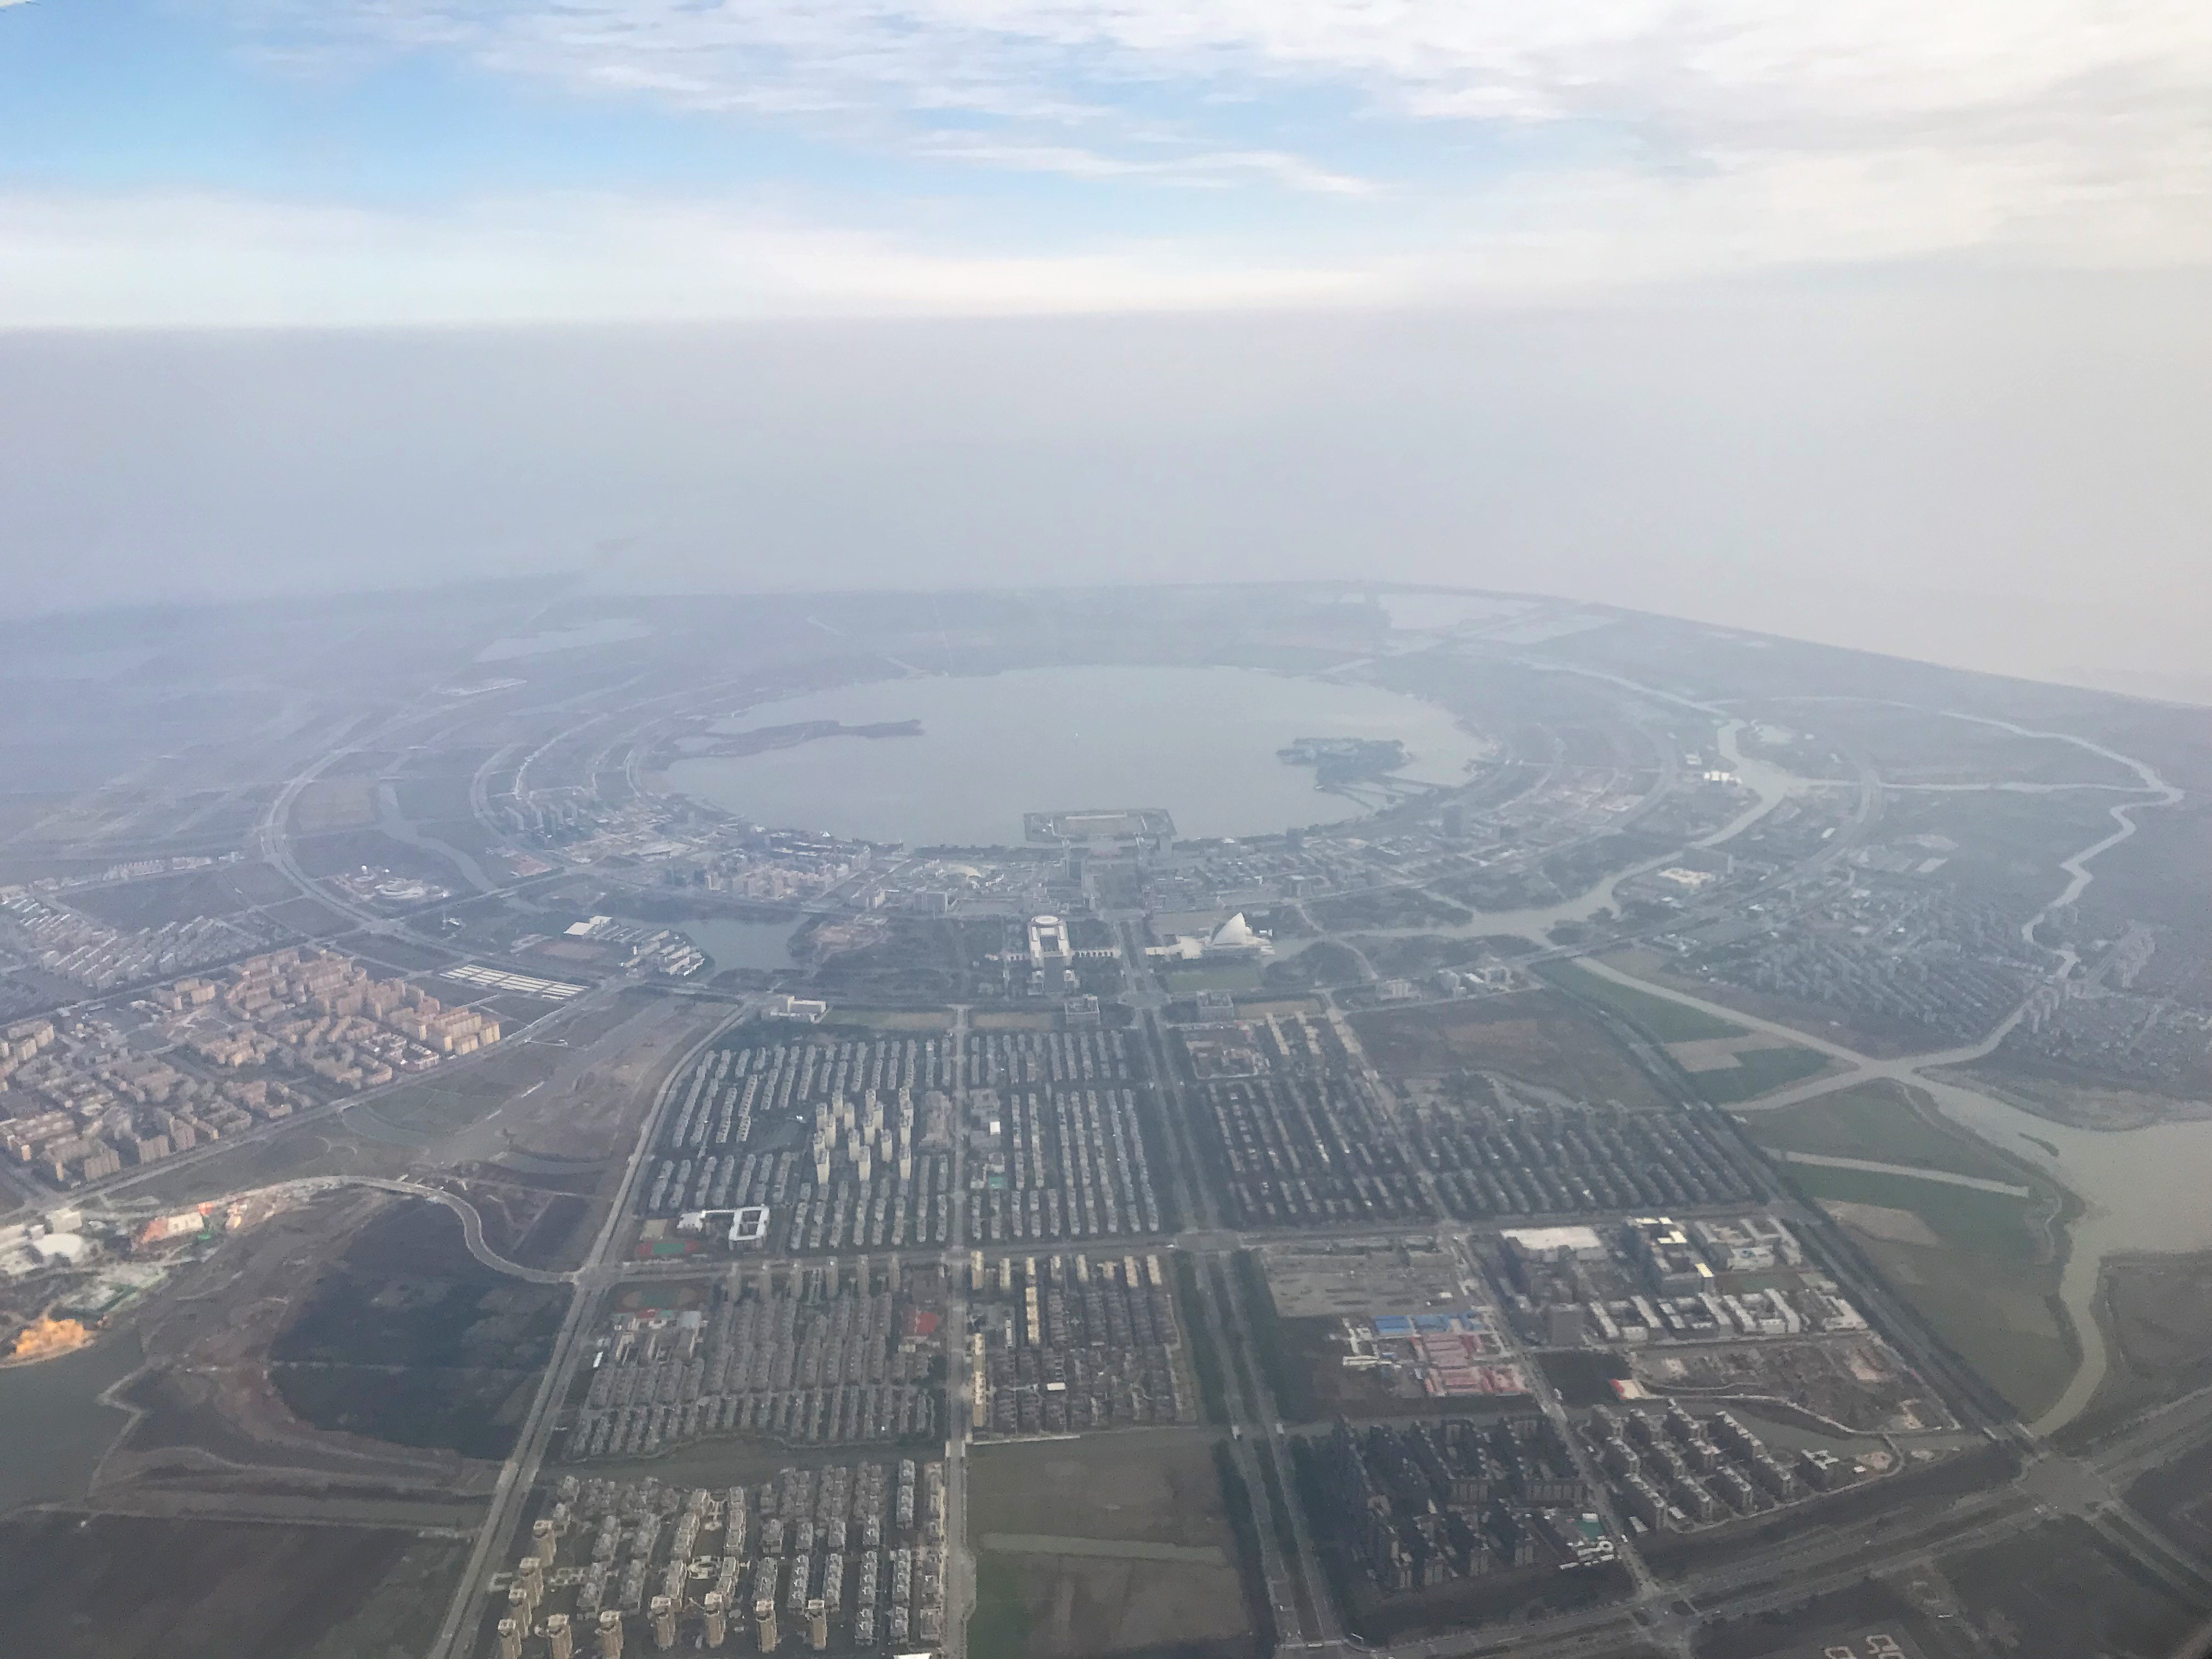
\includegraphics[width=1\textwidth,height=\textheight]{figures/china/china_aoi.jpg}

}

\caption{\label{fig-cn_aoi}Nanhui New City od strony zatoki Hangzhou,
rok 2018. źródło: MNXANL/Wikipedia}

\end{figure}

Szanghaj jest miastem o stale rosnącej liczbie ludności. Od 1990 do 2000
roku, populacja Szanghaju wzrosła z 8,6 do 14,2 milionów osób
\autocite{desaunited}. W celu zapewnienia miejsca zamieszkania dla stale
przybywającej ludności, rozpoczęto pracę nad rozbudową istniejących
dzielnic Szanghaju. Jednym z takich projektów było stworzenie Nanhui New
City, nowej dzielnicy Szanghaju w jej wschodniej części, nad zatoką
Hangzhou. Założeniem dzielnicy było stworzenie ośrodka, które nie będzie
jedynie częścią Szanghaju, a nowoczesnym miastem nadmorskim
\autocite{shi2016new}. Prace nad konstrukcją Nanhui New City rozpoczęto
w 2003 roku, planując zakończenie w 2020 roku. Celem lokalnego rządu
było stworzenie dzielnicy o powierzchni 296 kilometrów kwadratowych,
którą po zakończeniu prac mogłoby zamieszkiwać 800 tysięcy osób
(Rycina~\ref{fig-cn_aoi}). Mimo, iż prace w Nanhui New City trwały do
2020 roku, nowy ląd został zbudowany już w 2006 roku, a w 2010 roku
dzielnicę zamieszkiwało blisko 200 tysięcy osób \autocite{shi2016new}. W
ramach pracy, badania na obszarze Szanghaju przeprowadzono w zakresie
czasowym od 2000 do 2009 roku.

\bookmarksetup{startatroot}

\hypertarget{sec-materialy}{%
\chapter{Materiały}\label{sec-materialy}}

Do oceny stanu jakości wód, wykorzystano dane teledetekcyjne w postaci
obrazów satelitarnych. Tabela~\ref{tbl-data_info} zawiera szczegóły
odnośnie pozyskanych zdjęć. Wszystkie obrazy pochodzą z drugiego poziomu
programu Landsat Collection 2. W zależności od lat prowadzonych badań,
zdjęcia pochodzą z satelit Landsat 5, 7 lub 8. Obrazy pozyskano z
katalogu Planetary Computer od firmy Microsoft
\autocite{microsoft_open_source_2022_7261897}. Wszystkie zdjęcia mają
rozdzielczość przestrzenną 30 metrów.

Z pozyskanych zdjęć satelitarnych, do obliczenia wskaźników
spektralnych, wykorzystano kanały widzialne (czerwony, zielony,
niebieski) i bliskiej podczerwieni. Wykorzystany został również kanał
oceny jakości poszczególnych pikseli do wyboru jedynie obszarów
zaklasyfikowanych jako zbiorniki wodne bez pokrycia chmurami.

Tabela~\ref{tbl-data_info} zawiera również informacje o liczbie
dostępnych zdjęć dla obszarów badań, pozyskanych z Planetary Computer. W
przypadku Dubaju, Lagosu oraz Szanghaju, obszary badań były
wystarczająco duże, że ich obszar dla pojedynczych dni pokrywały dwa
zdjęcia satelitarne. Spowodowało to wzrost ilości dostępnych obrazów dla
tych obszarów. Dla Dubaju i Lagosu jednak, dwa zdjęcia dla tych samych
dni pokrywały się tak mocno, że dodatkowy obraz nie dostarczał nowych
informacji do obszaru badań. Ze wszystkich dostępnych zdjęć dla badanych
obszarów wybrano jedynie te, dla których procentowy udział ilości
pikseli bez wartości w całym obrazie nie przekroczył wartości progowej.
Wartość progowa zmieniała się dla każdego z obszarów, w zależności od
ilości obszarów lądowych znajdujących się w obszarze badań. Piksele
klasyfikowane jako ląd były wykluczane z analizy, w wyniku czego przy
dużym udziale lądu należało zwiększyć wartość progową braku wartości.
Oprócz lądów, chmury również wpływały na brak wartości na obrazie
satelitarnym. Przy dużym zachmurzeniu, liczba dostępnych pikseli dla
zbiorników wodnych malała, co skutkowało zmniejszeniem przydatności
takiego zdjęcia do badań.

Oprócz zdjęć satelitarnych, w pracy wykorzystano również dane o
głębokości zbiorników wodnych ze zbioru GEBCO\_2023 Grid
\autocite{gebco_2023}. Każda komórka rastra zawiera informacje o
głębokości w metrach. Dane o batymetrii zostały wykorzystane do zbadania
zmian wartości wskaźników jakości wód wzdłuż profilów, biegnących od
nowych lądów wgłąb zbiorników wodnych. Pozwoliło to na ocenę zmiany
jakości wód wraz ze zwiększaniem odległości od lądu oraz wraz ze
zwiększaniem głębokości.

\hypertarget{tbl-data_info}{}
\begin{table}
\caption{\label{tbl-data_info}Informacje o wykorzystanych danych oraz długości profilu. W tabeli
podano lata, dla których pozyskano obrazy satelitarne. Zawarto także
ilość dostępnych zdjęć, oraz ile z nich zostało wykorzystane w
badaniach. Umieszczono również informacje o rodzaju satelity, które
wykonały zdjęcia. W tabeli zawarto również długość profilu w metrach,
wzdłuż którego próbkowano wartości wskaźników spektralnych oraz
głębokości zbiornika. }\tabularnewline

\centering
\begin{tabular}{lll>{\raggedright\arraybackslash}p{2cm}>{\raggedright\arraybackslash}p{2cm}l}
\toprule
obszar badań & satelita & okres badań & liczba dostępnych zdjęć & liczba wybranych zdjęć & długość profilu\\
\midrule
Dubaj, ZEA & Landsat 7 & 2002 - 2012 & 410 & 45 & 22149 m\\
Lagos, Nigeria & Landsat 7 i 8 & 2007 - 2020 & 465 & 51 & 7654 m\\
Limon, Kostaryka & Landsat 8 & 2014 - 2020 & 316 & 27 & 6853 m\\
Singapur & Landsat 5 i 7 & 1993 - 2005 & 337 & 46 & 9479 m\\
Szanghaj, Chiny & Landsat 7 & 2000 - 2008 & 759 & 39 & 15134 m\\
\bottomrule
\end{tabular}
\end{table}

\bookmarksetup{startatroot}

\hypertarget{sec-wyniki}{%
\chapter{Wyniki}\label{sec-wyniki}}

Rozdział ten poświęcony jest analizie wartości wskaźników spektralnych i
próbie odpowiedzi na pytanie, czy tworzenie nowych lądów wpływa na
jakość wód? Wskaźniki spektralne zostały obliczone dla każdego obrazu
satelitarnego, wybranego według podanego kryterium
(Rozdział~\ref{sec-metody} zawiera dokładny opis tego procesu).
Obserwacja zmian stanu jakości wód polegała na zestawieniu wartości
poszczególnych wskaźników z okresu trwania prac nad tworzeniem nowych
lądów, z wartościami tych samych wskaźników przed rozpoczęciem prac.
Dodatkowo, wartości wskaźników obliczonych na obrazach z etapu trwania
prac i przed ich rozpoczęciem zestawiono także z obrazami wykonanymi po
zakończeniu prac, w celu obserwacji możliwych długofalowych efektów
tworzenia nowych lądów na stan jakości wód. Rozdział ten podzielony jest
na podrozdziały, poświęcone każdemu obszarowi badań z osobna.

Wzrost wartości wszystkich wskaźników interpretowany jest jako wzrost
intensywności obserwowanego zjawiska. Oznacza to, że wzrost wartości
wskaźników Bow06 i Chip09 jest interpretowany jako wzrost stężenia
zawiesiny w wodzie. Wzrost stężenia zawiesiny wskazuje na zwiększenie
mętności wody. Zjawisko te interpretowane jest jako negatywne,
pogarszające stan jakości wód.

W przypadku chlorofilu a, w pracy nie zawarto opinii o negatywnym czy
pozytywnym wpływie zmian tego parametru na jakość wód. Zarówno wzrost
stężenia chlorofilu a jak i jego spadek może być utożsamiany z
pogorszeniem stanu wód \autocite{dembowska2021use}. Wzrost stężenia
chlorofilu a wskazuje na wzrost biomasy fitoplanktonu, co prowadzi do
przekwitu glonów. Odnotowanie spadku stężenia chlorofilu a może
świadczyć o zaniku fitoplanktonu, co prowadzi do ograniczenia
dostępności pokarmu dla organizmów wodnych. W pracy skupiono się na
obserwacji zmian stężenia chlorofilu a między etapami prac. Wielkość
tych zmian może być sygnałem potencjalnego wpływu tworzenia nowych lądów
na stan jakości wód.

Podrozdziały zawierają wybrane ryciny, przedstawiające wpływ procesów
tworzenia nowych lądów na jakość wód. Pozostałe ryciny, utworzone w
ramach pracy, zostały umieszczone w rozdziale z załącznikami.

\hypertarget{dubaj-zjednoczone-emiraty-arabskie-1}{%
\section{Dubaj, Zjednoczone Emiraty
Arabskie}\label{dubaj-zjednoczone-emiraty-arabskie-1}}

\hypertarget{tbl-db_stats}{}
\begin{table}
\caption{\label{tbl-db_stats}Średnie wartości wskaźników jakości wody dla Dubaju z podziałem na dwie
grupy parametrów jakości wód (chlorofil a i zawiesina) oraz na trzy
etapy prac (przed, w trakcie i po zakończeniu). W tabeli zawarto również
p-value z testu Kruskala-Wallisa, sprawdzającego istotność statystyczną
zmian średnich wartości wskaźników między etapami prac. }\tabularnewline

\centering
\begin{tabular}{lrrrr}
\toprule
  & przed (2000-2001) & w trakcie (2002-2010) & po (2011-2012) & p-value\\
\midrule
\addlinespace[0.3em]
\multicolumn{5}{l}{\textbf{chlorofil a}}\\
\hspace{1em}SABI & -0.059 & -0.061 & -0.067 & 0.098\\
\hspace{1em}FLH Blue & 0.006 & 0.007 & 0.007 & 0.106\\
\addlinespace[0.3em]
\multicolumn{5}{l}{\textbf{zawiesina}}\\
\hspace{1em}Bow06 & 0.705 & 0.764 & 0.712 & 0.153\\
\hspace{1em}Chip09 & 0.577 & 0.635 & 0.568 & 0.170\\
\bottomrule
\end{tabular}
\end{table}

Obserwując zmiany wartości parametrów jakości wody, odnotowano wpływ
tworzenia nowych lądów na jakość wód w Dubaju. Tabela~\ref{tbl-db_stats}
przedstawia średnie wartości poszczególnych wskaźników dla każdego z
etapów pracy. Średnia wartość wskaźnika SABI była niższa w etapie
trwania prac niż w okresie przed rozpoczęciem prac. Wskazuje to na
zmniejszenie stężenia chlorofilu a na obszarze badań po rozpoczęciu
prac. Drugi wskaźnik wykrywający chlorofil a, FLH Blue, odnotował
natomiast wzrost średnich wartości po rozpoczęciu prac. Średnie wartości
wskaźnika SABI po zakończeniu prac były jeszcze niższe niż podczas
trwania prac. Może to świadczyć o długofalowych skutkach konstrukcji
nowych lądów na jakość wód. Biorąc pod uwagę przeznaczenie nowego lądu,
można przypuszczać o wpływie ruchu turystycznego na dalszą degradację
pobliskich wód.

Obydwa wskaźniki wykrywające zawiesinę w wodzie wskazują na wzrost
stężenia zawiesiny podczas trwania prac tworzenia nowego lądu, w
porównaniu do stanu przed rozpoczęciem budowy. Proces tworzenia nowych
lądów w Dubaju poskutkował zwiększeniem mętności wody i pogorszeniem
stanu jakości pobliskich wód. Po zakończeniu prac, średnie wartości
wskaźników badających występowanie zawiesiny zmalały do poziomu
bliskiemu stanu przed rozpoczęciem prac.

\begin{figure}[t]

{\centering 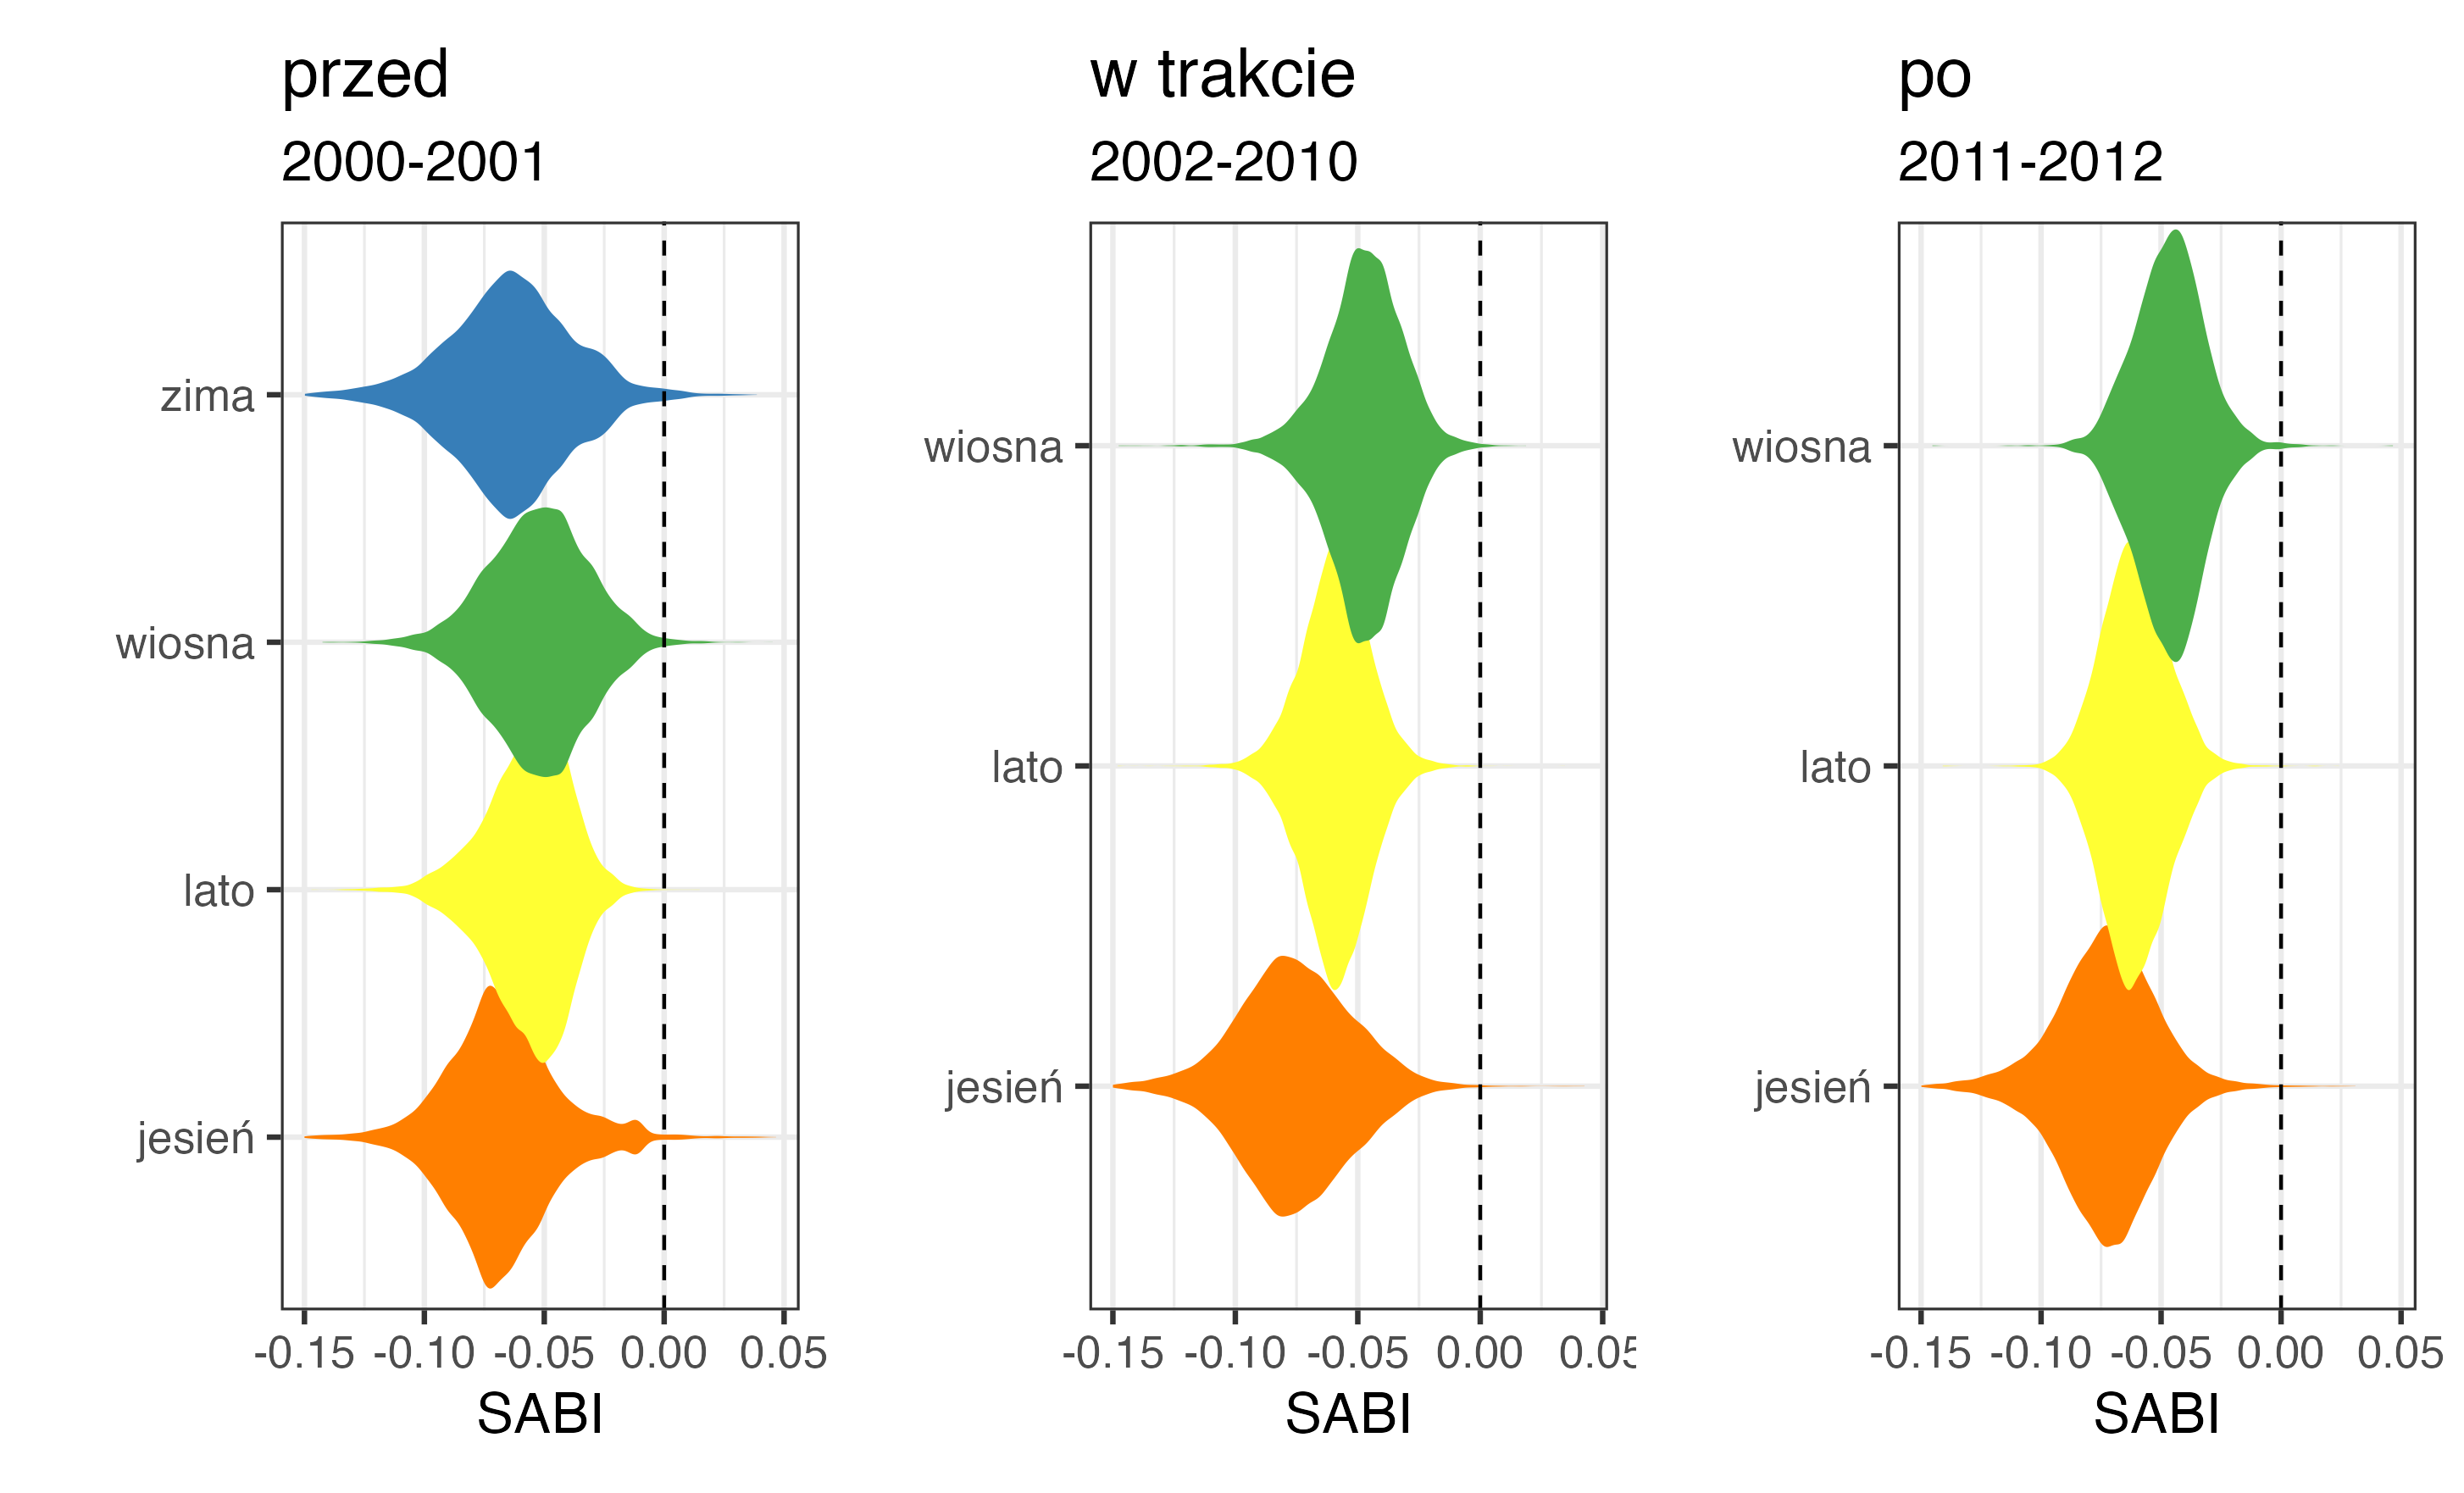
\includegraphics[width=6.25in,height=\textheight]{figures/dubai/sabi_violin.png}

}

\caption{\label{fig-db_sabi_violin}Rozkład stężenia chlorofilu a dla
Dubaju na przykładzie wskaźnika SABI, z podziałem na trzy etapy prac:
przed rozpoczęciem, w trakcie i po zakończeniu prac, oraz na cztery pory
roku.}

\end{figure}

Oprócz zmian średnich wartości parametrów jakości wód, zmianom uległy
również rozkłady wartości. Rycina~\ref{fig-db_sabi_violin} przedstawia
rozkłady wartości chlorofilu a w wodzie, bazując na wskaźniku SABI.
Wskaźniki obliczone podczas trwania prac wykazują mniejsze rozproszenie
wokół średniej niż wskaźniki obliczone przed rozpoczęciem prac. Jest to
widoczne szczególnie na wskaźnikach obliczonych przy pomocy zdjęć,
pochodzących z letniego sezonu. Oznacza to, że proces tworzenia nowych
lądów wpłynął na jakość wód i sprawił, że na obszarze badań w Dubaju
stężenie chlorofilu a stało się bardziej jednorodne. Przy jednoczesnym
spadku stężenia chlorofilu a wskazuje to na wpływ procesów lądotwórczych
na jakość wód, przez które chlorofilu a w wodzie jest mniej na całym
obszarze badań, a nie jedynie przy nowym terenie lądowym.

\begin{figure}[t]

{\centering 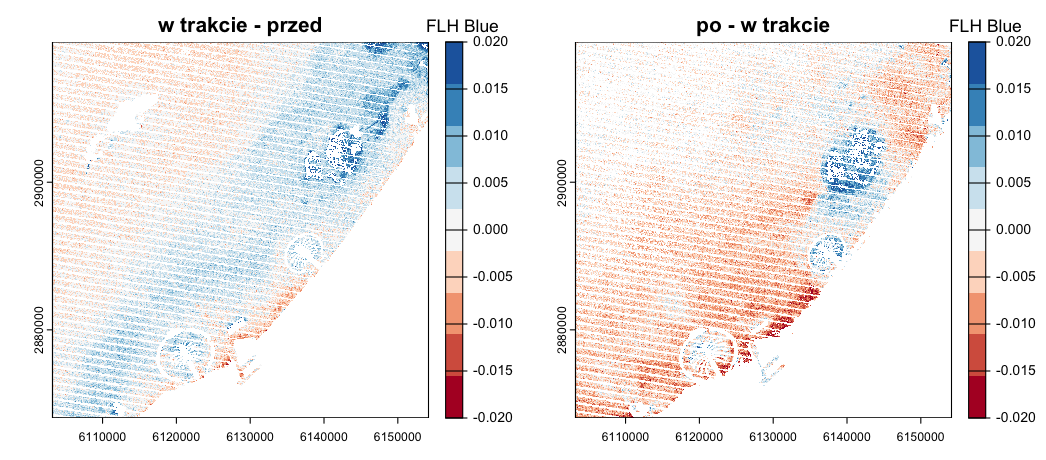
\includegraphics[width=6.25in,height=\textheight]{figures/dubai/flhblue_diff.png}

}

\caption{\label{fig-db_flhblue_diff}Mapy różnic występowania chlorofilu
a dla Dubaju, z wykorzystaniem wskaźnika FLH Blue. Rycina po lewej
przedstawia różnice między wskaźnikami, obliczonymi w trakcie trwania i
przed rozpoczęciem prac (sierpień 2007 i 2000). Rycina po prawej
przedstawia różnice między wskaźnikami, obliczonymi po zakończeniu prac
i w trakcie ich trwania (listopad 2011 i 2002).}

\end{figure}

Rycina~\ref{fig-db_flhblue_diff} ukazuje zmiany w występowaniu
chlorofilu a między wybranymi etapami prac. Lewa rycina przedstawia
różnice wartości między wskaźnikami obliczonymi w trakcie prowadzenia
prac a wskaźnikami obliczonymi przed rozpoczęciem prac. Wartości
dodatnie świadczą o wzroście ilości chlorofilu a podczas trwania prac w
porównaniu do stanu przed rozpoczęciem, a wartości ujemne wskazują na
spadek ilości chlorofilu a wraz z rozpoczęciem prac. Na mapie widoczny
jest spadek stężenia chlorofilu a na południu obszaru badań, czyli tuż
przy wybrzeżu i nowym lądzie. Rycina po prawej stronie przedstawia
różnice między stężeniem chlorofilu a po zakończeniu prac a stężeniem
wykrytym w trakcie. Większość obszaru badań wskazuje na ujemne wartości,
co oznacza spadek stężenia chlorofilu a po zakończeniu prac.

\begin{figure}[t]

{\centering 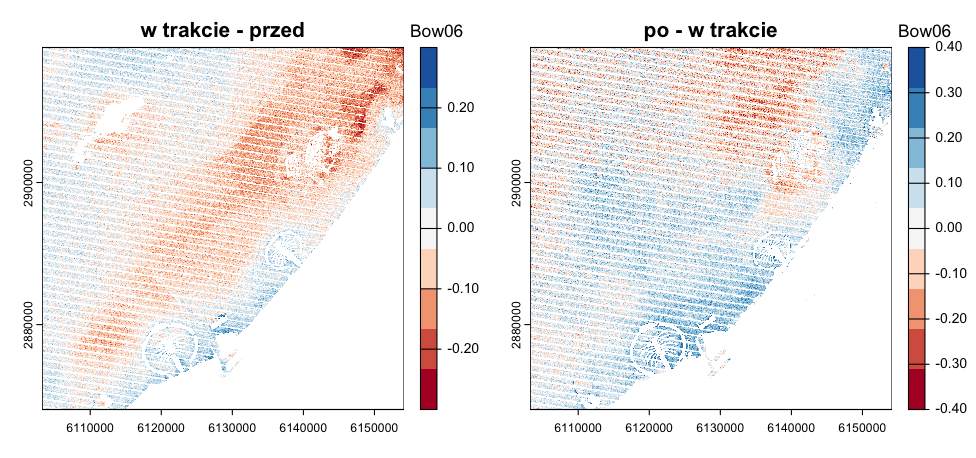
\includegraphics[width=6.25in,height=\textheight]{figures/dubai/bow_diff.png}

}

\caption{\label{fig-db_bow_diff}Mapy różnic występowania zawiesiny dla
Dubaju, z wykorzystaniem wskaźnika Bow06. Rycina po lewej przedstawia
różnice między wskaźnikami, obliczonymi w trakcie trwania i przed
rozpoczęciem prac (sierpień 2007 i 2000). Rycina po prawej przedstawia
różnice między wskaźnikami, obliczonymi po zakończeniu prac i w trakcie
ich trwania (listopad 2011 i 2002).}

\end{figure}

Rycina~\ref{fig-db_bow_diff} bada podobne różnice między wybranymi
etapami prac, jednak pod kątem obecności zawiesiny w wodzie. Lewa mapa
wskazuje na najwyższy wzrost mętności wody przy wybrzeżu, w miejscu
prowadzenia prac. Oznacza to, że konstrukcja nowych lądów przyczyniła
się do zwiększenia mętności wody przy wybrzeżu Dubaju. Stężenie
zawiesiny spadło natomiast wraz z oddalaniem się od wybrzeża. Dla
drugiej mapy, obszar wzrostu stężenia zawiesiny poszerzył się, w
porównaniu do pierwszej ryciny. Świadczy to o negatywnym skutku
tworzenia nowych lądów, który spowodował spadek jakości wody na większym
obszarze niż prowadzono prace.

Zmiany średnich wartości chlorofilu a w Dubaju były najmniejsze spośród
wszystkich obszarów badań, co może zostać odebrane jako niski wpływ
tworzenia nowych lądów na stan jakości wód. Odnotowane zostały natomiast
zmiany w rozkładzie wartości stężeń chlorofilu a. Podczas trwania prac,
wartości stężenia chlorofilu a były bardziej jednorodne niż przed
rozpoczęciem konstrukcji nowego lądu. Zauważono również największy
spadek stężenia chlorofilu a w pobliżu miejsca tworzenia nowego lądu, w
porównaniu do pozostałego obszaru badań. Dodatkowo, zaobserwowano
zwiększenie stężenia zawiesiny w wodzie podczas etapu konstrukcji lądu
względem stanu przed pracami. Wzrost mętności wody mógł wpłynąć
negatywnie na stan jakości wód w Dubaju. Proces konstrukcji nowego lądu
albo jego forma użytkowania mogły przyczynić się do dalszej degradacji
jakości wód w Dubaju. Potwierdzenie ciągłej degradacji wymagałoby
dalszej obserwacji zmian parametrów jakości wód po zakończeniu prac.
Zmiany średnich wartości wskaźników między etapami prac nie wykazały
istotności statystycznej.

\hypertarget{lagos-nigeria-1}{%
\section{Lagos, Nigeria}\label{lagos-nigeria-1}}

\hypertarget{tbl-lg_stats}{}
\begin{table}
\caption{\label{tbl-lg_stats}Średnie wartości wskaźników jakości wody dla Lagos z podziałem na dwie
grupy parametrów jakości wód (chlorofil a i zawiesina) oraz na trzy
etapy prac (przed, w trakcie i po zakończeniu). W tabeli zawarto również
p-value z testu Kruskala-Wallisa, sprawdzającego istotność statystyczną
zmian średnich wartości wskaźników między etapami prac. }\tabularnewline

\centering
\begin{tabular}{lrrrr}
\toprule
  & przed (2007-2008) & w trakcie (2009-2018) & po (2019-2020) & p-value\\
\midrule
\addlinespace[0.3em]
\multicolumn{5}{l}{\textbf{chlorofil a}}\\
\hspace{1em}SABI & -0.081 & -0.035 & -0.044 & 0.132\\
\hspace{1em}FLH Blue & 0.006 & 0.014 & 0.016 & 0.199\\
\addlinespace[0.3em]
\multicolumn{5}{l}{\textbf{zawiesina}}\\
\hspace{1em}Bow06 & 0.836 & 0.694 & 0.560 & 0.169\\
\hspace{1em}Chip09 & 0.665 & 0.631 & 0.509 & 0.582\\
\bottomrule
\end{tabular}
\end{table}

Tabela~\ref{tbl-lg_stats} zawiera informacje o średnich wartościach
wskaźników opisujących jakość wód w Lagos. Zauważalny jest wpływ
procesów tworzenia nowych lądów na stan jakości wód. Stężenie chlorofilu
a na obszarze badań w Lagos było wyższe podczas prowadzenia prac, niż
przed ich rozpoczęciem. Po rozpoczęciu prac, zanotowano wzrost stężenia
chlorofilu a w porównaniu do stężenia chlorofilu a przed rozpoczęciem
konstrukcji. Obserwując zmiany mętności wody, ilość zawiesiny w trakcie
konstrukcji lądów zmalała, w porównaniu do stanu przed prowadzeniem
prac. Dodatkowo, po zakończeniu prac stężenie zawiesiny kontynuowało
spadek, a ilość chlorofilu a w wodzie zmniejszyła się (w przypadku
wskaźnika FLH Blue).

\begin{figure}[t]

{\centering 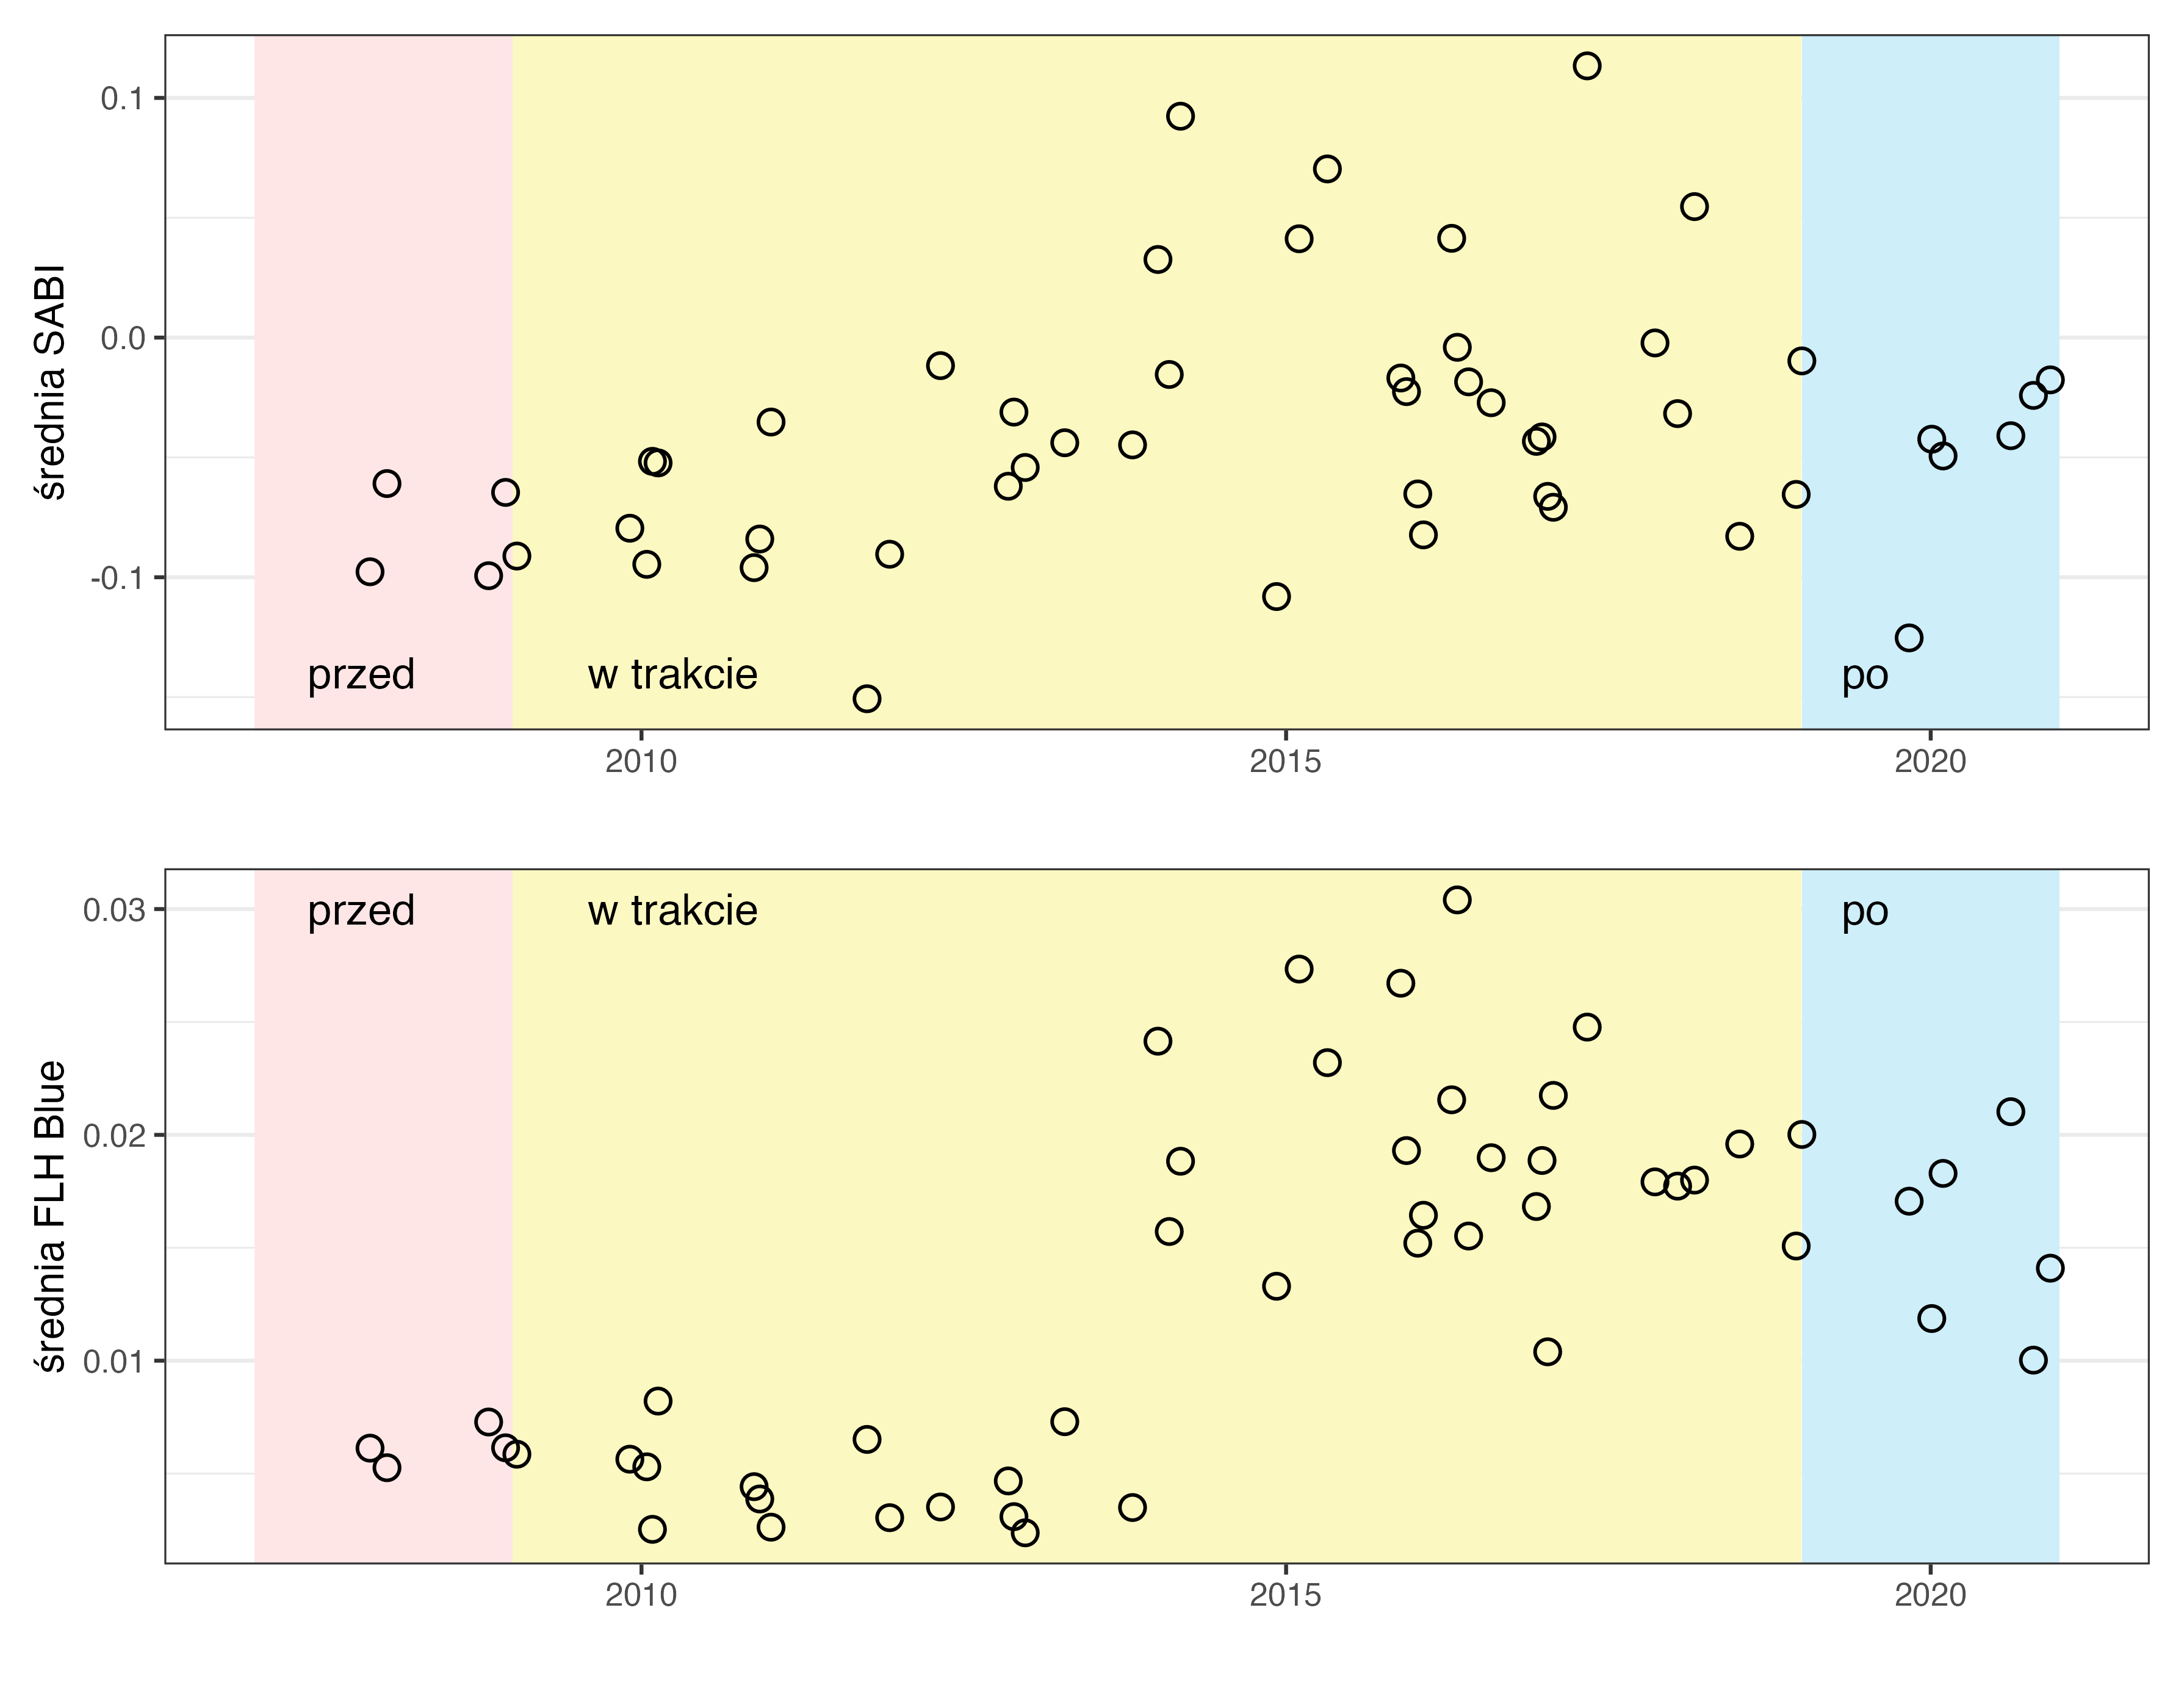
\includegraphics[width=6.25in,height=\textheight]{figures/nigeria/sabi_flhblue_means.png}

}

\caption{\label{fig-ng_sabi_flhblue_means}Rozkład średnich wartości
stężenia chlorofilu a dla Lagos. Każda kropka reprezentuje pojedynczy
obraz satelitarny, dla którego obliczono wskaźniki. Obserwacje
podzielono ze względu na etap prowadzonych prac: przed, w trakcie i po
zakończeniu. Czarna linia jest wygładzoną linią trendów.}

\end{figure}

Rycina~\ref{fig-ng_sabi_flhblue_means} przedstawia zmiany średnich
wartości wskaźników badających występowanie chlorofilu a wraz z upływem
czasu. Wskaźniki różnią się dynamiką zmian stężenia chlorofilu a w
Lagos. Wskaźnik SABI odnotował stały wzrost stężenia chlorofilu a od
początku rozpoczęcia prac do 2016 roku. Po tym roku, ilość chlorofilu a
w wodzie nieznacznie zmalała do poziomu, który utrzymał się po
zakończeniu prac. Wskaźnik FLH Blue przedstawia bardziej gwałtowną
zmianę stężenia. Ilość chlorofilu a w zbiorniku wodnym była stale niska
od rozpoczęcia prac do połowy okresu trwania konstrukcji. Pod koniec
2013 roku stężenie chlorofilu a drastycznie wzrosło. Wzrost ten pokrywa
się z momentem zwiększenia intensywności prac, podczas których utworzono
większość lądu. Wysoki poziom chlorofilu a utrzymywał się do 2016 roku,
po którym zaczął stopniowo maleć również w etapie po zakończeniu prac.

\begin{figure}[t]

{\centering 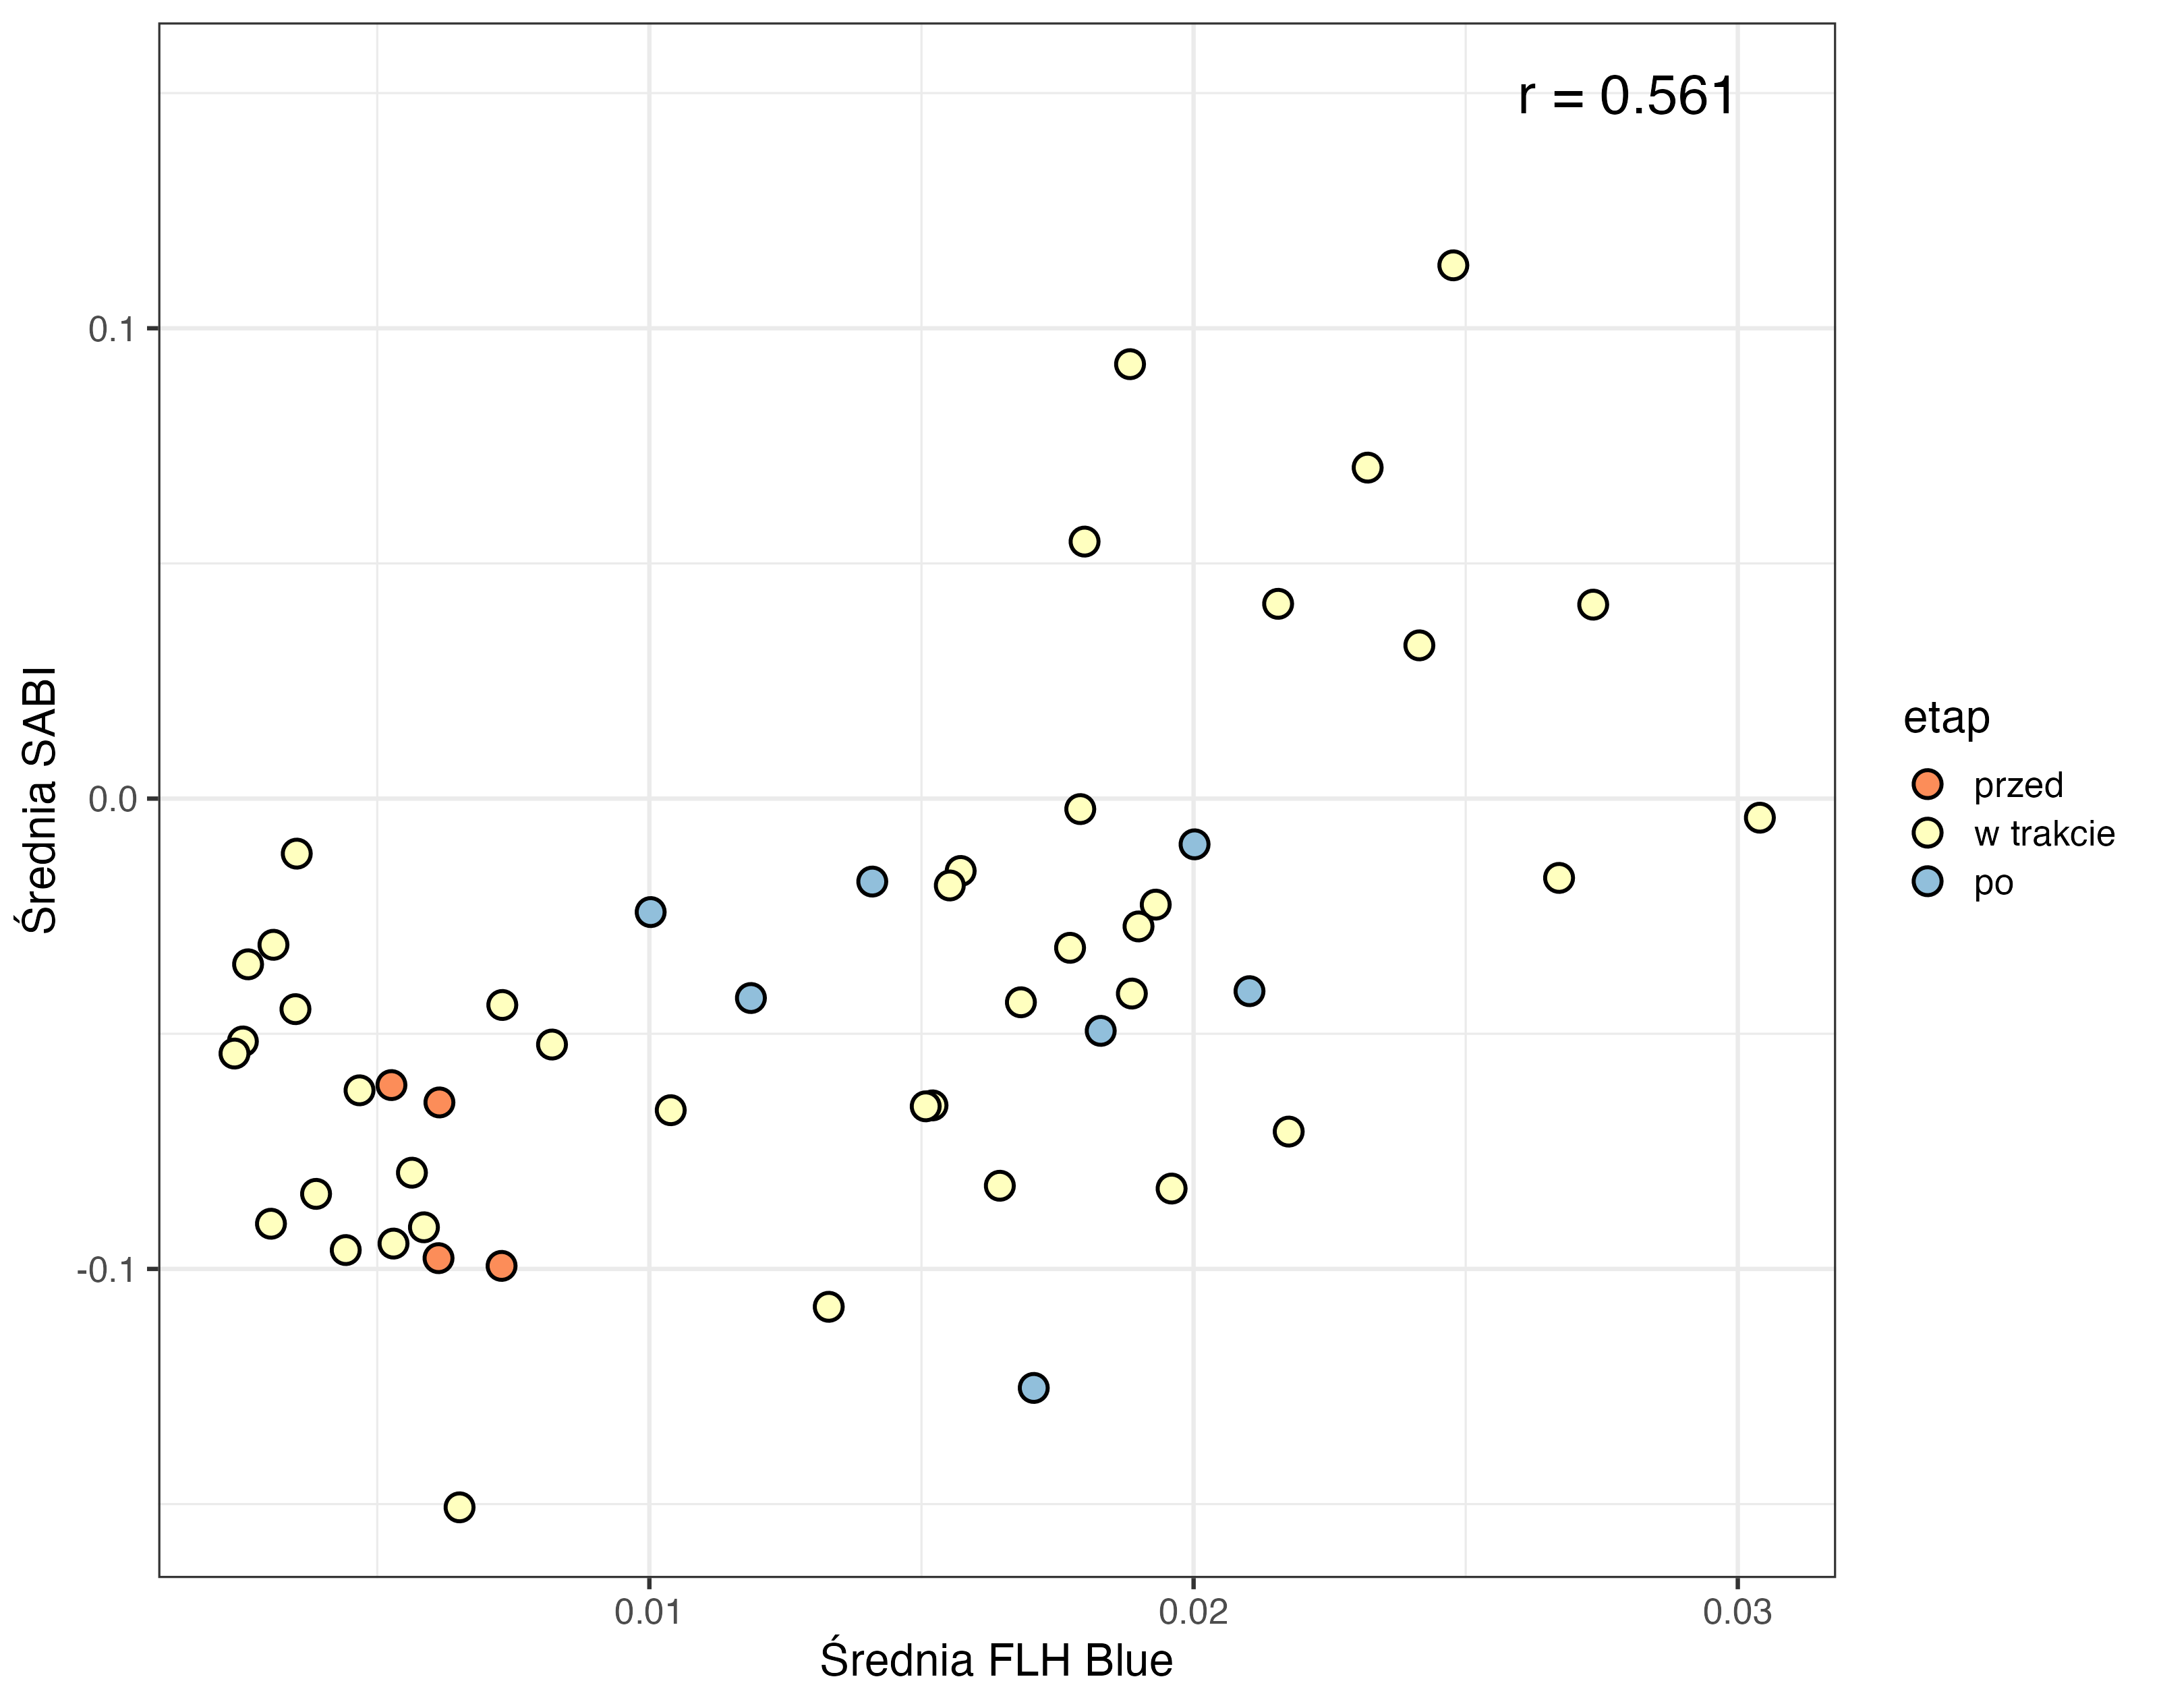
\includegraphics[width=4.16667in,height=\textheight]{figures/nigeria/sabi_flhblue_corr.png}

}

\caption{\label{fig-ng_sabi_flhblue_corr}Korelacja między średnimi
wartościami wskaźników SABI i FLH Blue dla Lagos. Każda kropka
reprezentuje pojedynczy obraz satelitarny, dla którego obliczono
wskaźniki. Obserwacje podzielono ze względu na etap prowadzonych prac:
przed, w trakcie i po zakończeniu.}

\end{figure}

Same średnie wartości dla obydwu wskaźników chlorofilu a wykazały
dodatnią korelację (Rycina~\ref{fig-ng_sabi_flhblue_corr}). Wraz ze
wzrostem stężenia chlorofilu a według wskaźnika SABI, wzrastało stężenie
chlorofilu a obliczonego przez wskaźnik FLH Blue. Oznacza to, że obydwa
wskaźniki są spójne w ocenie stężenia chlorofilu a dla obszaru badań w
Lagos.

\begin{figure}[t]

{\centering 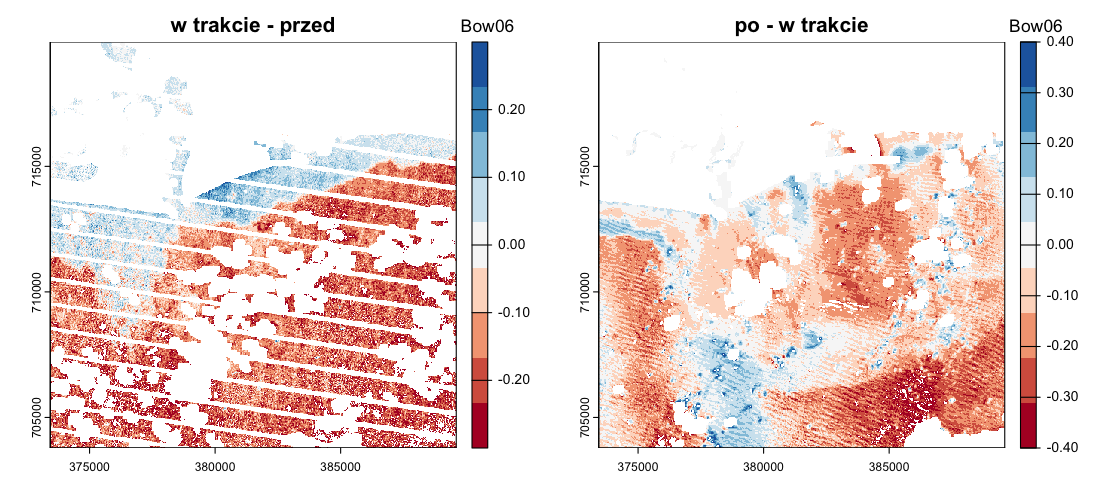
\includegraphics[width=6.25in,height=\textheight]{figures/nigeria/bow_diff.png}

}

\caption{\label{fig-ng_bow_diff}Mapy różnic występowania zawiesiny dla
Lagos, z wykorzystaniem wskaźnika Bow06. Rycina po lewej przedstawia
różnice między wskaźnikami, obliczonymi w trakcie trwania i przed
rozpoczęciem prac (grudzień 2015 i 2008). Rycina po prawej przedstawia
różnice między wskaźnikami, obliczonymi po zakończeniu prac i w trakcie
ich trwania (sierpień 2020 i 2016).}

\end{figure}

Rycina~\ref{fig-ng_bow_diff} przedstawia zmiany w rozkładzie
przestrzennym zawiesiny w wodzie w Lagos. Lewa rycina przedstawia, w
jaki sposób zmieniła się mętność wody podczas prowadzenia prac w
porównaniu do etapu przed rozpoczęciem prac. Dodatnie wartości znajdują
się na północy obszaru, czyli przy wybrzeżu i miejscu konstrukcji nowego
lądu. Oznacza to, że w wyniku prowadzenia prac nad stworzeniem nowego
lądu, mętność wody wzrosła przy wybrzeżu, co jest równoznaczne z
obniżeniem jakości wód dla tego obszaru. W wodach położonych dalej od
wybrzeża, stężenie zawiesiny było niższe niż przed rozpoczęciem pracy.
Prawa rycina zestawia stężenie zawiesiny po zakończeniu prac z okresem
ich prowadzenia. Dla obszaru badań w Lagos przeważają ujemne wartości,
co oznacza zmniejszenie mętności wody po skończeniu konstrukcji lądu.

Zmiany stężenia chlorofilu a w Lagos były znacznie większe, w porównaniu
do zmian w Dubaju. Najwyższe stężenia chlorofilu a zostały odnotowane w
trakcie prowadzenia prac konstrukcyjnych. Nie wykazano jednak istotności
statystycznej zmian wartości wskaźników między etapami prac. Stężenie
zawiesiny w wodzie w trakcie budowy lądu było mniejsze niż przed
rozpoczęciem prac, i stale malało po zakończeniu prac. Podczas trwania
prac, największa degradacja wody w postaci zwiększenia mętności miała
miejsce tuż przy wybrzeżu, w pobliżu konstrukcji nowego lądu. Pozostały
obszar był jednak niedotknięty pogorszeniem stanu wód. Raport
\textcite{EkoAtlantic2012}, odnośnie konstrukcji Eko Atlantic,
uwzględnił możliwość degradacji jakości wód, między innymi w wyniku
zwiększenia stężenia zawiesiny. W ramach pracy zaobserwowano jednak
odwrotną właściwość, gdzie po rozpoczęciu prac stężenie zawiesiny w
wodzie zmalało.

\hypertarget{limon-kostaryka-1}{%
\section{Limon, Kostaryka}\label{limon-kostaryka-1}}

\hypertarget{tbl-cr_stats}{}
\begin{table}
\caption{\label{tbl-cr_stats}Średnie wartości wskaźników jakości wody dla Limon, z podziałem na dwie
grupy parametrów jakości wód (chlorofil a i zawiesina) oraz na trzy
etapy prac (przed, w trakcie i po zakończeniu). W tabeli zawarto również
p-value z testu Kruskala-Wallisa, sprawdzającego istotność statystyczną
zmian średnich wartości wskaźników między etapami prac. }\tabularnewline

\centering
\begin{tabular}{lrrrr}
\toprule
  & przed (2014-2015) & w trakcie (2016-2018) & po (2019-2020) & p-value\\
\midrule
\addlinespace[0.3em]
\multicolumn{5}{l}{\textbf{chlorofil a}}\\
\hspace{1em}SABI & -0.002 & -0.021 & 0.001 & 0.858\\
\hspace{1em}FLH Blue & 0.013 & 0.012 & 0.011 & 0.539\\
\addlinespace[0.3em]
\multicolumn{5}{l}{\textbf{zawiesina}}\\
\hspace{1em}Bow06 & -0.134 & -0.103 & -0.120 & 0.542\\
\hspace{1em}Chip09 & -0.141 & -0.110 & -0.103 & 0.637\\
\bottomrule
\end{tabular}
\end{table}

Tabela~\ref{tbl-cr_stats} zawiera informacje o średnich wartościach
parametrów jakości wód dla Limon. Stężenie chlorofilu a po rozpoczęciu
prac zmniejszyło się. Po zakończeniu prac, wskaźnik SABI wykazał wzrost
chlorofilu a do najwyższych wartości spośród wszystkich etapów. Wskaźnik
FLH Blue od rozpoczęcia prac odnotował ciągły spadek stężenia chlorofilu
a w wodzie. W przypadku mętności wody, rozpoczęcie prac nad nowym lądem
zwiększyło stężenie zawiesiny w wodzie. Według wskaźnika Bow06, po
zakończeniu prac mętność wody ponownie zmniejszyła się. Chip09 wykazuje
natomiast dalszą degradację jakości wód.

\begin{figure}[t]

{\centering 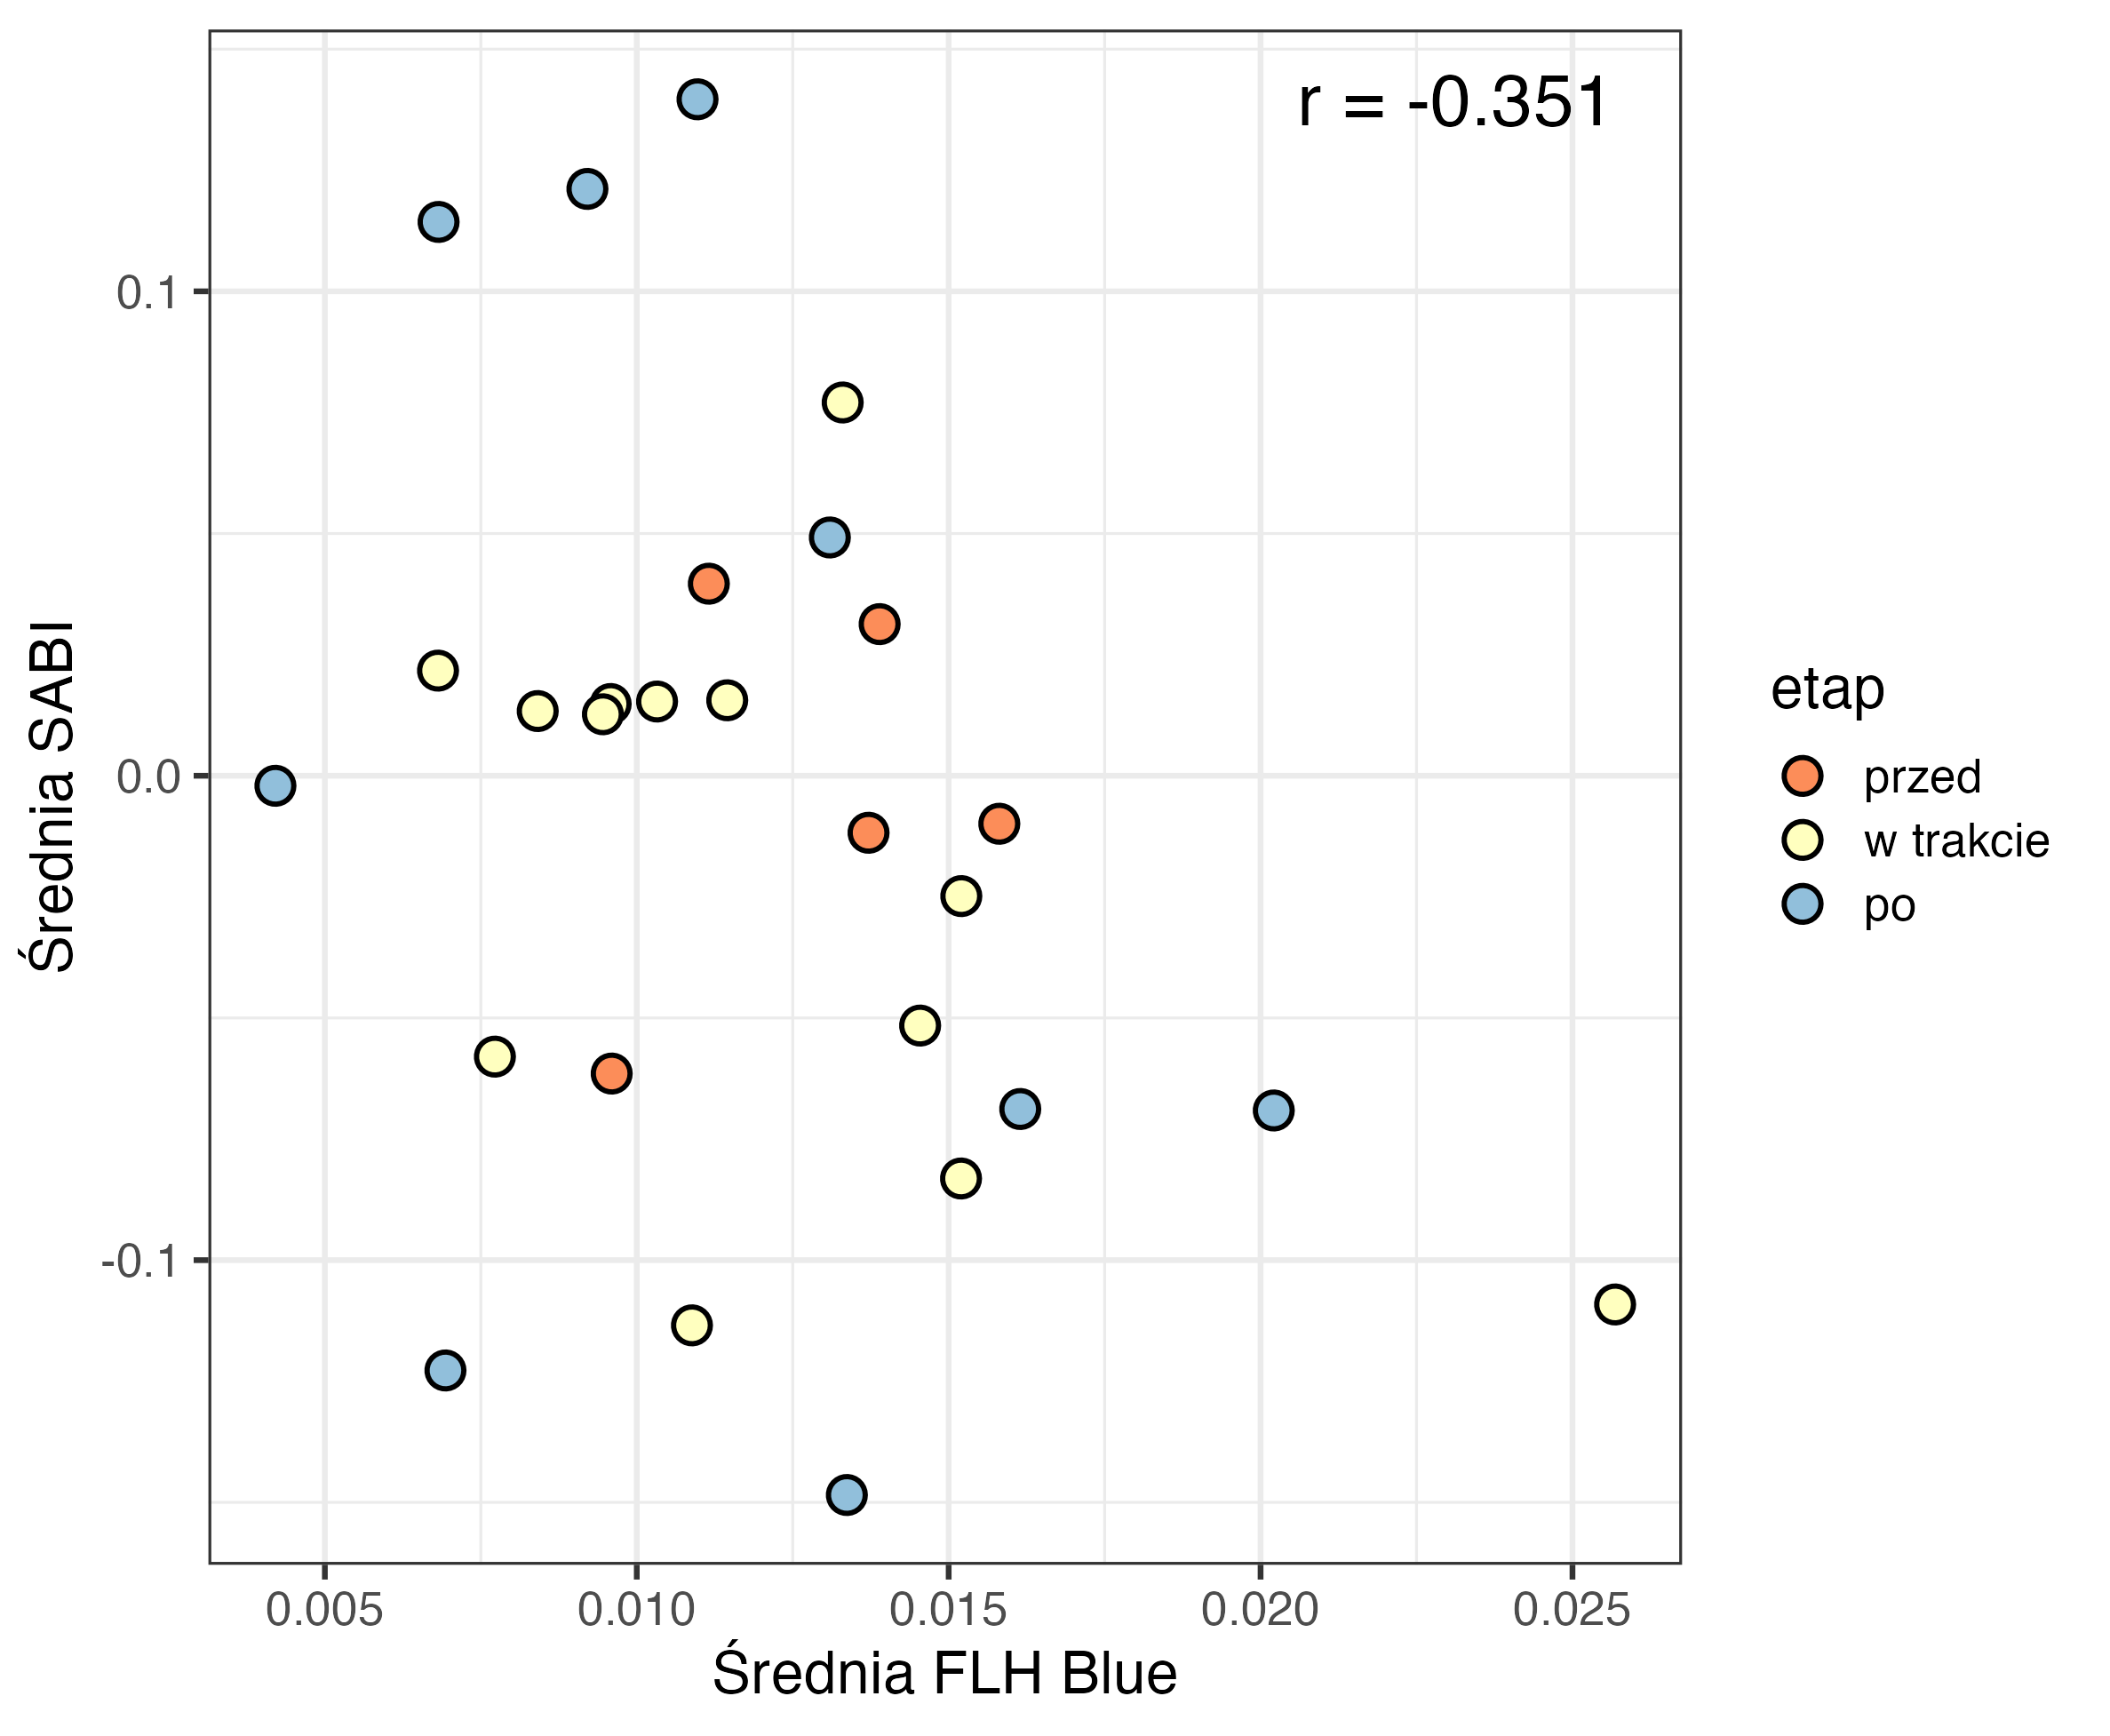
\includegraphics[width=4.16667in,height=\textheight]{figures/costarica/sabi_flhblue_corr.png}

}

\caption{\label{fig-cr_sabi_flhblue_corr}Korelacja między średnimi
wartościami wskaźników badających stężenie chlorofilu a dla Limon. Każda
kropka reprezentuje pojedynczy obraz satelitarny, dla którego obliczono
wskaźniki. Obserwacje podzielono ze względu na etap prowadzonych prac:
przed, w trakcie i po zakończeniu.}

\end{figure}

Rycina~\ref{fig-cr_sabi_flhblue_corr} przedstawia korelację między
wartościami wskaźników badających stężenia chlorofilu a. W
przeciwieństwie do korelacji wskaźników chlorofilu a w Lagos, w Limon
odnotowano ujemną korelację. Jest ona równocześnie słabsza. Wykazuje ona
zależność, według której wraz ze wzrostem odnotowanego stężenia
chlorofilu a przez wskaźnik SABI, maleje stężenie chlorofilu a według
wskaźnika FLH Blue. Tabela~\ref{tbl-cr_stats} pokazuje zależność, gdzie
obydwa wskaźniki wykazują przeciwne trendy zmian stężenia chlorofilu a.
Różnica w zmianach między dwoma wskaźnikami może wynikać z formuł obydwu
wskaźników. Wskaźnik SABI jest stosunkiem między kanałami barw
widzialnych i bliskiej podczerwieni. Wzór wskaźnika FLH Blue jest
natomiast różnicą między kanałami widzialnymi. Wykorzystanie kanału
bliskiej podczerwieni SABI mogło mieć wpływ na różnice w zmianach
wartości chlorofilu a według tego wskaźnika, a zmianami wskaźnika FLH
Blue.

\begin{figure}[t]

{\centering 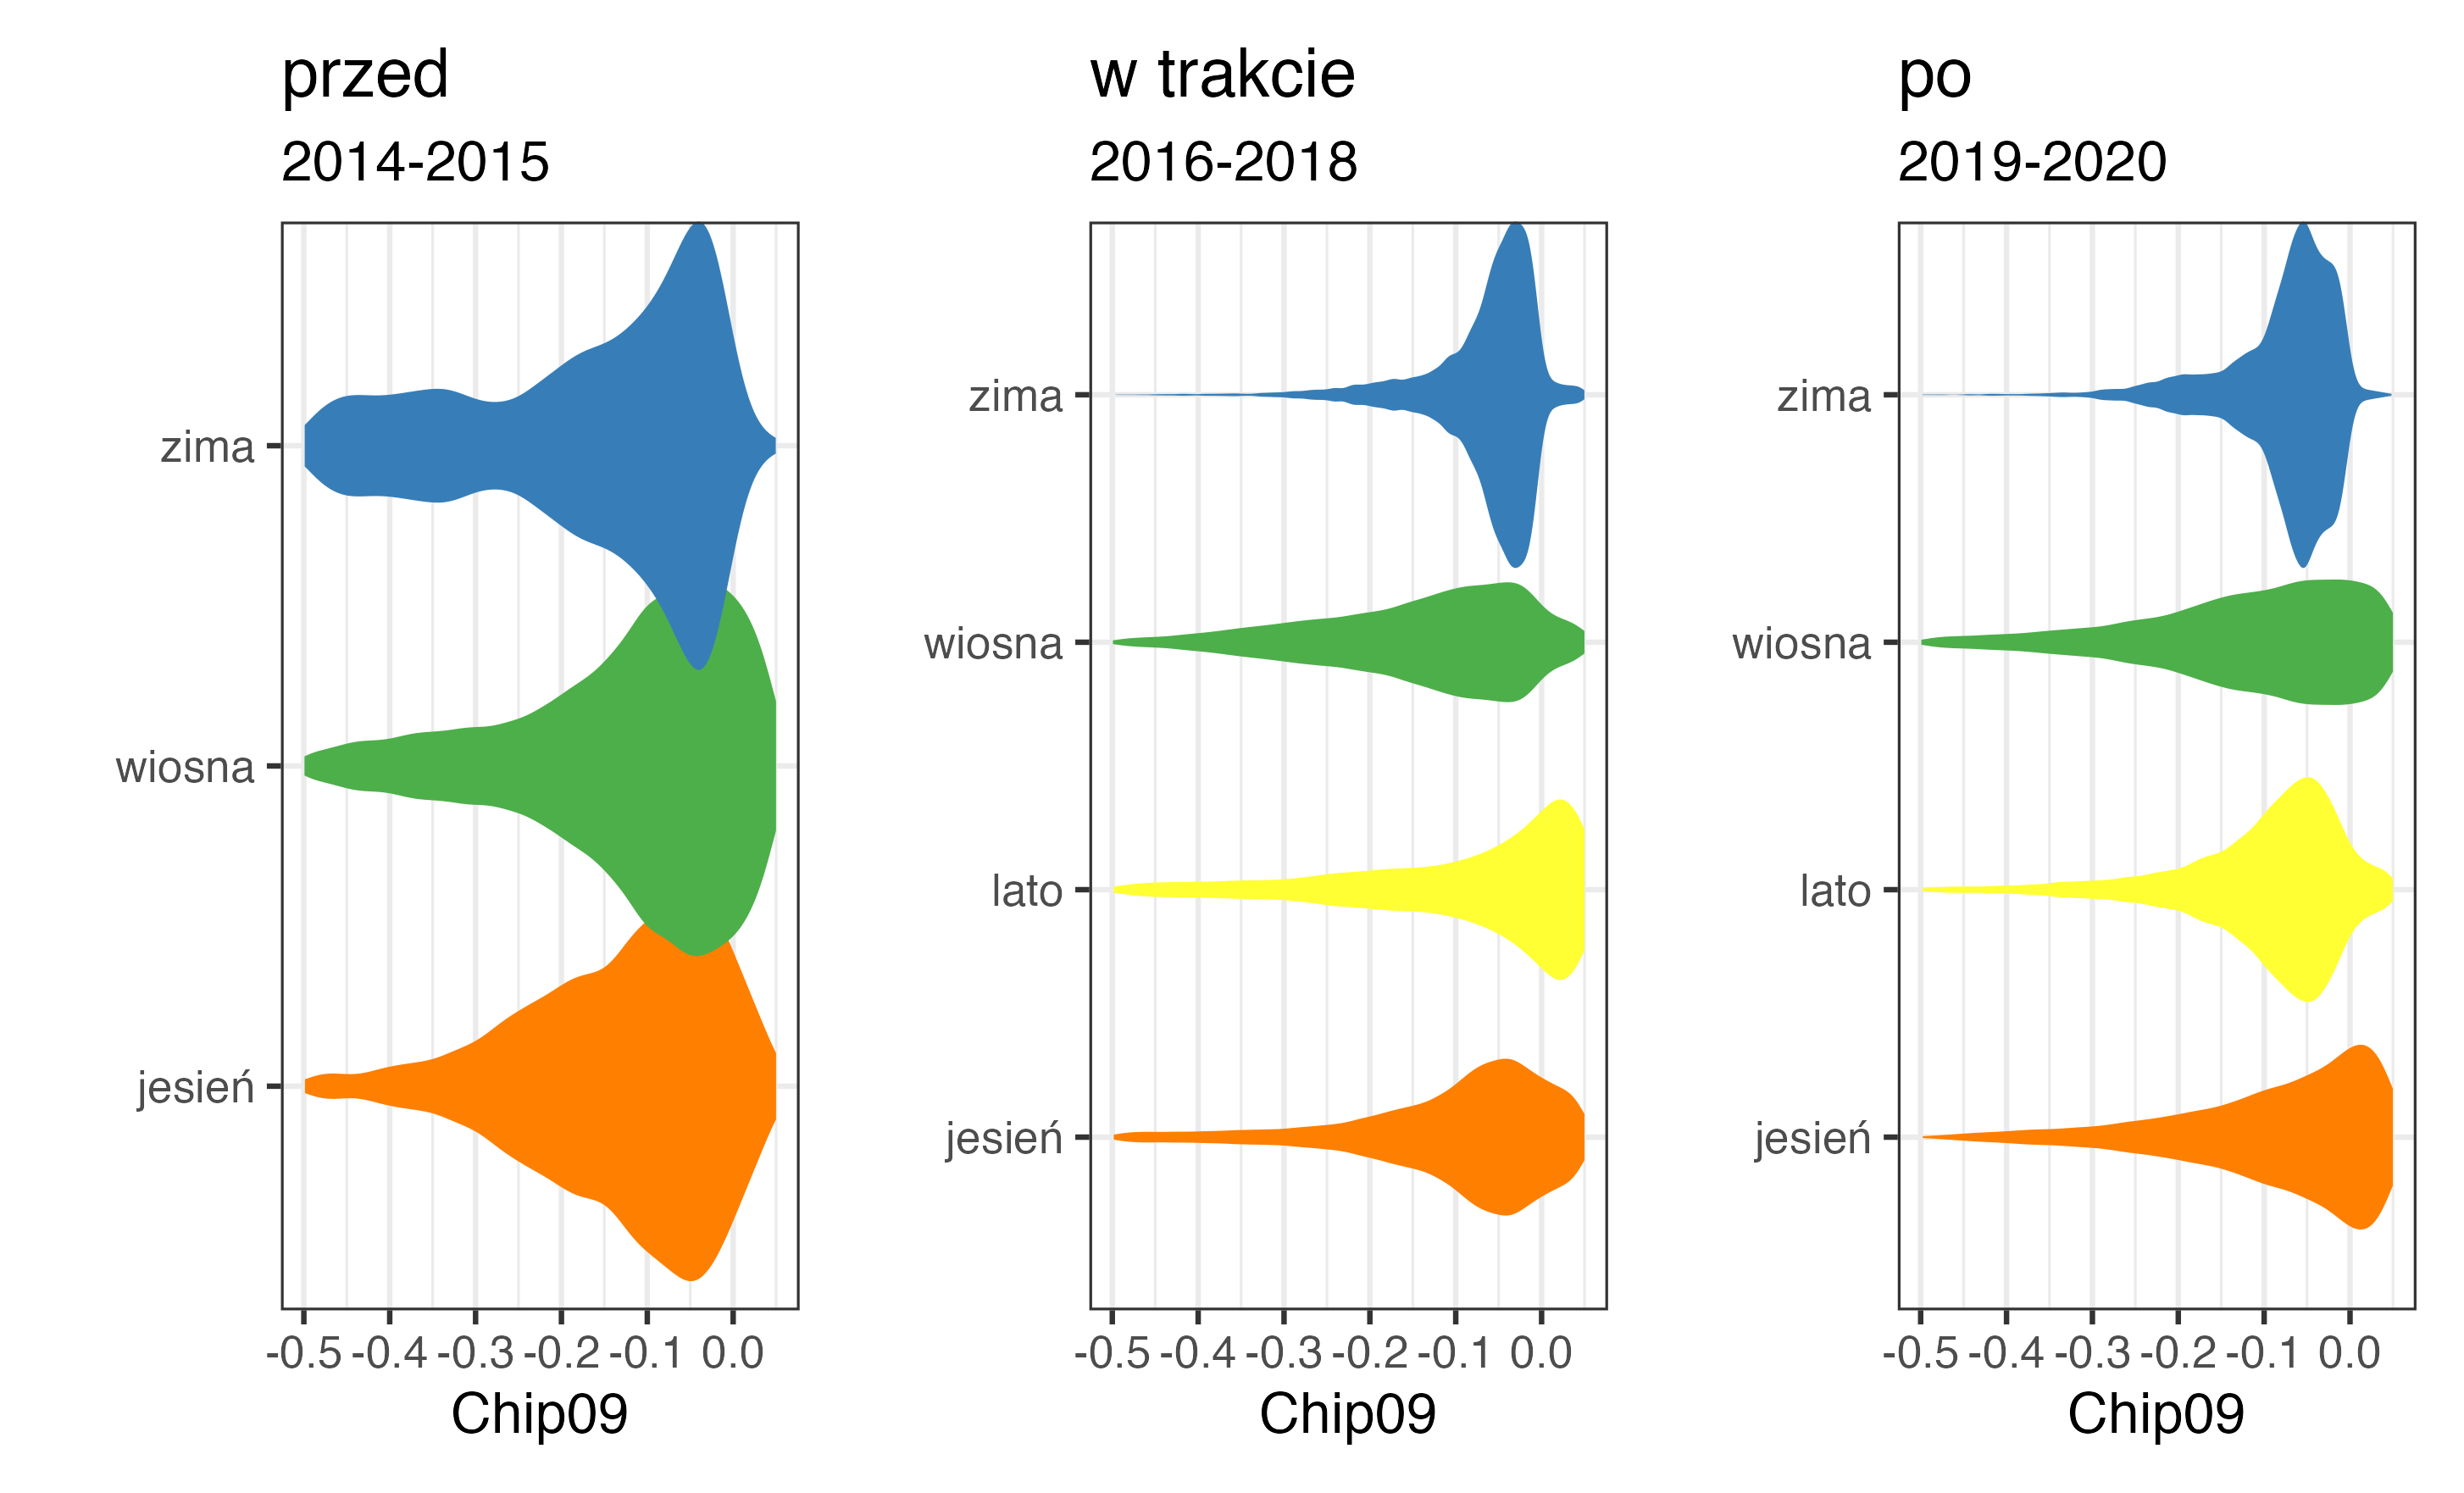
\includegraphics[width=6.25in,height=\textheight]{figures/costarica/chip_violin.png}

}

\caption{\label{fig-cr_chip_violin}Rozkład wartości stężenia zawiesiny
dla Limon na przykładzie wskaźnika Chip09, z podziałem na trzy etapy
prac: przed rozpoczęciem, w trakcie i po zakończeniu prac, oraz na
cztery pory roku.}

\end{figure}

Rycina~\ref{fig-cr_chip_violin} obrazuje różnice w rozkładach stężenia
zawiesiny, w zależności od etapu prac i pory roku. Wartości z etapu
trwania konstrukcji lądu cechują się większą jednorodnością, w
porównaniu do rozkładu wartości z etapu przed rozpoczęciem prac.
Większość wartości stężenia zawiesiny podczas trwania prac skupiona była
wokół najwyższych wartości. Oznacza to, że konstrukcja nowych lądów
zmniejszyła różnorodność stężenia zawiesiny na obszarze badań w Limon,
grupując wartości wokół średniej, wyższej niż przed rozpoczęciem prac.
Rozkład wartości po zakończeniu prac jest podobny do tego z okresu
trwania prac. Można wnioskować, że konstrukcja lądów zaburzyła rozkład
stężenia zawiesiny w skali badanego zakresu czasowego, ograniczając
stężenia zawiesiny do wartości zbliżonych do średniej.

\begin{figure}[t]

{\centering 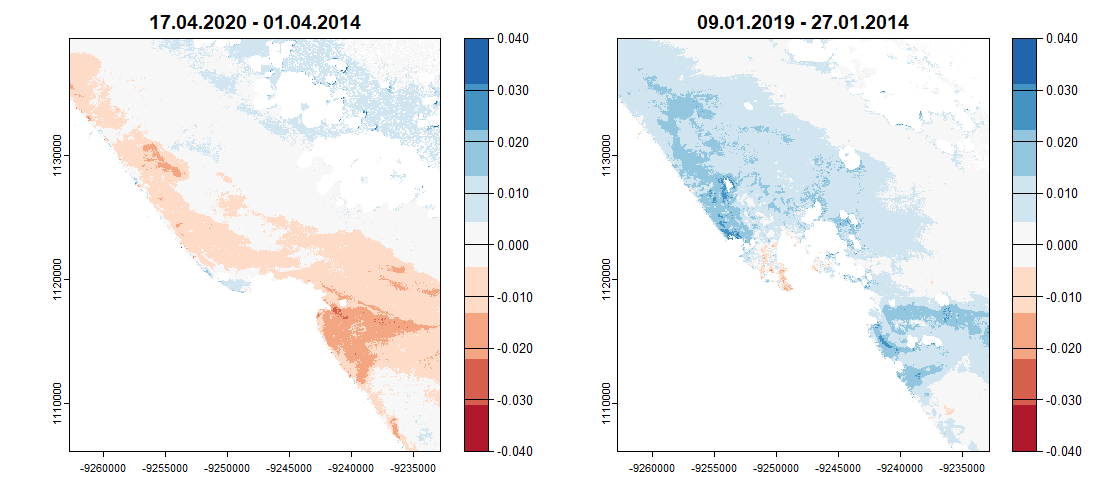
\includegraphics[width=6.25in,height=\textheight]{figures/costarica/flhblue_diff.png}

}

\caption{\label{fig-cr_flhblue_diff}Mapy różnic stężenia chlorofilu a
dla Limon, z wykorzystaniem wskaźnika FLH Blue. Rycina po lewej
przedstawia różnice między wskaźnikami, obliczonymi w trakcie trwania i
przed rozpoczęciem prac (maj 2018 i 2014). Rycina po prawej przedstawia
różnice między wskaźnikami, obliczonymi po zakończeniu prac i w trakcie
ich trwania (grudzień 2020 i 2016).}

\end{figure}

Rycina~\ref{fig-cr_flhblue_diff} przedstawia różnice w stężeniach
chlorofilu a dla poszczególnych etapów prac. Lewa rycina skupia się na
obserwacji zmian stężenia chlorofilu a w wodzie po rozpoczęciu prac, w
porównaniu do stanu przed. Wartości ujemne, tożsame ze spadkiem stężenia
chlorofilu a, dominują w pasie biegnącym od północnego zachodu do
południowego wschodu. Pokrywa się on z pasem wybrzeża Limon. Taki sam
trend zaobserwowano na prawej rycinie, porównującą stan wód po
zakończeniu prac. Ujemne wartości na tej rycinie wskazują, że stężenie
chlorofilu a było jeszcze mniejsze niż w trakcie konstrukcji lądów.
Zbiorniki wodne położone dalej od wybrzeża zanotowały wzrost stężenia
chlorofilu a.

Na obszarze badań w Limon odnotowano największą zmianę stężenia
chlorofilu a po rozpoczęciu prac konstrukcji nowego lądu. Jednocześnie,
testy wykazują najmniejszą istotność statystyczną spośród wszystkich
obszarów badań. Wynika to z liczby wykorzystanych danych, która dla
Limon była najmniejsza spośród wszystkich obszarów badań. Potwierdzenie
istotności zmian jakości wód między etapami prac wymaga pozyskania
większej liczby danych. W trakcie trwania prac, stężenie zawiesiny
również było największe. Zmiany obydwu parametrów sygnalizują o
znaczącym wpłynie konstrukcji nowych lądów na jakość wód w Limon.

\hypertarget{singapur-1}{%
\section{Singapur}\label{singapur-1}}

\hypertarget{tbl-sg_stats}{}
\begin{table}
\caption{\label{tbl-sg_stats}Średnie wartości wskaźników jakości wody dla Singapuru z podziałem na
dwie grupy parametrów jakości wód (chlorofil a i zawiesina) oraz na trzy
etapy prac (przed, w trakcie i po zakończeniu). W tabeli zawarto również
p-value z testu Kruskala-Wallisa, sprawdzającego istotność statystyczną
zmian średnich wartości wskaźników między etapami prac. }\tabularnewline

\centering
\begin{tabular}{lrrrr}
\toprule
  & przed (1991-1992) & w trakcie (1993-2003) & po (2004-2005) & p-value\\
\midrule
\addlinespace[0.3em]
\multicolumn{5}{l}{\textbf{chlorofil a}}\\
\hspace{1em}SABI & -0.070 & -0.098 & -0.089 & 0.309\\
\hspace{1em}FLH Blue & 0.021 & 0.020 & 0.016 & 0.053\\
\addlinespace[0.3em]
\multicolumn{5}{l}{\textbf{zawiesina}}\\
\hspace{1em}Bow06 & 0.553 & 0.532 & 0.475 & 0.202\\
\hspace{1em}Chip09 & 0.410 & 0.334 & 0.290 & 0.432\\
\bottomrule
\end{tabular}
\end{table}

Tabela~\ref{tbl-sg_stats} wskazuje na zmiany wartości parametrów jakości
wód w trakcie trwania prac tworzenia nowych lądów. Wskaźniki badające
wartości stężenia chlorofilu a wykryły spadek wartości w etapie
prowadzenia prac, porównując je do stanu przed rozpoczęciem prac.
Wskaźniki spektralne różnią się od siebie natomiast średnimi wartościami
chlorofilu a po zakończeniu prac. Według SABI, stężenie chlorofilu a
wzrośnie po zakończeniu konstrukcji nowych lądów. Wskaźnik FLH Blue
wskazuje natomiast na kontynuację zaniku chlorofilu a, rozpoczętą w
etapie prowadzenia prac. Stężenie zawiesiny w wodzie dla obszaru badań w
Singapurze uległo zmniejszeniu wraz z upływem lat. Dla obydwu
wskaźników, średnie wartości zawiesiny były najwyższe przed rozpoczęciem
prac, a najniższe -- po ich zakończeniu. Wskazuje to na potencjalny
wpływ konstrukcji nowych lądów na zmniejszenie mętności wody.

\begin{figure}[t]

{\centering 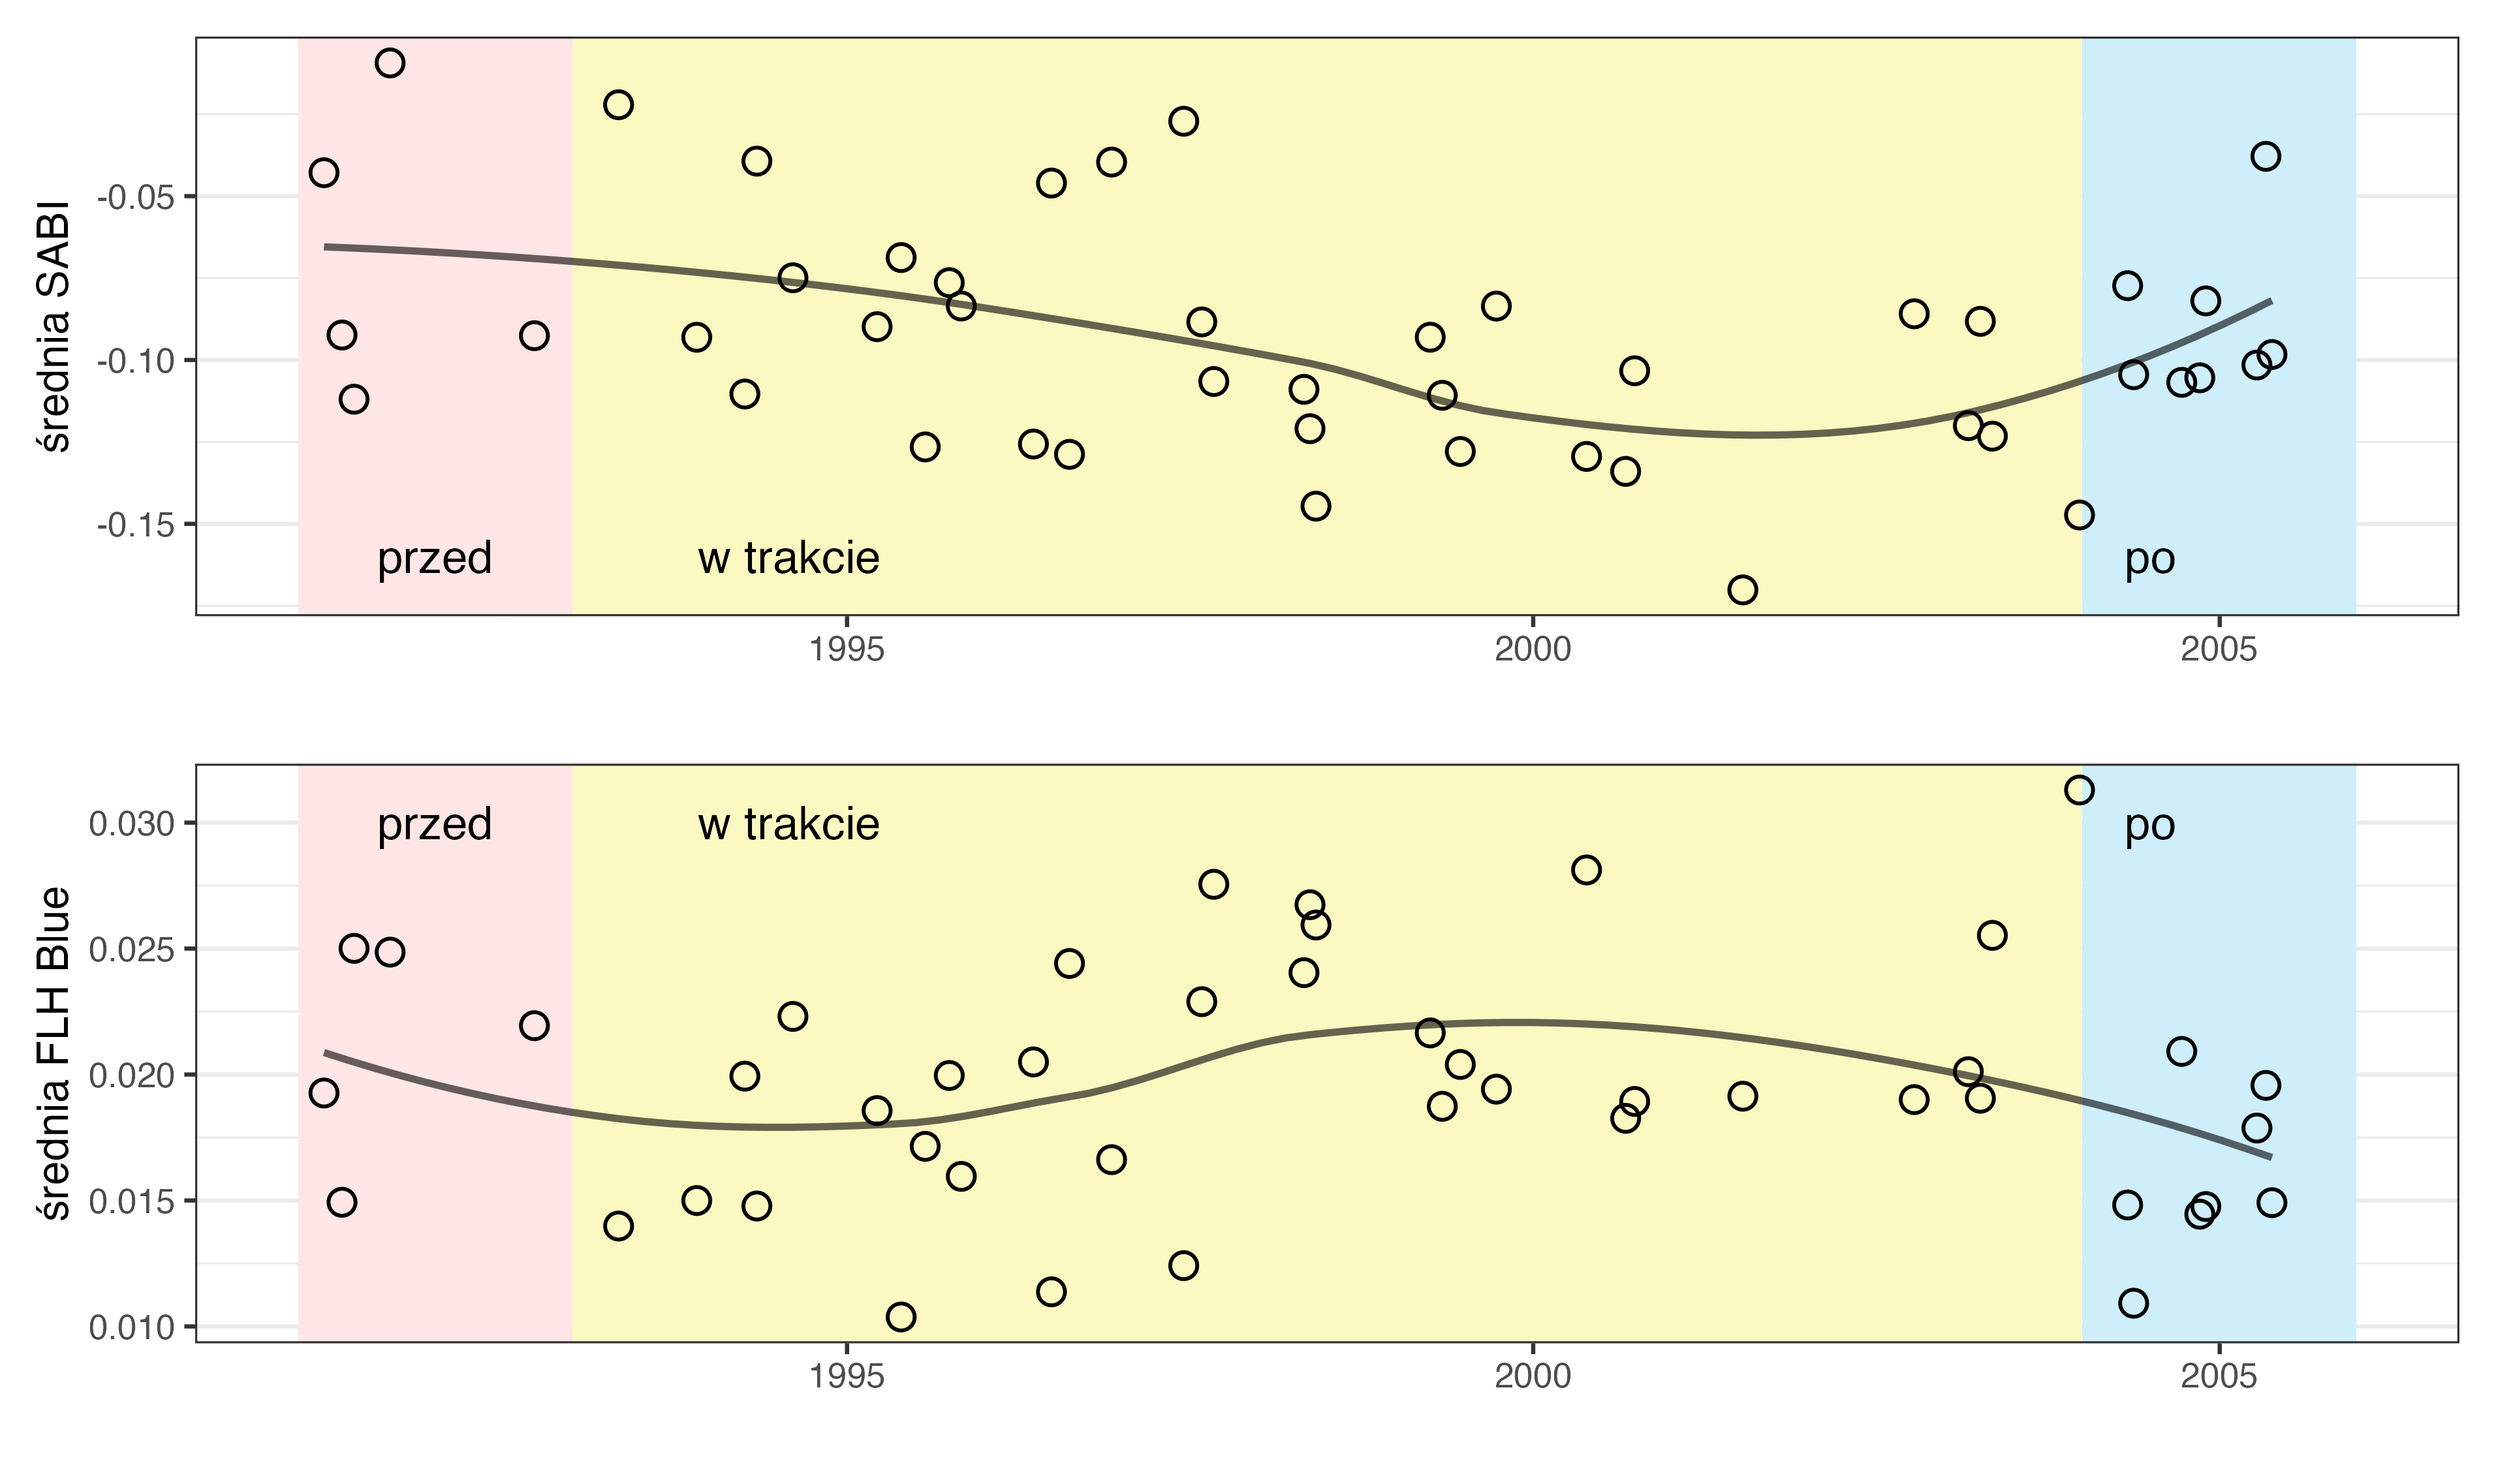
\includegraphics[width=6.25in,height=\textheight]{figures/singapore/sabi_flhblue_means.png}

}

\caption{\label{fig-sg_sabi_flhblue_means}Rozkład średnich wartości
stężenia chlorofilu a dla Singapuru. Każda kropka reprezentuje
pojedynczy obraz satelitarny, dla którego obliczono wskaźniki.
Obserwacje podzielono ze względu na etap prowadzonych prac: przed, w
trakcie i po zakończeniu. Czarna linia jest wygładzoną linią trendów.}

\end{figure}

Rycina~\ref{fig-sg_sabi_flhblue_means} przedstawia zmiany średnich
wartości stężeń chlorofilu a w Singapurze. Największe spadki średnich
wartości stężenia chlorofilu odnotowano podczas prowadzenia prac
konstrukcyjnych. Dodatkowo, widoczne są różnice między wskaźnikami w
zmianach średnich wartości w czasie. SABI przedstawia trend zmniejszania
sie stężenia chlorofilu a w wodzie przez większość okresu trwania prac.
Wskaźnik FLH Blue natomiast przez pierwszą połowę etapu konstrukcji lądu
odnotowywał wzrost stężenia chlorofilu a. W 1997 roku stężenie
chlorofilu a zaczęło maleć aż do momentu zakończenia prac, gdzie
osiągnęło najniższy poziom.

\begin{figure}[t]

{\centering 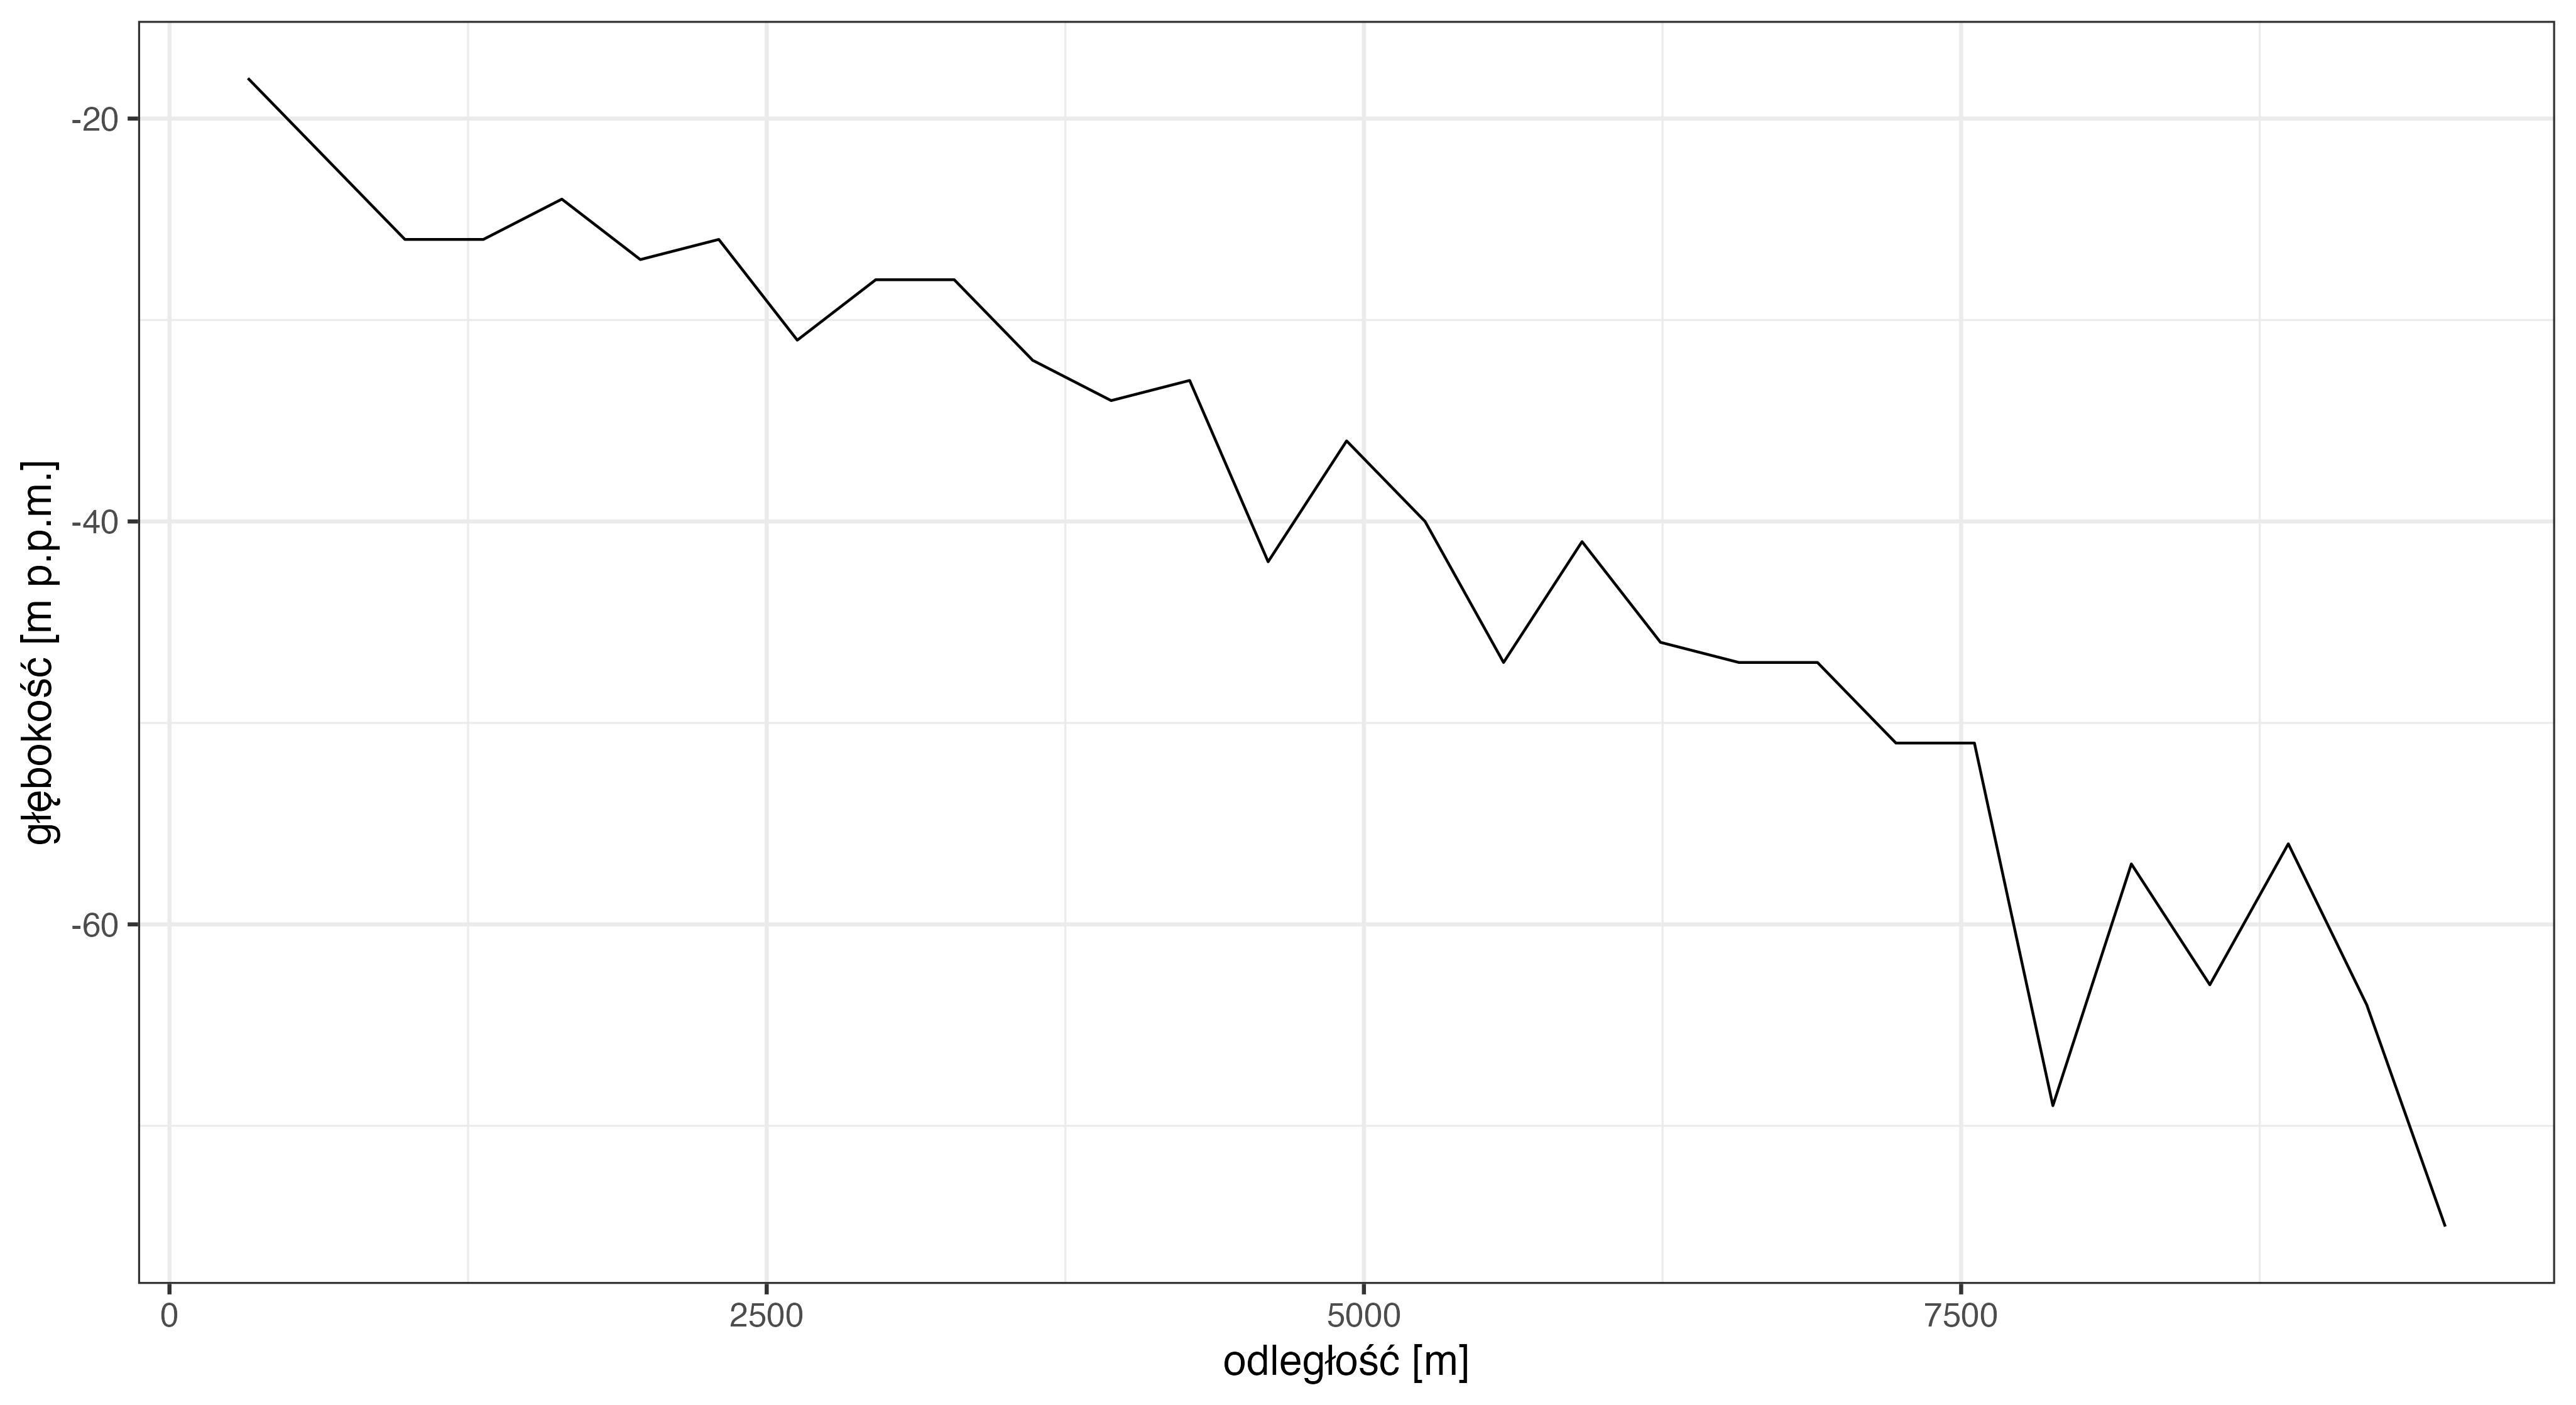
\includegraphics[width=3.64583in,height=\textheight]{figures/singapore/profile.png}

}

\caption{\label{fig-sg_profile}Zmiany głębokości zbiornika wodnego
wzdłuż profilu dla Singapuru.}

\end{figure}

\begin{figure}[t]

{\centering 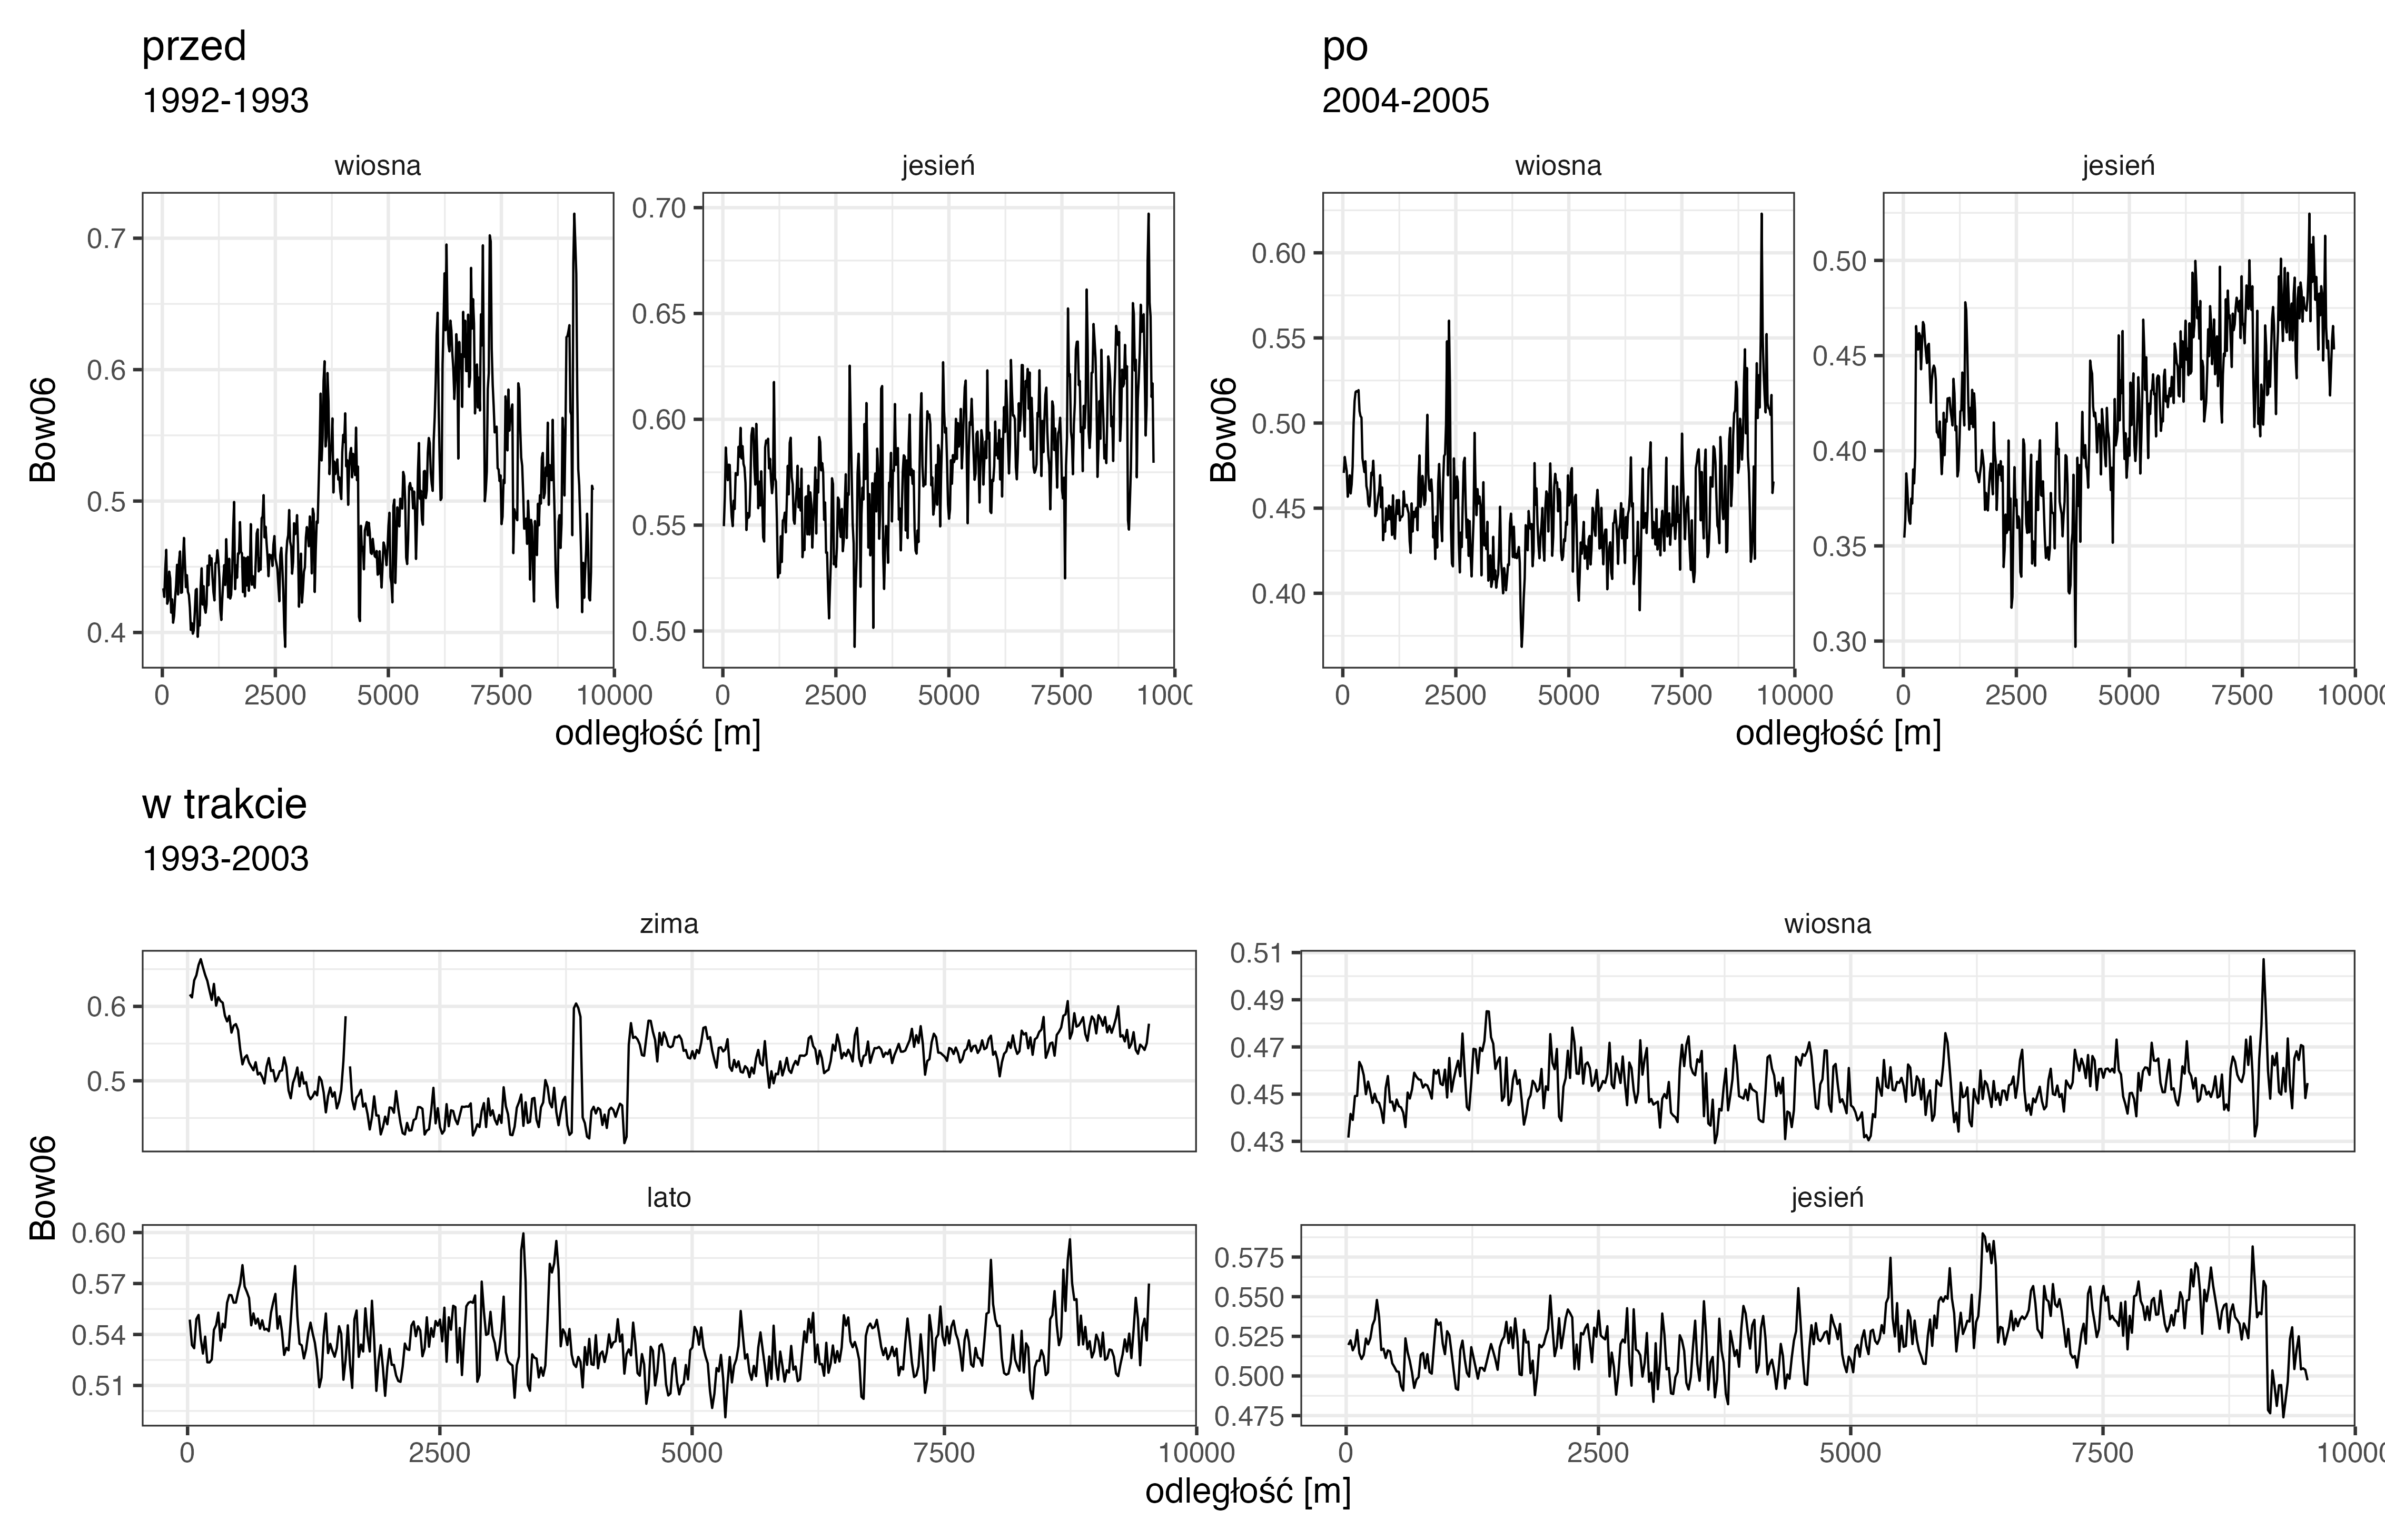
\includegraphics[width=6.77083in,height=\textheight]{figures/singapore/bow_profile.png}

}

\caption{\label{fig-sg_bow_profile}Zmiany wartości stężenia zawiesiny a
wzdłuż profilu dla Singapuru, na podstawie wskaźnika Bow06. Rycina
składa się z trzech paneli: zmiany wartości dla obrazów przed
rozpoczęciem prac, w trakcie trwania prac i po zakończeniu prac. Każdy z
paneli podzielony jest na poszczególne pory roku. Czerwona linia jest
wygładzoną linią trendów.}

\end{figure}

Rycina~\ref{fig-sg_bow_profile} przedstawia zmiany w stężeniu zawiesiny
w wodzie wzdłuż profilu. Rycina~\ref{fig-sg_profile} pokazuje, że
dynamika zmian wartości zawiesiny wraz z odległością pokrywa się ze
zmianą głębokości. Przy odległości 2500 metrów, dno zbiornika zaczyna
stawać się głębsze, schodząc od 25 do 70 metrów głębokości na końcu
profilu. Wpływ zmian głębokości na stężenie zawiesiny jest widoczny na
obserwacjach z przed i po zakończeniu prac. Wraz z oddalaniem się od
brzegu, stężenie zawiesiny zaczyna wzrastać. Trend ten natomiast nie
jest widoczny dla obserwacji z etapu przeprowadzania konstrukcji nowego
lądu. Zmiany stężenia zawiesiny w wodzie podczas trwania prac są
bardziej zróżnicowanie i nie wykazują powiązania ze zmianą głębokości
zbiornika wodnego. Wskazuje to na potencjalny wpływ tworzenia nowych
lądów na powstawanie zaburzeń w rozkładzie przestrzennym stężeń
zawiesiny.

\begin{figure}[t]

{\centering 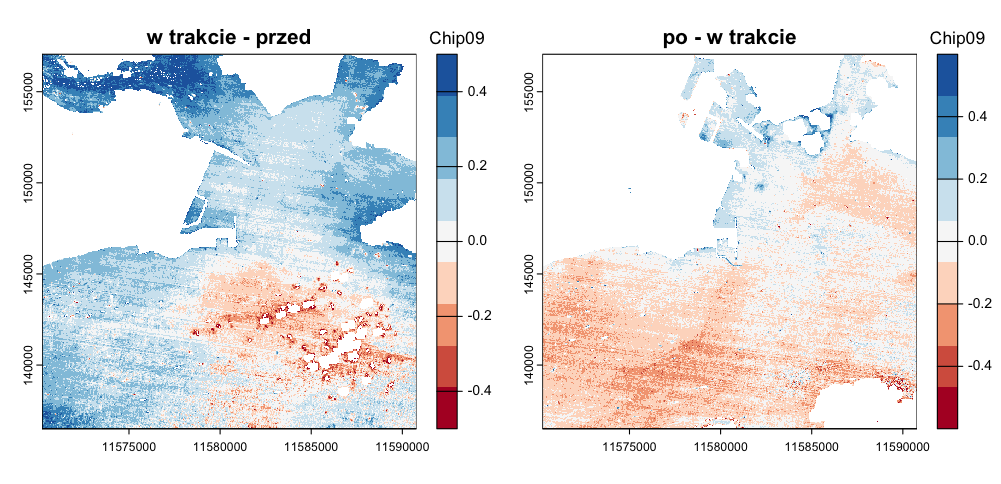
\includegraphics[width=6.25in,height=\textheight]{figures/singapore/chip_diff.png}

}

\caption{\label{fig-sg_chip_diff}Mapy różnic stężenia zawiesiny dla
Singapuru, z wykorzystaniem wskaźnika Chip09. Rycina po lewej
przedstawia różnice między wskaźnikami, obliczonymi w trakcie trwania i
przed rozpoczęciem prac (kwiecień 1999 i 1991). Rycina po prawej
przedstawia różnice między wskaźnikami, obliczonymi po zakończeniu prac
i w trakcie ich trwania (listopad 2004 i 1995).}

\end{figure}

Rycina~\ref{fig-sg_chip_diff} przedstawia różnice w stężeniu zawiesiny
między wybranymi etapami prac. Lewa rycina porównuje mętność wody w
trakcie prowadzenia prac ze stanem przed ich rozpoczęciem. Większości
obszaru przypisane zostały dodatnie wartości. Utożsamiane są one ze
wzrostem stężenia zawiesiny w wodzie. Oznacza to, że rozpoczęcie prac
tworzenia nowych lądów w Singapurze wpłynęło na zwiększenie mętności
wody na większości obszaru badań. Prawa rycina porównuje stężenie
zawiesiny w zbiorniku wodnym po zakończeniu prac, ze stanem wody w
trakcie prowadzenia prac. Na tej rycinie przeważają wartości ujemne,
oznaczające zmniejszenie mętności wody. Wzrost stężenia zawiesiny po
zakończeniu prac w Singapurze odnotowano jedynie na północnym obszarze,
na którym powstał nowy ląd.

Test Kruskala-Wallisa wskazał zmiany średnich wartości wskaźnika FLH
Blue między etapami prac jako istotne statystycznie. Wskaźnik ten
odnotował spadek stężenia chlorofilu a po rozpoczęciu konstrukcji lądu w
Singapurze. Wraz z rozpoczęciem konstrukcji nowych lądów, stężenie
zawiesiny również zmniejszało się. Najniższe wartości stężenia zawiesiny
zostały odnotowane po zakończeniu prac. Zmiany te można uznać jako
pozytywny sygnał poprawy jakości wód. Procesy tworzenia nowych lądów
miały jednak negatywny wpływ na rozkład przestrzenny stężenia zawiesiny.
Uległ on rozproszeniu, i w przeciwieństwie do pozostałych etapów prac,
podczas tworzenia nowych lądów nie wykryto zależności między zmianą
głębokości a zmianą stężenia zawiesiny.

\hypertarget{szanghaj-chiny-1}{%
\section{Szanghaj, Chiny}\label{szanghaj-chiny-1}}

\hypertarget{tbl-cn_stats}{}
\begin{table}
\caption{\label{tbl-cn_stats}Średnie wartości wskaźników jakości wody dla Szanghaju z podziałem na
dwie grupy parametrów jakości wód (chlorofil a i zawiesina) oraz na trzy
etapy prac (przed, w trakcie i po zakończeniu). W tabeli zawarto również
p-value z testu Kruskala-Wallisa, sprawdzającego istotność statystyczną
zmian średnich wartości wskaźników między etapami prac. }\tabularnewline

\centering
\begin{tabular}{lrrrr}
\toprule
  & przed (2000-2002) & w trakcie (2003-2005) & po (2006-2008) & p-value\\
\midrule
\addlinespace[0.3em]
\multicolumn{5}{l}{\textbf{chlorofil a}}\\
\hspace{1em}SABI & -0.313 & -0.289 & -0.281 & 0.178\\
\hspace{1em}FLH Blue & 0.015 & 0.018 & 0.023 & 0.028\\
\addlinespace[0.3em]
\multicolumn{5}{l}{\textbf{zawiesina}}\\
\hspace{1em}Bow06 & 0.965 & 0.972 & 0.967 & 0.985\\
\hspace{1em}Chip09 & 0.471 & 0.496 & 0.507 & 0.258\\
\bottomrule
\end{tabular}
\end{table}

Tabela~\ref{tbl-cn_stats} przedstawia zmiany średnich wartości stężeń
parametrów oceny jakości wód. Wraz z upływem lat, stężenie chlorofilu a
w zbiornikach wodnym na obszarze badań w Szanghaju stale wzrastało.
Trend ten jest widoczny na obydwu wskaźnikach. Podobne zmiany
zaobserwowano dla stężenia zawiesiny. Mętność wody wzrosła po
rozpoczęciu prac, i po ich zakończeniu ponownie wzrosła według wskaźnika
Chip09, lub spadła według wskaźnika Bow06. Stężenie chlorofilu a
cechowało się większymi zmianami wartości, w porównaniu do wartości
wskaźników opisujących mętność wody.

\begin{figure}[t]

{\centering 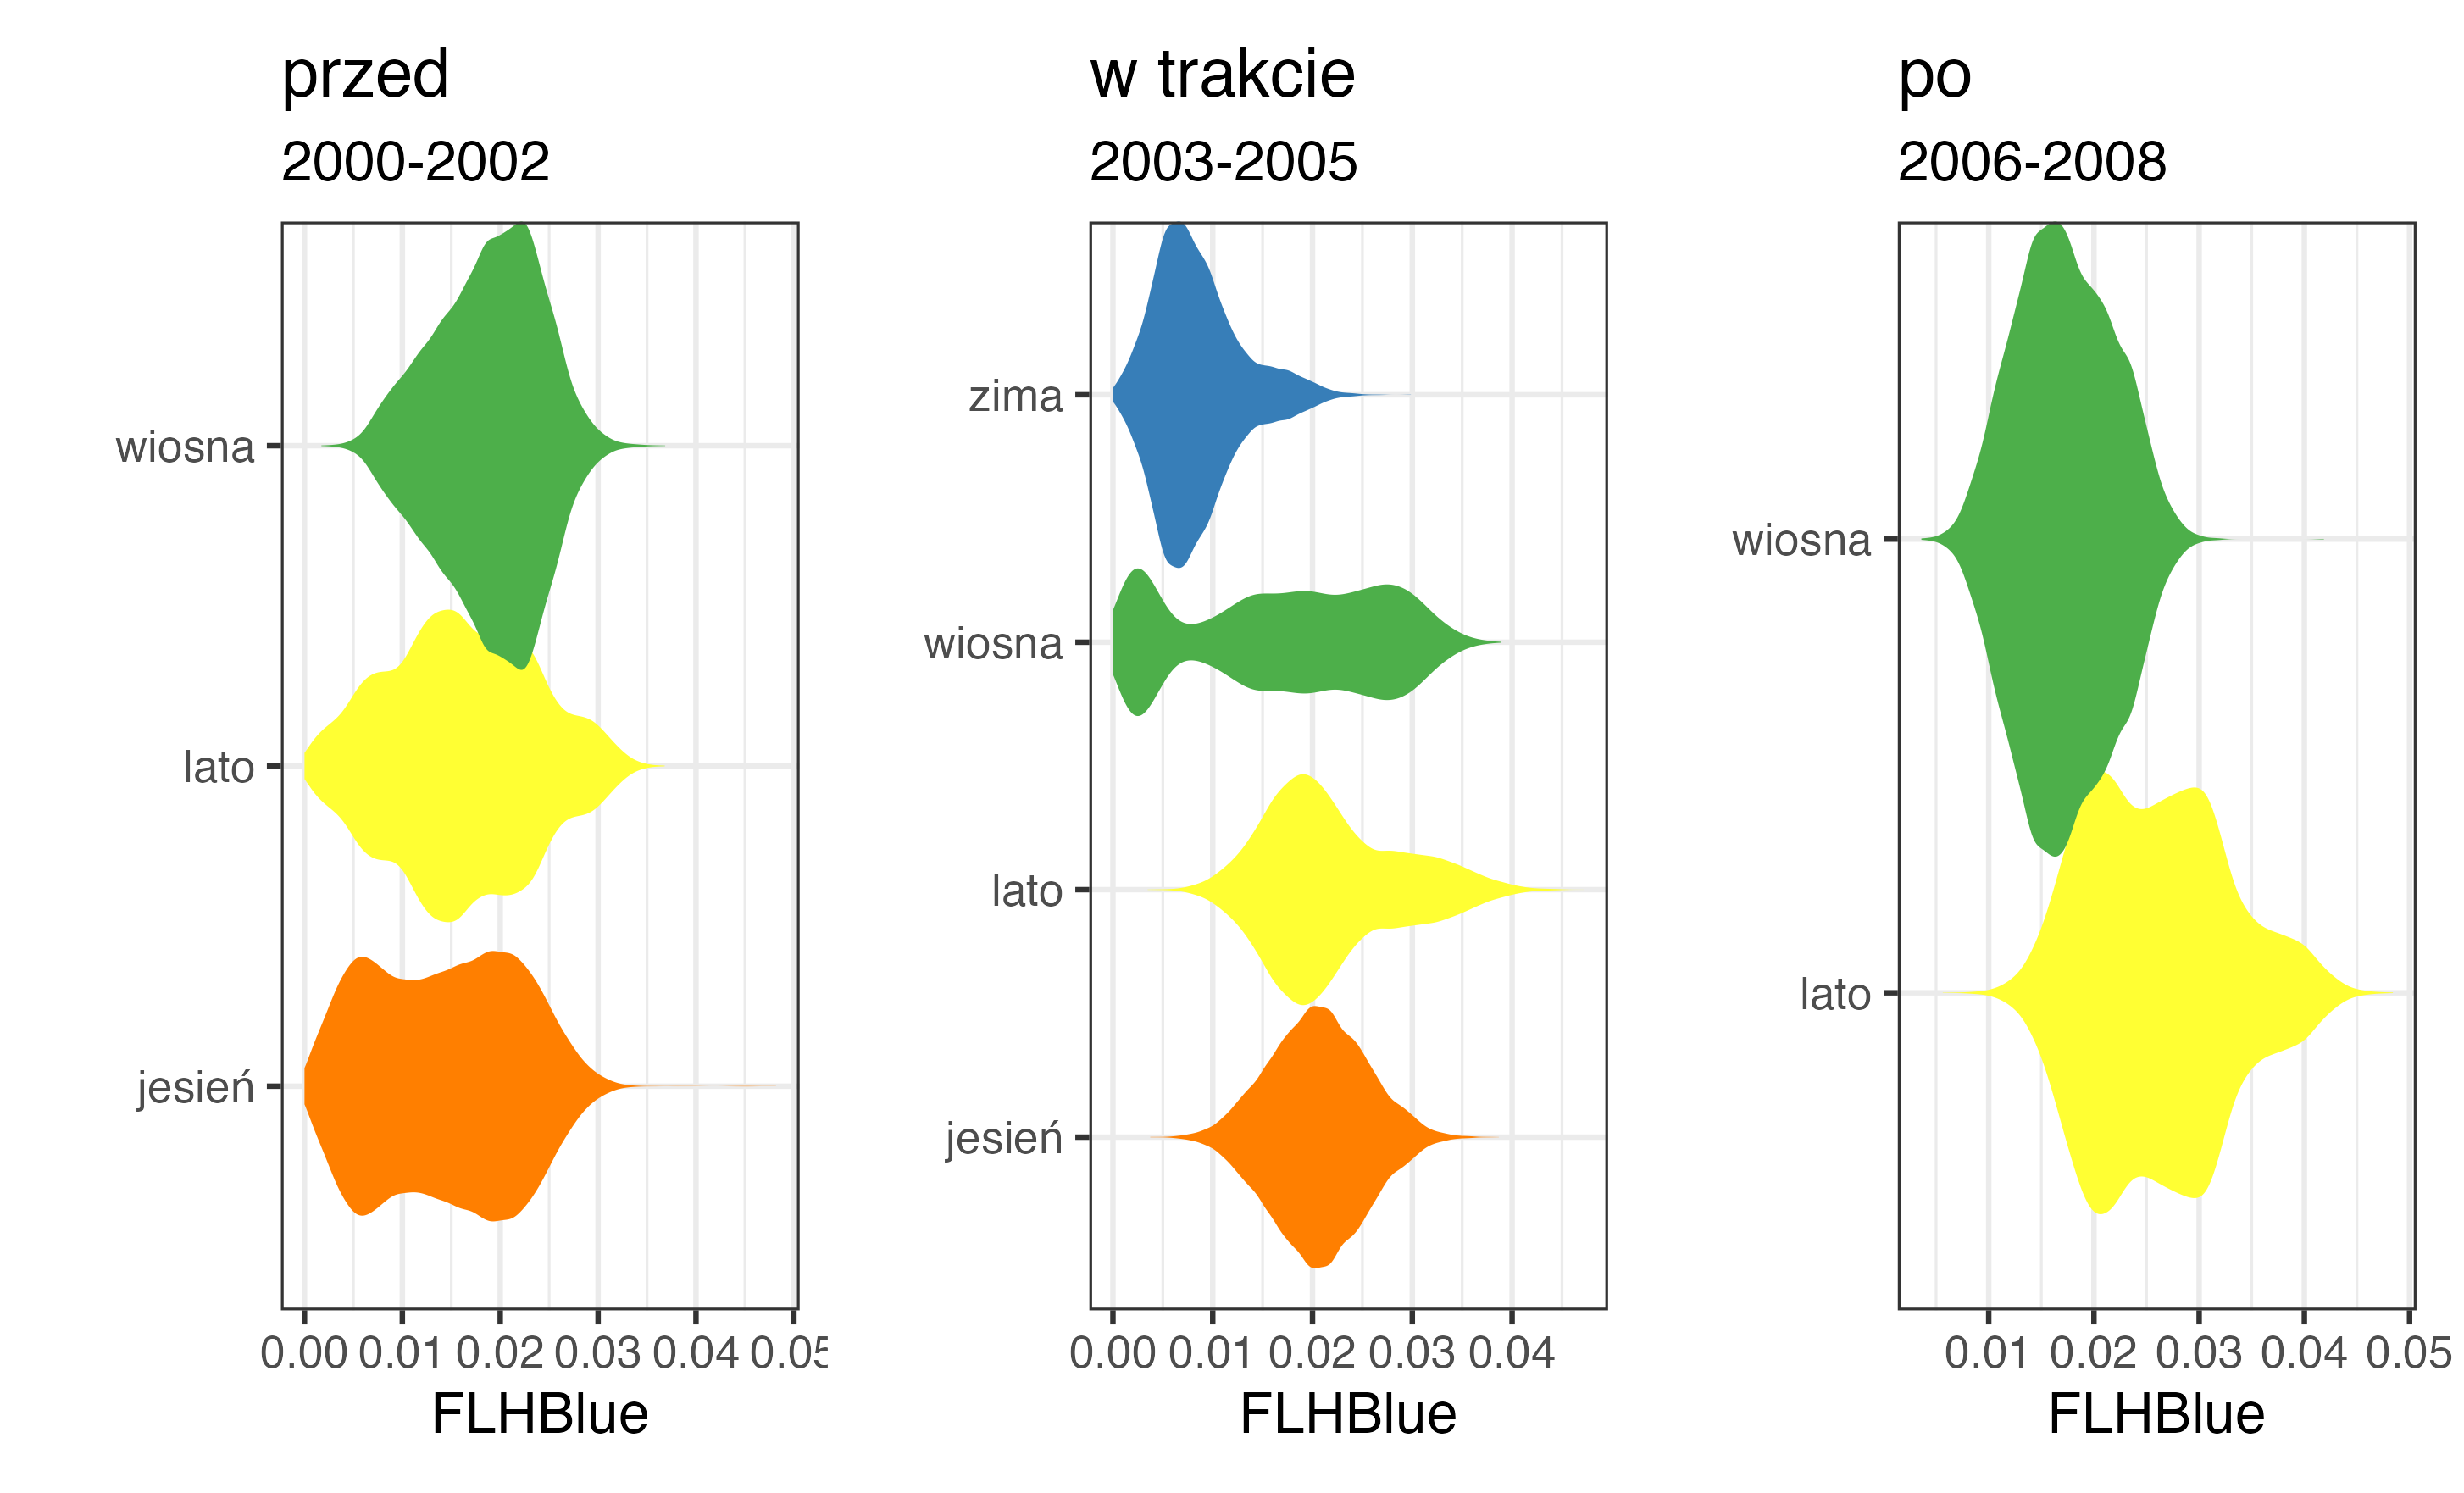
\includegraphics[width=6.25in,height=\textheight]{figures/china/flhblue_violin.png}

}

\caption{\label{fig-cn_flhblue_violin}Rozkład wartości stężenia
chlorofilu a dla Szanghaju według wskaźnika FLH Blue, z podziałem na
trzy etapy prac: przed rozpoczęciem, w trakcie i po zakończeniu prac,
oraz na cztery pory roku.}

\end{figure}

Rycina~\ref{fig-cn_flhblue_violin} przedstawia zmiany w rozkładach
średnich wartości stężenia chlorofilu a w Szanghaju. Etap tworzenia
nowych lądów wyróżnia się większym rozkładem wartości w porównaniu do
pozostałych okresów. Wartości w trakcie prowadzenia prac cechowały się
większą różnorodnością od wartości z pozostałych etapów, co jest
szczególnie widoczne dla wiosny. Rozkład średnich wartości wiosną
podczas prowadzenia prac znacząco różni się od rozkładu wartości wiosną
przed i po zakończeniu prac. Świadczy to o wpływie konstrukcji nowych
lądów na zwiększenie różnorodności stężenia chlorofilu a na obszarze
badań w Szanghaju.

\begin{figure}[t]

{\centering 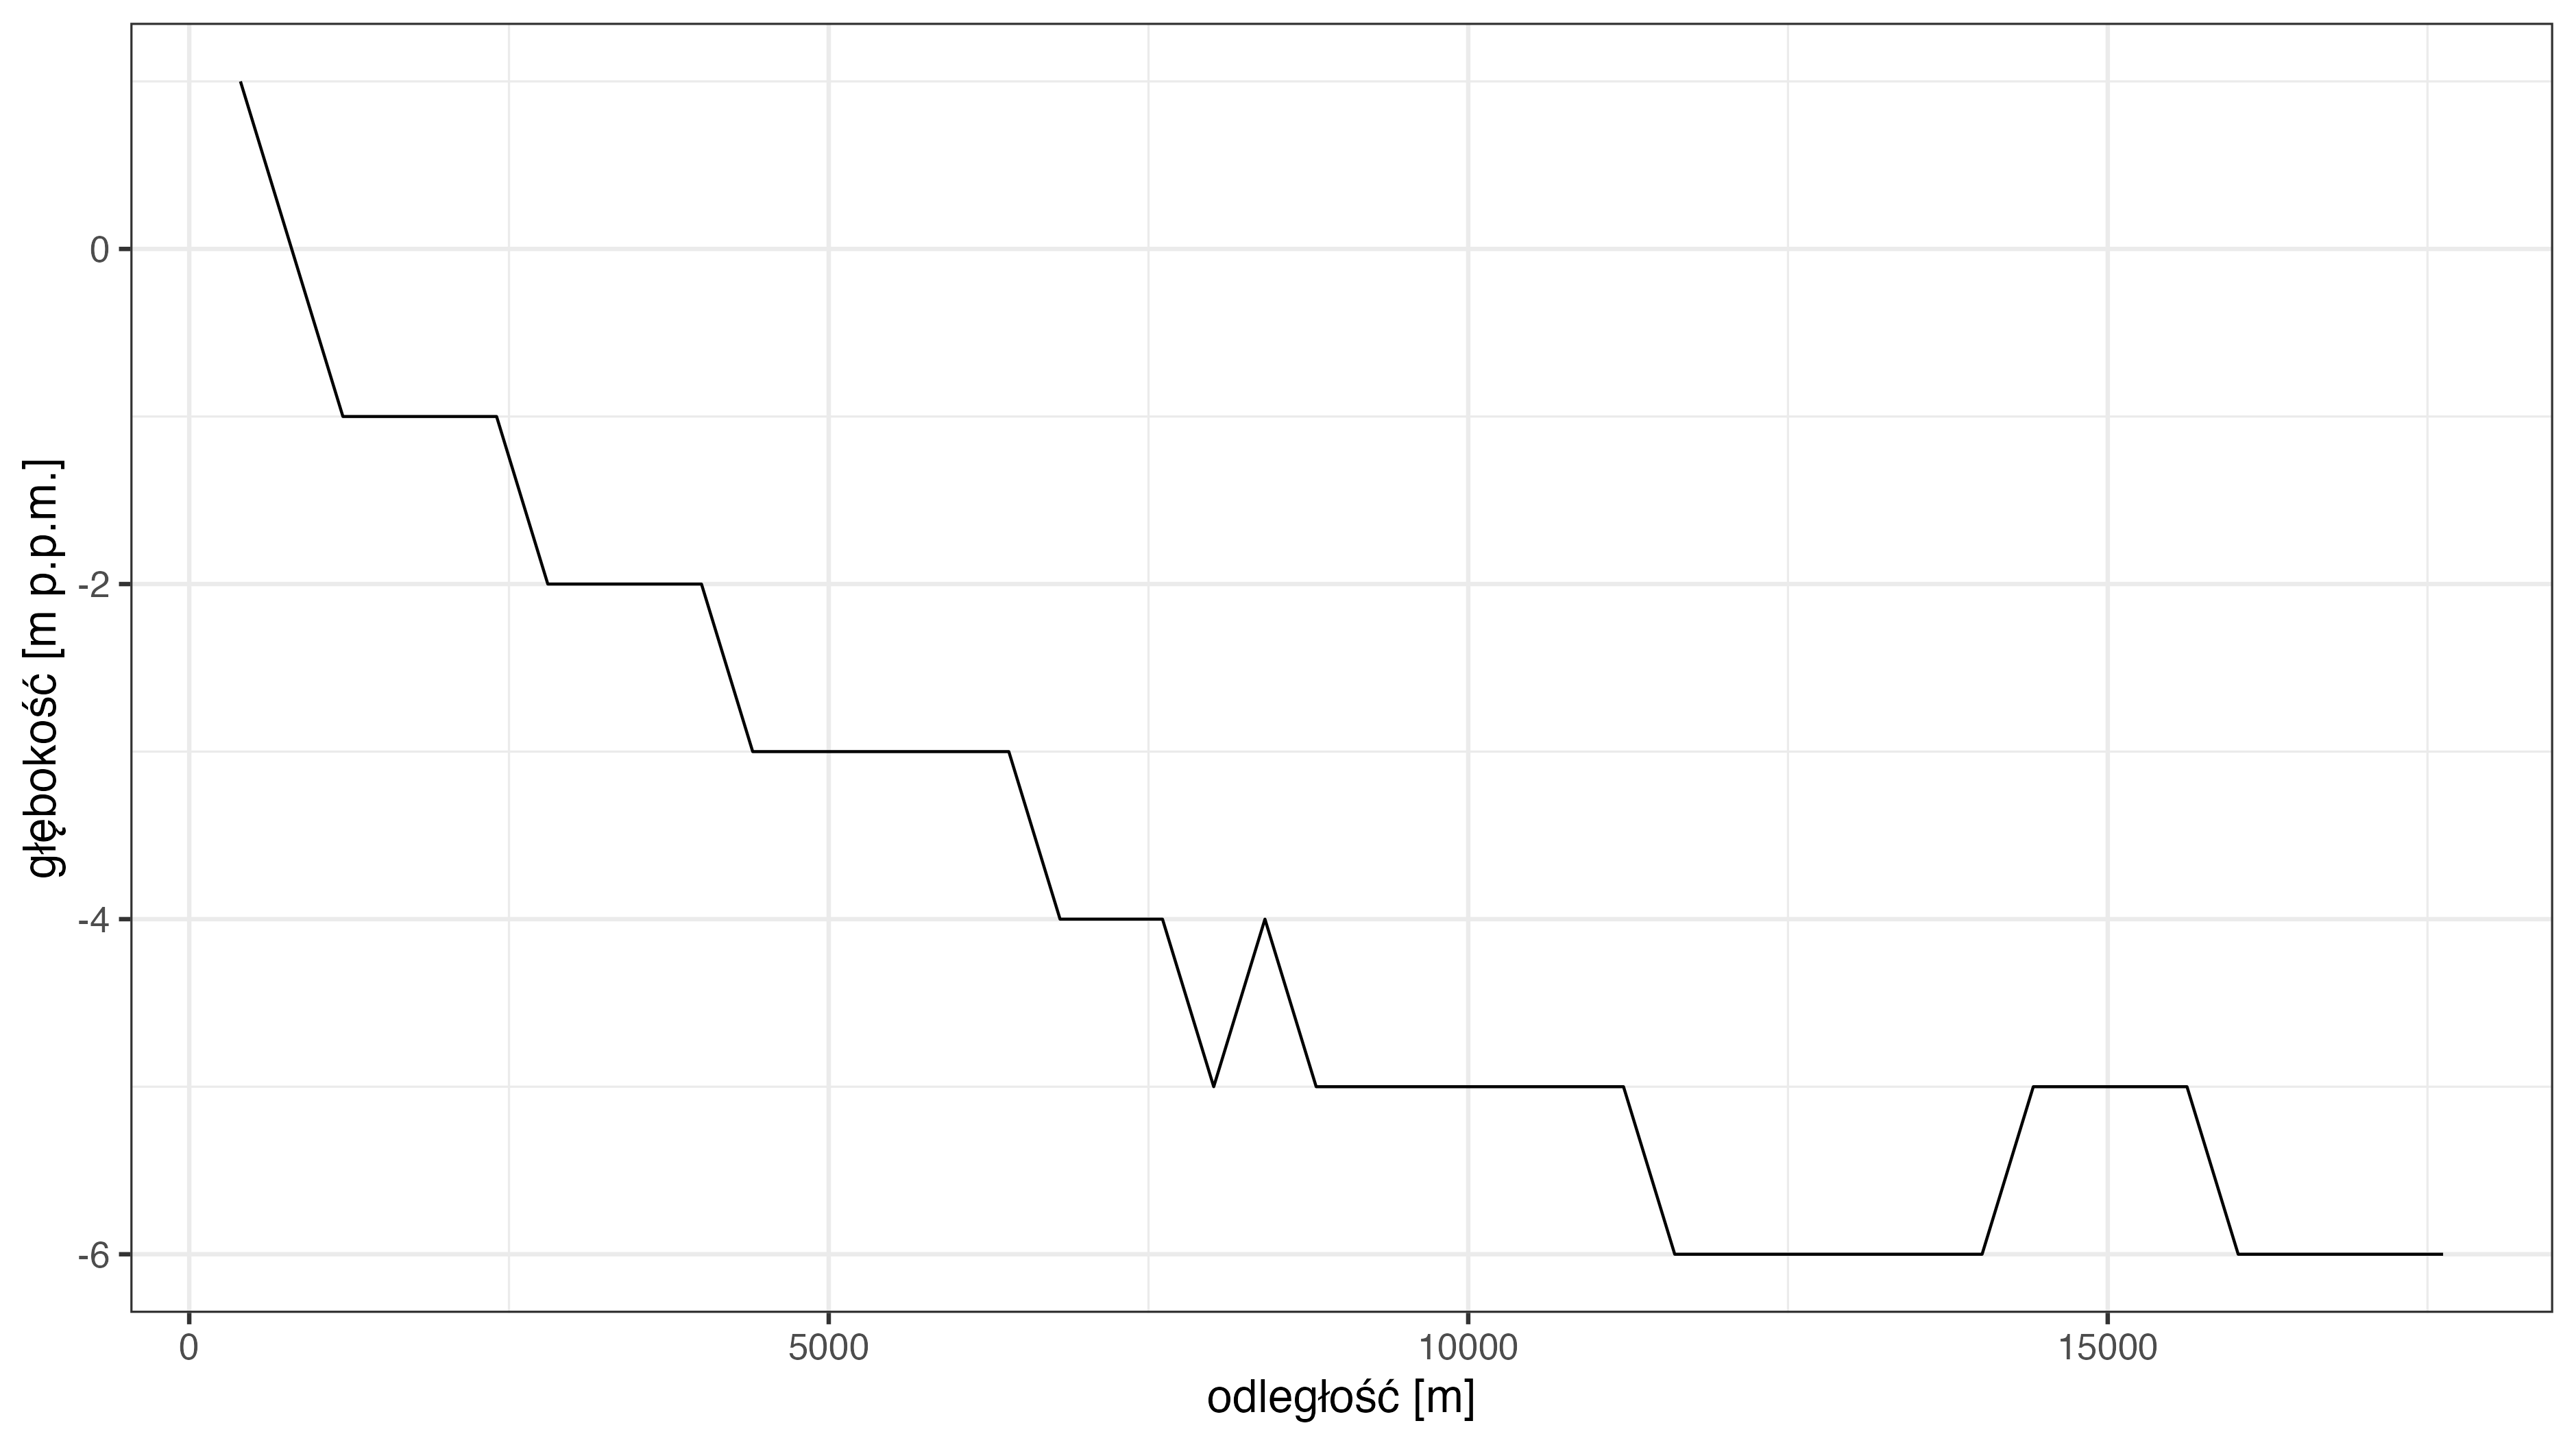
\includegraphics[width=3.64583in,height=\textheight]{figures/china/profile.png}

}

\caption{\label{fig-cn_profile}Zmiany głębokości zbiornika wodnego
wzdłuż profilu dla Szanghaju.}

\end{figure}

\begin{figure}[t]

{\centering 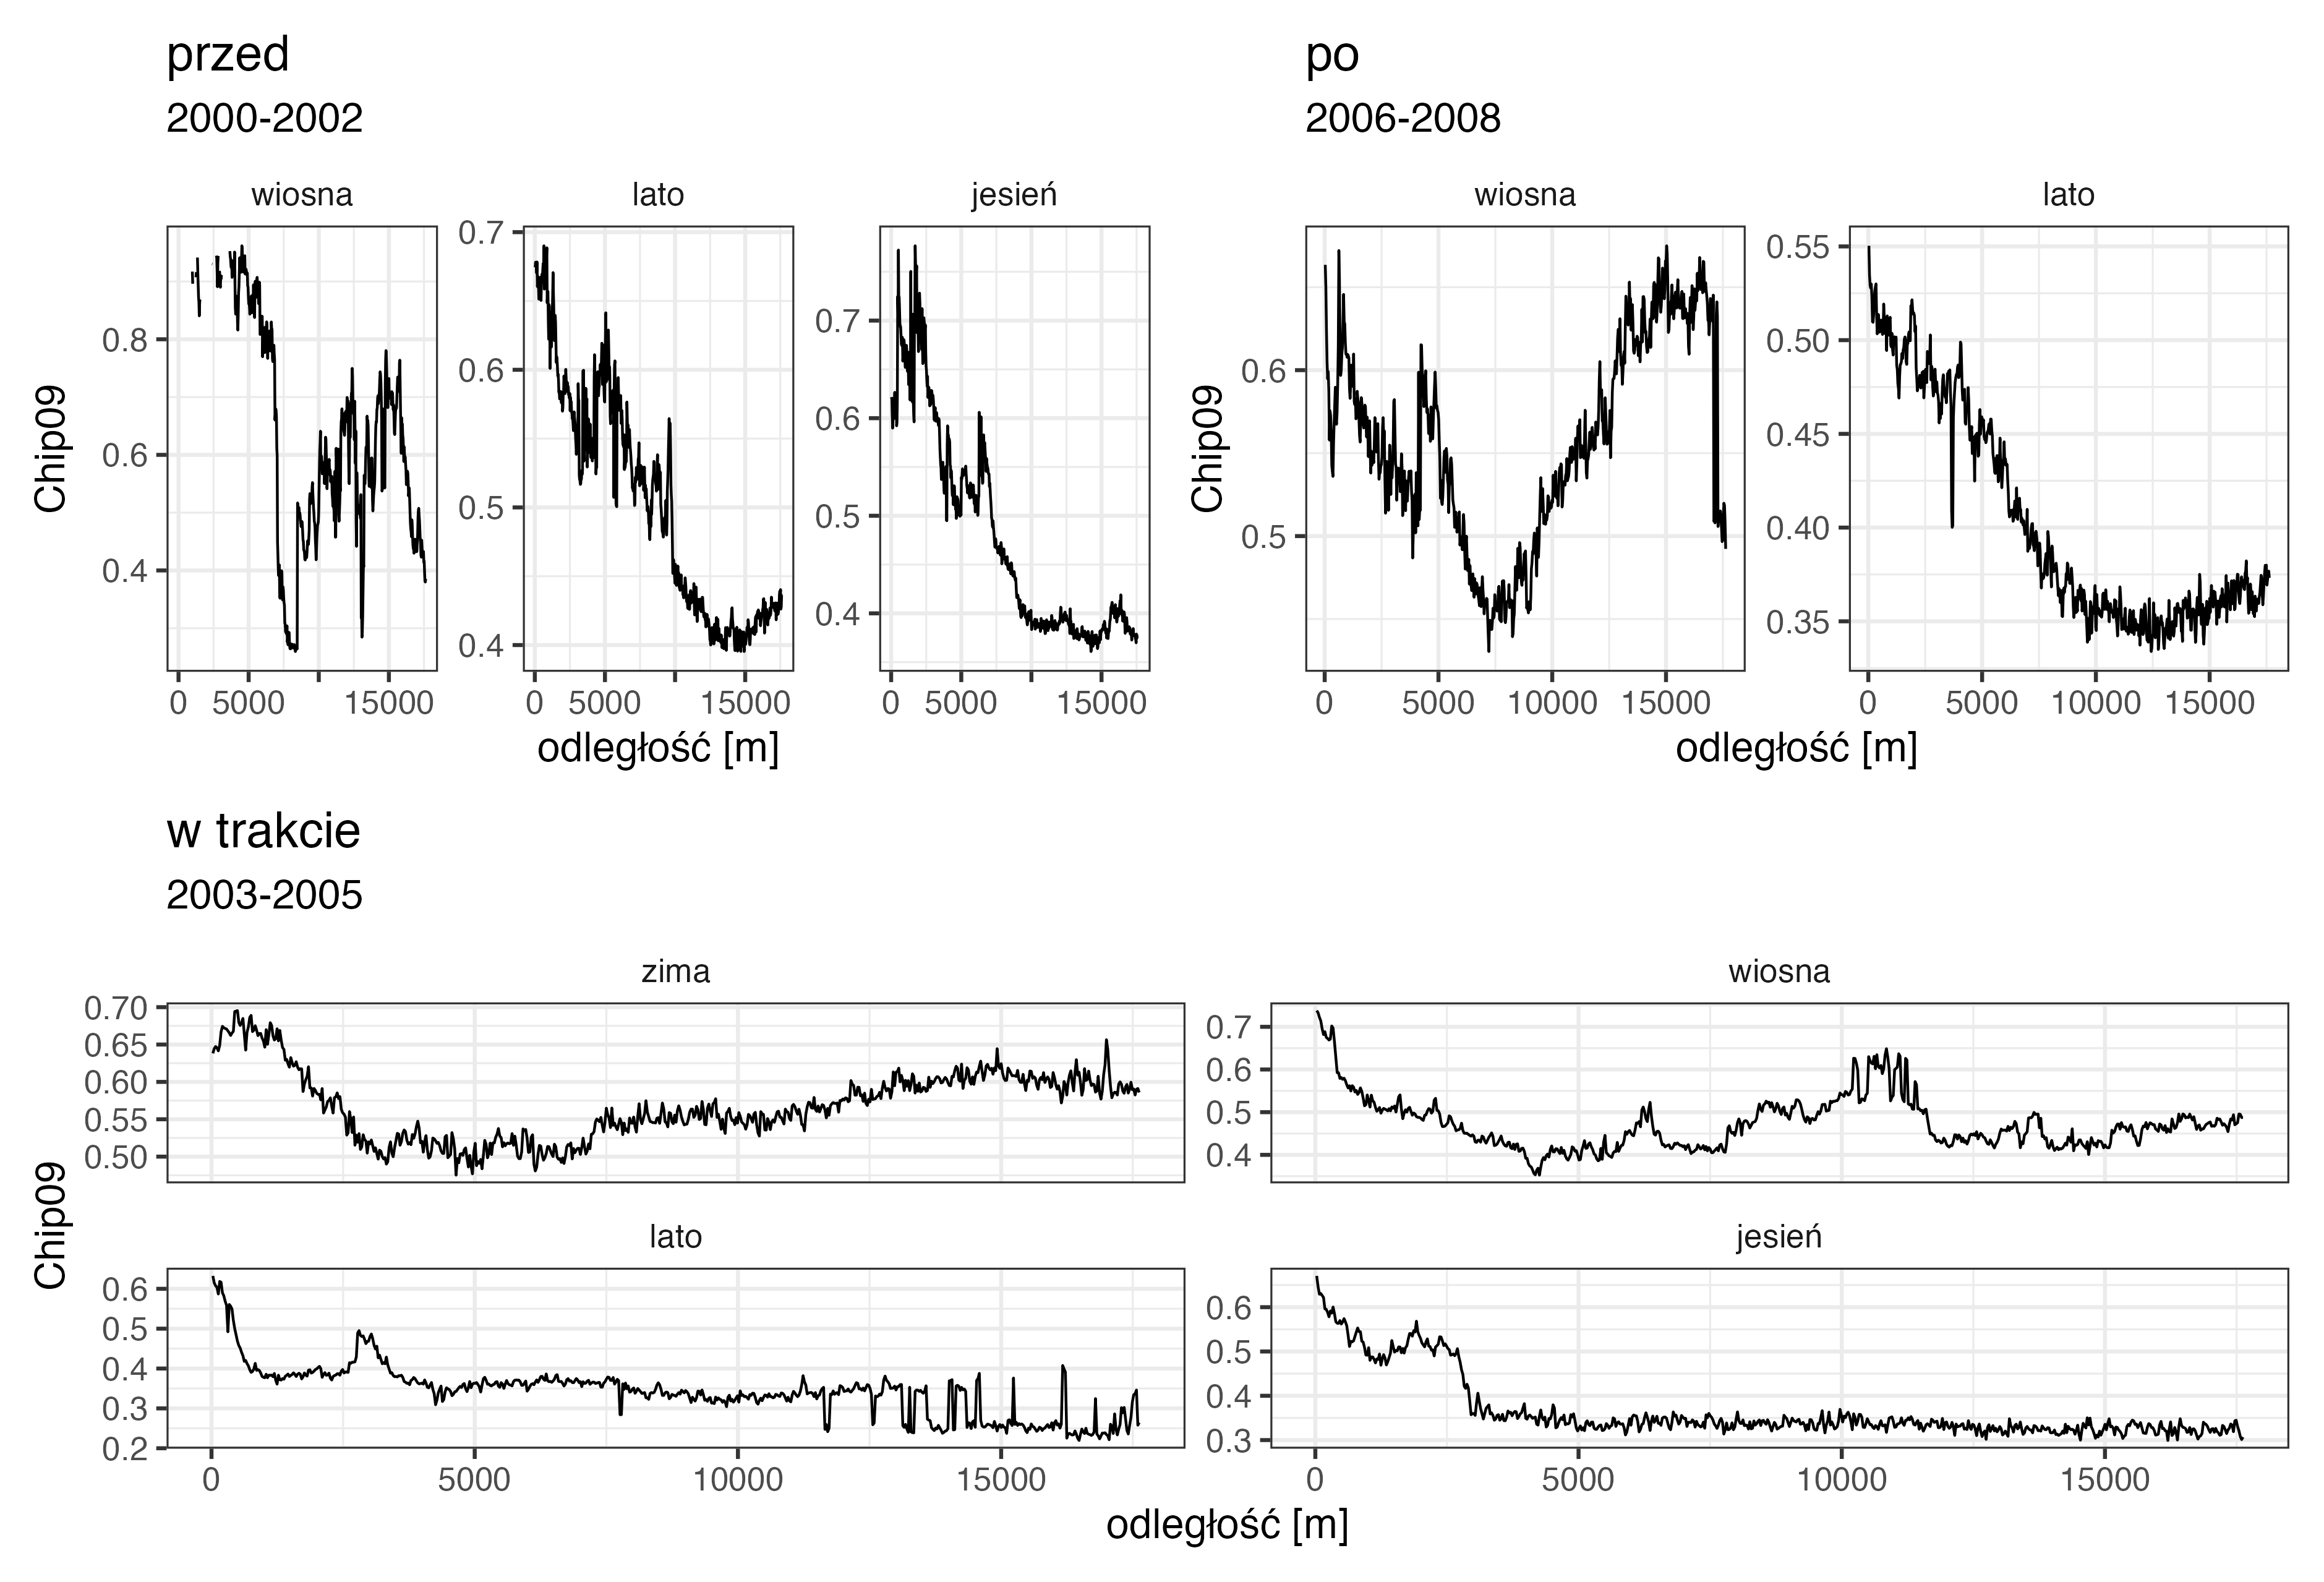
\includegraphics[width=6.77083in,height=\textheight]{figures/china/chip_profile.png}

}

\caption{\label{fig-cn_chip_profile}Zmiany wartości stężenia zawiesiny
wzdłuż profilu dla Szanghaju, przy wykorzysatniu wskaźnika Chip09.
Rycina składa się z trzech paneli: zmiany wartości dla obrazów przed
rozpoczęciem prac, w trakcie trwania prac i po zakończeniu prac. Każdy z
paneli podzielony jest na poszczególne pory roku. Czerwona linia jest
wygładzoną linią trendów.}

\end{figure}

Rycina~\ref{fig-cn_profile} pokazuje, że zbiornik wodny na obszarze
badań w Szanghaju osiąga maksymalną głębokość sześciu metrów.
Rycina~\ref{fig-cn_chip_profile} przedstawia, iż mimo małej różnicy
głębokości, zmiany stężenia zawiesiny w wodzie wykazują zależność ze
zmianą głębokości wzdłuż profilu. Zależność ta jest widoczna przed
rozpoczęciem prac tworzenia nowych lądów. Wraz z osiągnięciem odległości
2500 metrów wzdłuż profilu, stężenie zawiesiny zaczyna maleć.
Szczególnym przypadkiem jest wiosna, podczas której na odległości 8000
metrów stężenie zawiesiny zaczyna rosnąć. Trend ten jest również
widoczny podczas trwania prac i po ich zakończeniu. Zmiany stężenia
zawiesiny wiosną po zakończeniu prac są jednak większe niż przed ich
rozpoczęciem. Może to oznaczać potencjalny wpływ tworzenia nowych lądów
na powstawanie zaburzeń w rozkładzie przestrzennym stężeń zawiesiny,
zwłaszcza na obszarach położonych dalej od lądu.

\begin{figure}[t]

{\centering 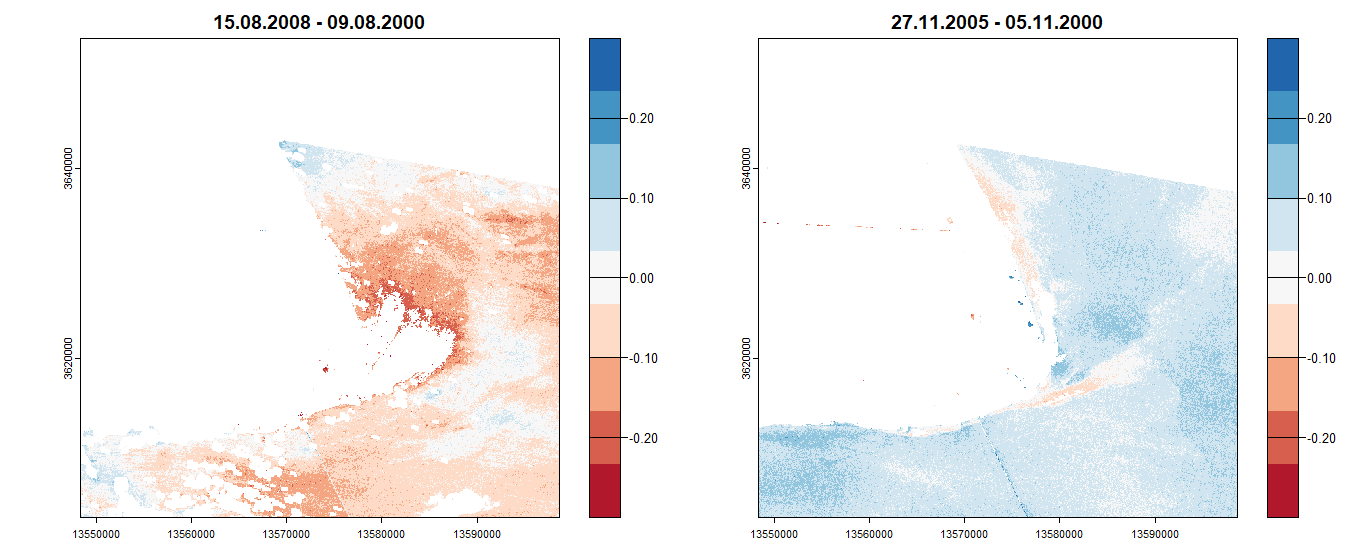
\includegraphics[width=6.25in,height=\textheight]{figures/china/sabi_diff.png}

}

\caption{\label{fig-cn_sabi_diff}Mapy różnic stężenia chlorofilu a dla
Szanghaju. Rycina po lewej przedstawia różnice między wskaźnikami,
obliczonymi w trakcie trwania i przed rozpoczęciem prac (maj 2005 i
2001). Rycina po prawej przedstawia różnice między wskaźnikami,
obliczonymi po zakończeniu prac i w trakcie ich trwania (sierpień 2008 i
2004).}

\end{figure}

Rycina~\ref{fig-cn_sabi_diff} przedstawia różnice w stężeniach
chlorofilu a na obszarze badań w Szanghaju. Lewa rycina pokazuje zmiany
w występowaniu chlorofilu a w trakcie trwania prac, zestawiając ich
wartości ze stanem przed rozpoczęciem prac. Wartości ujemne odpowiadają
spadkowi stężenia chlorofilu a wraz z rozpoczęciem prac tworzenia nowego
lądu. Odnotowane spadki stężenia chlorofilu a widoczne są na całym
obszarze badań, jednak największe zaobserwowano przy
północno--zachodniej części obszaru, na północ od strefy konstrukcji
nowego lądu. Prawa rycina pokazuje, w jaki sposób zakończenie prac
tworzenia nowych lądów wpłynęło na zmiany jakości wód. Wartości dodatnie
oznaczają wzrost stężenia chlorofilu a. Wartości ujemne odpowiadają
dalszemu spadkowi stężenia chlorofilu a. Najniższe wartości odnotowano
wzdłuż wybrzeża Szanghaju. Wskazuje to na długofalowe skutki konstrukcji
nowych lądów na jakość pobliskich wód. Wraz z oddalaniem się od
wybrzeża, stężenie chlorofilu a wzrasta. Wskazuje to na potencjalny
wpływ tworzenia nowych lądów na zmiany przestrzenne jakości wód.

Zmiany wartości wskaźnika FLH Blue, wskazujące na wzrost stężenia
chlorofilu a w Szanghaju po rozpoczęciu prac tworzenia nowych lądów,
wykazują istotność statystyczną. Spadek stężenia chlorofilu a odnotowano
jedynie w strefie przybrzeżnej. Zmiany stężenia zawiesiny wskazują na
pogorszenie jakości wód, ponieważ po rozpoczęciu tworzenia nowych lądów
mętność wody stale wzrastała. Odnotowano także zaburzenia w rozkładzie
przestrzennym stężeń zawiesiny. Zmiany stężenia zawiesiny w wodzie dla
obszaru badań w Szanghaju były jednak najmniejszymi odnotowanymi
zmianami, spośród wszystkich obszarów badań. Dodatkowo, mętność wody
przed rozpoczęciem prac na obszarze badań w Szanghaju była najwyższa
spośród wszystkich obszarów. Wskazuje to na potencjalnie niski wpływ
tworzenia nowych lądów na zmiany parametru jakości wód, jakim jest
mętność wody.

\bookmarksetup{startatroot}

\hypertarget{podsumowanie}{%
\chapter{Podsumowanie}\label{podsumowanie}}

Wyniki przeprowadzonych badań wskazały na wpływ tworzenia nowych lądów
na stan jakości wód na każdym z obszarów. Konstrukcja nowych lądów
wpłynęła na spadek stężenia chlorofilu a w Dubaju, Limon i Singapurze.
Największą różnicę zaobserwowano w Limon. W Dubaju i Singapurze,
stężenie chlorofilu było jeszcze niższe po zakończeniu prac. Może to
wynikać ze sposobu wykorzystania nowych lądów na obydwu obszarach badań.
Praca \textcite{zhang2017assessment} wykazała podobną zależność, gdzie
największy udział w degradacji jakości wód miały zakłady przemysłowe,
powstałe na nowych terenach lądowych. W Singapurze, nowy ląd posłużył
rozbudowie lotniska i bazy marynarki wojennej kraju. Nowe tereny w
Dubaju zostały wykorzystane natomiast pod rozbudowę infrastruktury
turystycznej, tworząc fundamenty pod nowe hotele i atrakcje turystyczne.

W Lagos i Szanghaju, wraz z rozpoczęciem tworzenia nowych lądów,
zanotowano wzrost stężenia chlorofilu a. Wzrost ten utrzymał się po
zakończeniu prac. Obydwa obszary łączy sposób wykorzystania nowych
lądów, które zostały przeznaczone pod strefy mieszkalne. Praca
\textcite{zhang2017assessment} proponowała rozwiązanie problemu, gdzie
uzdatnianie wody miało posłużyć się poprawie jakości wód po stworzeniu
nowych lądów. Wskazuje to na pośredni wpływ tworzenia nowych lądów na
jakość wód, wynikające z wprowadzenia regulacji i programów ochrony w
celu poprawy jakości wód.

Wpływ tworzenia nowego lądu na wzrost stężenia zawiesiny odnotowano w
Dubaju, Limon i Szanghaju. Dla tych samych obszarów, stężenie zawiesiny
po zakończeniu prac konstrukcyjnych zmalało. Wskazuje to tymczasowy
wzrost mętności wody, spowodowany trwaniem prac nad tworzeniem nowych
lądów. Oznacza to, że w tych trzech obszarach, tworzenie nowych lądów ma
negatywny wpływ na jakość wód, zwiększając ich mętność. Spowodowane to
może być długim okresem trwania prac. W Dubaju, Limon i Szanghaju,
tworzenie nowego lądu trwało krócej, w porównaniu do długości prac w
Lagos i Singapurze. Wykorzystane techniki, które przysłużyły się do
przyspieszenia prac, mogły jednocześnie przyczynić się do większej
degradacji jakości wody.

Na obszarach badań w Lagos i Singapurze odnotowano spadek mętności wody
po rozpoczęciu prac nad konstrukcją nowych terenów. W obydwu miejscach,
stężenie zawiesiny dalej zmniejszało się po zakończeniu prac. Może to
świadczyć o małym wpływie tworzenia nowych lądów na zmiany mętności wody
i stanu jakości wód dla tych obszarów. Zmiany mętności w czasie na tych
obszarach badań świadczą o występowaniu innego czynnika,
przyczyniającego się do spadku stężenia zawiesiny w wodzie. Do
potwierdzenia tej tezy konieczna jest dodatkowa analiza, obejmująca
szerszy zakres czasowy niż uwzględniony w tej pracy.

Wyniki tej pracy wskazują na zgodność z wynikami prac, przytoczonymi w
przeglądzie literatury. Praca \textcite{hao2021effects} wskazuje na
największe zmiany w parametrach jakości wód w okresie tworzenia nowych
lądów. Stężenie metali ciężkich tuż po zakończeniu prac było większe,
niż przed rozpoczęciem budowy. Taką samą zależność odnotowano w tej
pracy. Wraz z rozpoczęciem konstrukcji nowych lądów, odnotowane zostały
zmiany w wartościach parametrów jakości wód. Praca
\textcite{wang2023observations} również dochodzi do podobnych wniosków.
Konstrukcja nowych lądów pod budowę lotniska przyczyniła się do
zwiększenia mętności wody i zwiększenia stężenia nieorganicznego azotu w
wodzie.

Użycie czterech wskaźników, opisujących dwa parametry, dało wgląd na
szeroki zakres stanu jakości wód. Spośród wszystkich wykorzystanych
wskaźników, FLH Blue badający stężenie chlorofilu a przysłużył się
dwukrotnie do wykazania istotności statystycznej między średnimi
wartościami stężenia chlorofilu a a poszczególnymi etapami prac.
Wskazuje to na potencjał tego wskaźnika w dalszych badaniach jakości
wód. W badaniach wykryto, że wzrost liczby obserwacji koreluje ze
wzrostem istotności statystycznej. Zwiększenie zakresu czasowego, albo
zastosowanie innej metody wyboru obrazów satelitarnych może w przyszłych
badaniach zwiększyć liczbę obserwacji i przysłużyć się do zwiększenia
jakości wyników.

Dodanie do zakresu czasowego badań dodatkowych lat przed rozpoczęciem i
po zakończeniu prac dostarczyło duży zasób informacji. Porównanie
wartości parametrów jakości wód z fazy tworzenia lądów z wartościami
przed rozpoczęciem prac pozwoliło zaobserwować bezpośrednie zmiany,
wywołane pracami. Analiza stężeń chlorofilu a i zawiesiny po zakończeniu
prac umożliwiło wykrycie potencjalnych długofalowych skutków tworzenia
lądu na zmiany jakości wód. W kolejnych badaniach, metoda ta może zostać
usprawniona. Etapy przed i po zakończeniu prac obejmowały osobno od
dwóch do trzech lat. Okres trwania prac nad tworzeniem lądów natomiast
potrafił zajmować od dwóch do nawet dziesięciu lat. Prowadziło to do
powstania niezbalansowanych grup, w których większość obserwacji
należała do etapu trwania prac. Rozszerzenie zakresu czasowego dla
etapów przed rozpoczęciem i po zakończeniu tworzenia nowego lądu
pozwoliłoby również wykryć długookresowe zmiany w jakościach wód i
odseparować je od zmian wywołanych przez procesy tworzenia lądów.
Dostarczyłoby to jeszcze dokładniejsze wyniki wpływu tworzenia nowych
lądów na stan wód.

Wybrane obszary badań dostarczyły dużą ilość informacji i przysłużyły
się do odkrycia potencjalnych zależności. Dużym walorem była ich
różnorodność w wykorzystaniu nowego lądu. Pozwoliło to odkryć
zależności, występujące między osobnymi obszarami o podobnych rodzajach
zastosowań nowego terenu. Wybór obszarów z różnych części świata i
zakresów czasowych również okazał się przydatny do zaobserwowania różnic
we wpływach tworzenia nowych lądów na stan jakości wód.

W wyniku ograniczeń, w pracy zrezygnowano z kilku ulepszeń, mogących
przyczynić się do pozyskania lepszej jakości wyników. Jeden z
potencjalnych usprawnień w ramach pracy dotyczyłby oceny jakości wody. W
ramach pracy, zmiany jakości wód były oceniane poprzez porównywanie
zmian parametrów w czasie, oraz porównując je między obszarami badań.
Wszystkie obszary badań obejmowały tereny, na których przeprowadzane
były konstrukcje nowych lądów. W celu zwiększenia dokładności wyników,
ocenę zmian jakości wód powinno się także przeprowadzić na obszarach, na
których nie miały miejsca prace tworzenia nowych lądów. Pozwoliłoby to
na sprawdzenie, czy zmiany jakości wód faktycznie wynikały z tworzenia
nowych lądów, czy były wynikiem regionalnych zmian jakości wód.
Dodatkowe obszary badań powinny być jak najbardziej zbliżone do
wybranych obszarów. Podobieństwo polegałoby na podobnym ukształtowaniu
dna zbiornika wodnego i terenu na wybrzeżu, podobnym wykorzystaniu
terenu wybrzeżnego, czy podobnych parametrach pogody. Wprowadzenie
takiego ulepszenia wymagałoby zaproponowania metody, służącej do
odnajdywania bliźniaczych terenów dla wybranego obszaru badań. Metoda
ta, po zapoznaniu się z własnościami obszaru badań na którym utworzono
nowy ląd, powinna odnaleźć inny obszar o podobnych parametrach, na
którym nie wykonywano prac tworzenia nowych lądów. Opracowanie tej
metody okazało się zbyt czasochłonne i nie zostało uwzględnione w tej
pracy.

Oprócz dodatkowych obszarów badań, wykorzystanie dodatkowych parametrów
jakości wód również mogłoby skutkować wykonaniem dokładniejszych badań.
W pracy wykorzystano obrazy satelitarne oraz dane o batymetrii.
Pozwoliło to na ocenę zmian fizycznych parametrów wodnych (chlorofil a,
mętność wody), możliwych do obserwacji z poziomu obrazów satelitarnych.
Dodatkowe źródła danych pozwoliłyby na badanie zmian biologicznych i
chemicznych parametrów jakości wód w trakcie tworzenia nowych lądów. Do
takich parametrów należą między innymi temperatura wody, zasolenie,
zasadowość, stężenie nieorganicznego azotu czy metali ciężkich.

Inne ulepszenie dotyczyłoby zmiany metody pozyskiwania zdjęć
satelitarnych. Metoda wykorzystana w tej pracy pozwoliła na pozyskanie
dużego zbioru obrazów. Jednak większość z tych zdjęć nie była przydatna
do wykorzystania w dalszej analizie. Wynikało to ze sposobu maskowania
danych, niebędących zbiornikami wodnymi. Wykorzystanie kanału QA
pozwoliło na wybór komórek rastrów przypisanych do klasy zbiorników
wodnych bez pokrycia chmurami. Skutkowało to powstawaniem wielu luk i
przerw w obrazach satelitarnych, co ograniczało możliwości
przeprowadzania analiz przestrzennych. Możliwym rozwiązaniem tego
problemu jest zaproponowanie lepszej metody maskowania obszarów
niebędących zbiornikami wodnymi. Metoda ta mogłaby być rozwinięciem
stosowania kanału QA i polegać na wyborze dodatkowych klas. Podejście to
nie rozwiąże jednak problemu z występowaniem zachmurzeń, które wyklucza
z analizy obszary będące zakryte chmurami. Alternatywnym rozwiązaniem
jest stosowanie kompozytów. Zamiast pracować na zdjęciach satelitarnych
z pojedynczych dni, można utworzyć z kilku zdjęć jeden obraz, będący
całkowicie wypełniony informacjami. Potencjalne podejście polegałoby na
grupowaniu zdjęć według miesięcy. Dla każdego miesiąca wyliczany byłby
jeden obraz kompozytowy. Wartości komórek obrazu kompozytowego mógłby
być medianą wszystkich dostępnych wartości komórek z pojedynczych zdjęć.
Takie rozwiązanie umożliwiłoby pozyskanie obrazu w całości wypełnionego
danymi. Wadą tej metody jest fakt, że obraz kompozytowy nie jest
odzwierciedleniem obszaru w konkretnym momencie, a mozaiką informacji,
złączoną z wielu różnych obrazów. Może to spowodować powstanie wzorców
przestrzennych, nie mających odzwierciedlenia w rzeczywistości i
prowadzących do nieprawdziwych wniosków. Między innymi z tego powodu w
pracy zdecydowano się korzystać z pojedynczych obrazów satelitarnych.

\bookmarksetup{startatroot}

\hypertarget{bibliografia}{%
\chapter*{Bibliografia}\label{bibliografia}}
\addcontentsline{toc}{chapter}{Bibliografia}

\markboth{Bibliografia}{Bibliografia}

\printbibliography[heading=none]

%\printbibliography[heading=bibintoc, title=Bibliografia]

\end{document}
